% Options for packages loaded elsewhere
% Options for packages loaded elsewhere
\PassOptionsToPackage{unicode}{hyperref}
\PassOptionsToPackage{hyphens}{url}
%
\documentclass[
  12pt,
  letterpaper,
]{scrbook}
\usepackage{xcolor}
\usepackage{amsmath,amssymb}
\setcounter{secnumdepth}{5}
\usepackage{iftex}
\ifPDFTeX
  \usepackage[T1]{fontenc}
  \usepackage[utf8]{inputenc}
  \usepackage{textcomp} % provide euro and other symbols
\else % if luatex or xetex
  \usepackage{unicode-math} % this also loads fontspec
  \defaultfontfeatures{Scale=MatchLowercase}
  \defaultfontfeatures[\rmfamily]{Ligatures=TeX,Scale=1}
\fi
\usepackage{lmodern}
\ifPDFTeX\else
  % xetex/luatex font selection
\fi
% Use upquote if available, for straight quotes in verbatim environments
\IfFileExists{upquote.sty}{\usepackage{upquote}}{}
\IfFileExists{microtype.sty}{% use microtype if available
  \usepackage[]{microtype}
  \UseMicrotypeSet[protrusion]{basicmath} % disable protrusion for tt fonts
}{}
\makeatletter
\@ifundefined{KOMAClassName}{% if non-KOMA class
  \IfFileExists{parskip.sty}{%
    \usepackage{parskip}
  }{% else
    \setlength{\parindent}{0pt}
    \setlength{\parskip}{6pt plus 2pt minus 1pt}}
}{% if KOMA class
  \KOMAoptions{parskip=half}}
\makeatother
% Make \paragraph and \subparagraph free-standing
\makeatletter
\ifx\paragraph\undefined\else
  \let\oldparagraph\paragraph
  \renewcommand{\paragraph}{
    \@ifstar
      \xxxParagraphStar
      \xxxParagraphNoStar
  }
  \newcommand{\xxxParagraphStar}[1]{\oldparagraph*{#1}\mbox{}}
  \newcommand{\xxxParagraphNoStar}[1]{\oldparagraph{#1}\mbox{}}
\fi
\ifx\subparagraph\undefined\else
  \let\oldsubparagraph\subparagraph
  \renewcommand{\subparagraph}{
    \@ifstar
      \xxxSubParagraphStar
      \xxxSubParagraphNoStar
  }
  \newcommand{\xxxSubParagraphStar}[1]{\oldsubparagraph*{#1}\mbox{}}
  \newcommand{\xxxSubParagraphNoStar}[1]{\oldsubparagraph{#1}\mbox{}}
\fi
\makeatother

\usepackage{color}
\usepackage{fancyvrb}
\newcommand{\VerbBar}{|}
\newcommand{\VERB}{\Verb[commandchars=\\\{\}]}
\DefineVerbatimEnvironment{Highlighting}{Verbatim}{commandchars=\\\{\}}
% Add ',fontsize=\small' for more characters per line
\usepackage{framed}
\definecolor{shadecolor}{RGB}{241,243,245}
\newenvironment{Shaded}{\begin{snugshade}}{\end{snugshade}}
\newcommand{\AlertTok}[1]{\textcolor[rgb]{0.68,0.00,0.00}{#1}}
\newcommand{\AnnotationTok}[1]{\textcolor[rgb]{0.37,0.37,0.37}{#1}}
\newcommand{\AttributeTok}[1]{\textcolor[rgb]{0.40,0.45,0.13}{#1}}
\newcommand{\BaseNTok}[1]{\textcolor[rgb]{0.68,0.00,0.00}{#1}}
\newcommand{\BuiltInTok}[1]{\textcolor[rgb]{0.00,0.23,0.31}{#1}}
\newcommand{\CharTok}[1]{\textcolor[rgb]{0.13,0.47,0.30}{#1}}
\newcommand{\CommentTok}[1]{\textcolor[rgb]{0.37,0.37,0.37}{#1}}
\newcommand{\CommentVarTok}[1]{\textcolor[rgb]{0.37,0.37,0.37}{\textit{#1}}}
\newcommand{\ConstantTok}[1]{\textcolor[rgb]{0.56,0.35,0.01}{#1}}
\newcommand{\ControlFlowTok}[1]{\textcolor[rgb]{0.00,0.23,0.31}{\textbf{#1}}}
\newcommand{\DataTypeTok}[1]{\textcolor[rgb]{0.68,0.00,0.00}{#1}}
\newcommand{\DecValTok}[1]{\textcolor[rgb]{0.68,0.00,0.00}{#1}}
\newcommand{\DocumentationTok}[1]{\textcolor[rgb]{0.37,0.37,0.37}{\textit{#1}}}
\newcommand{\ErrorTok}[1]{\textcolor[rgb]{0.68,0.00,0.00}{#1}}
\newcommand{\ExtensionTok}[1]{\textcolor[rgb]{0.00,0.23,0.31}{#1}}
\newcommand{\FloatTok}[1]{\textcolor[rgb]{0.68,0.00,0.00}{#1}}
\newcommand{\FunctionTok}[1]{\textcolor[rgb]{0.28,0.35,0.67}{#1}}
\newcommand{\ImportTok}[1]{\textcolor[rgb]{0.00,0.46,0.62}{#1}}
\newcommand{\InformationTok}[1]{\textcolor[rgb]{0.37,0.37,0.37}{#1}}
\newcommand{\KeywordTok}[1]{\textcolor[rgb]{0.00,0.23,0.31}{\textbf{#1}}}
\newcommand{\NormalTok}[1]{\textcolor[rgb]{0.00,0.23,0.31}{#1}}
\newcommand{\OperatorTok}[1]{\textcolor[rgb]{0.37,0.37,0.37}{#1}}
\newcommand{\OtherTok}[1]{\textcolor[rgb]{0.00,0.23,0.31}{#1}}
\newcommand{\PreprocessorTok}[1]{\textcolor[rgb]{0.68,0.00,0.00}{#1}}
\newcommand{\RegionMarkerTok}[1]{\textcolor[rgb]{0.00,0.23,0.31}{#1}}
\newcommand{\SpecialCharTok}[1]{\textcolor[rgb]{0.37,0.37,0.37}{#1}}
\newcommand{\SpecialStringTok}[1]{\textcolor[rgb]{0.13,0.47,0.30}{#1}}
\newcommand{\StringTok}[1]{\textcolor[rgb]{0.13,0.47,0.30}{#1}}
\newcommand{\VariableTok}[1]{\textcolor[rgb]{0.07,0.07,0.07}{#1}}
\newcommand{\VerbatimStringTok}[1]{\textcolor[rgb]{0.13,0.47,0.30}{#1}}
\newcommand{\WarningTok}[1]{\textcolor[rgb]{0.37,0.37,0.37}{\textit{#1}}}

\usepackage{longtable,booktabs,array}
\usepackage{calc} % for calculating minipage widths
% Correct order of tables after \paragraph or \subparagraph
\usepackage{etoolbox}
\makeatletter
\patchcmd\longtable{\par}{\if@noskipsec\mbox{}\fi\par}{}{}
\makeatother
% Allow footnotes in longtable head/foot
\IfFileExists{footnotehyper.sty}{\usepackage{footnotehyper}}{\usepackage{footnote}}
\makesavenoteenv{longtable}
\usepackage{graphicx}
\makeatletter
\newsavebox\pandoc@box
\newcommand*\pandocbounded[1]{% scales image to fit in text height/width
  \sbox\pandoc@box{#1}%
  \Gscale@div\@tempa{\textheight}{\dimexpr\ht\pandoc@box+\dp\pandoc@box\relax}%
  \Gscale@div\@tempb{\linewidth}{\wd\pandoc@box}%
  \ifdim\@tempb\p@<\@tempa\p@\let\@tempa\@tempb\fi% select the smaller of both
  \ifdim\@tempa\p@<\p@\scalebox{\@tempa}{\usebox\pandoc@box}%
  \else\usebox{\pandoc@box}%
  \fi%
}
% Set default figure placement to htbp
\def\fps@figure{htbp}
\makeatother





\setlength{\emergencystretch}{3em} % prevent overfull lines

\providecommand{\tightlist}{%
  \setlength{\itemsep}{0pt}\setlength{\parskip}{0pt}}



 


%% LaTeX macros for twoside book class
\usepackage[paper=a4paper, top=30mm, bottom=30mm, inner=25mm, outer=30mm, heightrounded]{geometry}

\usepackage{xcolor}
% define colors
\newcommand{\red}[1]{\color[RGB]{185,64,71}{#1}}
\newcommand{\green}[1]{\color[RGB]{0, 139, 69}{#1}}
\definecolor{red}{RGB}{185,64,71}

% autowrap code blocks
\usepackage{fvextra}
\DefineVerbatimEnvironment{Highlighting}{Verbatim}{breaklines,commandchars=\\\{\}}


% Configure hyperref for expanded bookmarks
% Note that this only works for Adobe Acrobat Reader
\usepackage{hyperref}
\hypersetup{
  bookmarksopen = true, % show TOC with all the subtrees expanded
  bookmarksopenlevel = 2 % level to which bookmarks are open
}

%% bullet list
\usepackage{enumitem}
\setlist[itemize, 1]{
    itemsep = 0.5\baselineskip,
    parsep = 0.2\baselineskip}
\setlist[itemize, 2]{
    itemsep = 0.2\baselineskip
}
\renewcommand{\tightlist}{\setlength{\itemsep}{0.5\baselineskip}\setlength{\parskip}{0.2\baselineskip}}

%% set font
\usepackage{fontspec}
% \setmainfont{XCharter}
% \setmonofont{Consolas}

% DejaVu font family, wider, easy on the eyes
\setmainfont{DejaVu Serif}
\setsansfont{DejaVu Sans}
\setmonofont{DejaVu Sans Mono}

\usepackage{unicode-math}
\setmathfont{XCharter-Math.otf} % do NOT delete the .otf extension



%% define custom unicode characters
\usepackage{newunicodechar}
%% for symbols that are not included in the main font, we can use a more symbol robust font to render them, here we use Apple Symbols
\newfontfamily\symbolfont{DejaVu Sans} % Sans is more readable for symbols, rounder and thicker than Serif; Sans Mono is a bit more compact
\newunicodechar{→}{{\symbolfont →}}
\newunicodechar{≈}{{\symbolfont ≈}}
\newunicodechar{⨯}{{\symbolfont ⨯}}
\newunicodechar{♂}{{\symbolfont ♂}}
\newunicodechar{♀}{{\symbolfont ♀}}

%% support for Chinese
\usepackage{xeCJK}
\setCJKmainfont{LXGW WenKai}
\setCJKsansfont{Microsoft YaHei}
\setCJKmonofont{Maple Mono NF CN}

\usepackage{changepage}   % for the adjustwidth environment
\usepackage[all]{nowidow} % prevent widow/orphan lines
\pretolerance = 1000               % Relaxes parameters for line breaks
\tolerance    = 2000               % Relaxes parameters for line breaks


%% table typesetting
\usepackage{threeparttable, adjustbox}
\usepackage{booktabs}
\renewcommand{\arraystretch}{1.3} % increase row spacing
\usepackage{rotating} % for sideways table
\usepackage{float} % for [H] placement specifier
% Make all tables use [H] placement by default
% Still takes placement, eg [htbp]; defaults to [H] if no placement is specified
\makeatletter
\renewenvironment{table}[1][H]{%
  \@float{table}[#1]%
}{%
  \end@float
}
\makeatother
\usepackage[labelfont={bf}, labelsep=space, skip=4pt]{caption}
\usepackage{siunitx}
% define new column types
\newcommand\mc[1]{\multicolumn{1}{c}{#1}} % center table header
\usepackage{dcolumn}
\newcolumntype{d}[1]{D{.}{.}{#1}} % align at decimal point

%% Math symbols
\usepackage{amsmath, amssymb, textcomp}

%% define TeX macros

% bold face capital letter 大写加粗
\newcommand{\bA}{\boldsymbol{A}}
\newcommand{\bB}{\boldsymbol{B}}
\newcommand{\bC}{\boldsymbol{C}}
\newcommand{\bD}{\boldsymbol{D}}
\newcommand{\bE}{\boldsymbol{E}}
\newcommand{\bF}{\boldsymbol{F}}
\newcommand{\bG}{\boldsymbol{G}}
\newcommand{\bH}{\boldsymbol{H}}
\newcommand{\bI}{\boldsymbol{I}}
\newcommand{\bJ}{\boldsymbol{J}}
\newcommand{\bK}{\boldsymbol{K}}
\newcommand{\bL}{\boldsymbol{L}}
\newcommand{\bM}{\boldsymbol{M}}
\newcommand{\bN}{\boldsymbol{N}}
\newcommand{\bP}{\boldsymbol{P}}
\newcommand{\bQ}{\boldsymbol{Q}}
\newcommand{\bR}{\boldsymbol{R}}
\newcommand{\bS}{\boldsymbol{S}}
\newcommand{\bT}{\boldsymbol{T}}
\newcommand{\bU}{\boldsymbol{U}}
\newcommand{\bV}{\boldsymbol{V}}
\newcommand{\bW}{\boldsymbol{W}}
\newcommand{\bX}{\boldsymbol{X}}
\newcommand{\bY}{\boldsymbol{Y}}
\newcommand{\bZ}{\boldsymbol{Z}}

% bold face small letter 小写加粗
\newcommand{\ba}{\boldsymbol{a}}
\newcommand{\bb}{\boldsymbol{b}}
\newcommand{\bc}{\boldsymbol{c}}
\newcommand{\bd}{\boldsymbol{d}}
\newcommand{\be}{\boldsymbol{e}}
\newcommand{\bg}{\boldsymbol{g}}
\newcommand{\bh}{\boldsymbol{h}}
\newcommand{\bi}{\boldsymbol{i}}
\newcommand{\bm}{\boldsymbol{m}}
\newcommand{\bp}{\boldsymbol{p}}
\newcommand{\bq}{\boldsymbol{q}}
\newcommand{\br}{\boldsymbol{r}}
\newcommand{\bs}{\boldsymbol{s}}
\newcommand{\bt}{\boldsymbol{t}}
\newcommand{\bu}{\boldsymbol{u}}
\newcommand{\bv}{\boldsymbol{v}}
\newcommand{\bw}{\boldsymbol{w}}
\newcommand{\bx}{\boldsymbol{x}}
\newcommand{\by}{\boldsymbol{y}}

% math calligraphic font 花体
\newcommand{\Acal}{\mathcal{A}}
\newcommand{\Bcal}{\mathcal{B}}
\newcommand{\Ccal}{\mathcal{C}}
\newcommand{\Dcal}{\mathcal{D}}
\newcommand{\Ecal}{\mathcal{E}}
\newcommand{\Fcal}{\mathcal{F}}
\newcommand{\Gcal}{\mathcal{G}}
\newcommand{\Hcal}{\mathcal{H}}
\newcommand{\Ical}{\mathcal{I}}
\newcommand{\Jcal}{\mathcal{J}}
\newcommand{\Kcal}{\mathcal{K}}
\newcommand{\Lcal}{\mathcal{L}}
\newcommand{\Mcal}{\mathcal{M}}
\newcommand{\Ncal}{\mathcal{N}}
\newcommand{\Ocal}{\mathcal{O}}
\newcommand{\Pcal}{\mathcal{P}}
\newcommand{\Qcal}{\mathcal{Q}}
\newcommand{\Rcal}{\mathcal{R}}
\newcommand{\Scal}{\mathcal{S}}
\newcommand{\Tcal}{\mathcal{T}}
\newcommand{\Ucal}{\mathcal{U}}
\newcommand{\Vcal}{\mathcal{V}}
\newcommand{\Wcal}{\mathcal{W}}
\newcommand{\Xcal}{\mathcal{X}}
\newcommand{\Ycal}{\mathcal{Y}}
\newcommand{\Zcal}{\mathcal{Z}}

% blackboard face 黑板粗体
\newcommand{\A}{\mathbb{A}}
\newcommand{\B}{\mathbb{B}}
\newcommand{\C}{\mathbb{C}}
\newcommand{\D}{\mathbb{D}}
\newcommand{\E}{\mathbb{E}}
\newcommand{\F}{\mathbb{F}}
\newcommand{\G}{\mathbb{G}}
\renewcommand{\H}{\mathbb{H}}
\newcommand{\I}{\mathbb{I}}
\newcommand{\J}{\mathbb{J}}
\newcommand{\K}{\mathbb{K}}
\renewcommand{\L}{\mathbb{L}}
\newcommand{\M}{\mathbb{M}}
\newcommand{\N}{\mathbb{N}}
\renewcommand{\O}{\mathbb{O}}
\renewcommand{\P}{\mathbb{P}}
\newcommand{\Q}{\mathbb{Q}}
\newcommand{\R}{\mathbb{R}}
\renewcommand{\S}{\mathbb{S}}
\newcommand{\T}{\mathbb{T}}
\newcommand{\U}{\mathbb{U}}
\newcommand{\V}{\mathbb{V}}
\newcommand{\W}{\mathbb{W}}
\newcommand{\X}{\mathbb{X}}
\newcommand{\Y}{\mathbb{Y}}
\newcommand{\Z}{\mathbb{Z}}

% bold face uppercase Greeks
\newcommand{\bAlpha}{\boldsymbol{\Alpha}}
\newcommand{\bBeta}{\boldsymbol{\Beta}}
\newcommand{\bDelta}{\boldsymbol{\Delta}}
\newcommand{\bEta}{\boldsymbol{\eta}}
\newcommand{\bGamma}{\boldsymbol{\Gamma}}
\newcommand{\bLambda}{\boldsymbol{\Lambda}}
\newcommand{\bOmega}{\boldsymbol{\Omega}}
\newcommand{\bPhi}{\boldsymbol{\Phi}}
\newcommand{\bPi}{\boldsymbol{\Pi}}
\newcommand{\bPsi}{\boldsymbol{\Psi}}
\newcommand{\bSigma}{\boldsymbol{\Sigma}}
\newcommand{\bTau}{\boldsymbol{\tau}}
\newcommand{\bXi}{\boldsymbol{\Xi}}

% bold face lowercase Greeks
\newcommand{\bbeta}{\boldsymbol{\beta}}
\newcommand{\bdelta}{\boldsymbol{\delta}}
\newcommand{\blambda}{\boldsymbol{\lambda}}
\newcommand{\bmu}{\boldsymbol{\mu}}
\newcommand{\bphi}{\boldsymbol{\phi}}
\newcommand{\bpi}{\boldsymbol{\pi}}
\newcommand{\bpsi}{\boldsymbol{\psi}}
\newcommand{\brho}{\boldsymbol{\rho}}
\newcommand{\bsigma}{\boldsymbol{\sigma}}
\newcommand{\btau}{\boldsymbol{\tau}}
\newcommand{\bxi}{\boldsymbol{\xi}}

% Functions (single argument)
\newcommand{\curl}[1]{\left\lbrace #1 \right\rbrace}
\newcommand{\floor}[1]{\left\lfloor #1 \right\rfloor}
\newcommand{\ceil}[1]{\left\lceil #1 \right\rceil}
\newcommand{\abs}[1]{\left\lvert #1 \right\rvert}
\newcommand{\norm}[1]{\left\lVert #1 \right\rVert}

% Other operators
\newcommand{\var}{\mathrm{Var}}
\newcommand{\cov}{\mathrm{Cov}}
\newcommand{\cor}{\mathrm{Corr}}
\newcommand{\diag}{\mathrm{diag}}
\newcommand{\rank}{\mathrm{rank}}
\newcommand{\vecc}{\mathrm{vec}}
\newcommand{\indep}{\perp \! \! \! \perp}

% Remove "0." prefix from subsection and subsubsection numbering
\makeatletter
\renewcommand{\thesubsection}{%
  \ifnum\value{section}=0
    \arabic{subsection}%
  \else
    \thesection.\arabic{subsection}%
  \fi
}
\renewcommand{\thesubsubsection}{%
  \ifnum\value{subsection}=0
    \ifnum\value{section}=0
      \arabic{subsubsection}%
    \else
      \thesection.\arabic{subsubsection}%
    \fi
  \else
    \ifnum\value{section}=0
      \arabic{subsection}.\arabic{subsubsection}%
    \else
      \thesection.\arabic{subsection}.\arabic{subsubsection}%
    \fi
  \fi
}
\makeatother
\usepackage{xcolor}
\usepackage{colortbl}
\makeatletter
\@ifpackageloaded{tcolorbox}{}{\usepackage[skins,breakable]{tcolorbox}}
\@ifpackageloaded{fontawesome5}{}{\usepackage{fontawesome5}}
\definecolor{quarto-callout-color}{HTML}{909090}
\definecolor{quarto-callout-note-color}{HTML}{0758E5}
\definecolor{quarto-callout-important-color}{HTML}{CC1914}
\definecolor{quarto-callout-warning-color}{HTML}{EB9113}
\definecolor{quarto-callout-tip-color}{HTML}{00A047}
\definecolor{quarto-callout-caution-color}{HTML}{FC5300}
\definecolor{quarto-callout-color-frame}{HTML}{acacac}
\definecolor{quarto-callout-note-color-frame}{HTML}{4582ec}
\definecolor{quarto-callout-important-color-frame}{HTML}{d9534f}
\definecolor{quarto-callout-warning-color-frame}{HTML}{f0ad4e}
\definecolor{quarto-callout-tip-color-frame}{HTML}{02b875}
\definecolor{quarto-callout-caution-color-frame}{HTML}{fd7e14}
\makeatother
\makeatletter
\@ifpackageloaded{caption}{}{\usepackage{caption}}
\AtBeginDocument{%
\ifdefined\contentsname
  \renewcommand*\contentsname{Table of contents}
\else
  \newcommand\contentsname{Table of contents}
\fi
\ifdefined\listfigurename
  \renewcommand*\listfigurename{List of Figures}
\else
  \newcommand\listfigurename{List of Figures}
\fi
\ifdefined\listtablename
  \renewcommand*\listtablename{List of Tables}
\else
  \newcommand\listtablename{List of Tables}
\fi
\ifdefined\figurename
  \renewcommand*\figurename{Figure}
\else
  \newcommand\figurename{Figure}
\fi
\ifdefined\tablename
  \renewcommand*\tablename{Table}
\else
  \newcommand\tablename{Table}
\fi
}
\@ifpackageloaded{float}{}{\usepackage{float}}
\floatstyle{ruled}
\@ifundefined{c@chapter}{\newfloat{codelisting}{h}{lop}}{\newfloat{codelisting}{h}{lop}[chapter]}
\floatname{codelisting}{Listing}
\newcommand*\listoflistings{\listof{codelisting}{List of Listings}}
\usepackage{amsthm}
\theoremstyle{plain}
\newtheorem{theorem}{Theorem}[chapter]
\theoremstyle{definition}
\newtheorem{example}{Example}[chapter]
\theoremstyle{remark}
\AtBeginDocument{\renewcommand*{\proofname}{Proof}}
\newtheorem*{remark}{Remark}
\newtheorem*{solution}{Solution}
\newtheorem{refremark}{Remark}[chapter]
\newtheorem{refsolution}{Solution}[chapter]
\makeatother
\makeatletter
\makeatother
\makeatletter
\@ifpackageloaded{caption}{}{\usepackage{caption}}
\@ifpackageloaded{subcaption}{}{\usepackage{subcaption}}
\makeatother
\usepackage{bookmark}
\IfFileExists{xurl.sty}{\usepackage{xurl}}{} % add URL line breaks if available
\urlstyle{same}
\hypersetup{
  pdftitle={FIN5005 Fall 2025},
  hidelinks,
  pdfcreator={LaTeX via pandoc}}


\title{FIN5005 Fall 2025}
\author{}
\date{}
\begin{document}
\frontmatter
\maketitle

\renewcommand*\contentsname{Table of contents}
{
\setcounter{tocdepth}{2}
\tableofcontents
}

\mainmatter
\chapter{Course Overview}\label{course-overview}

\section{Course Overview}\label{course-overview-1}

What Business Analytics (BA) is about?

The aim of this course is to provide students advanced knowledge, skills
and competencies they can use to make data driven decisions for
organizations.

\textbf{Data-driven decision making}

\begin{itemize}
\item
  \textbf{Describe the data}: what happened

  Using introductory statistics to identify patterns, trends, and
  insights embedded in historical data. E.g., summary statistics.
\item
  \textbf{Predictive}: what will happen

  Using statistical models on historical data and forecast future
  outcomes. E.g., regression, time series.
\item
  Prescriptive: what should we do

  Using optimization, simulation, and decision analysis techniques to
  suggest the best course of action based on data, predictions, and
  constraints.
\item
  Autonomous: automated decision-making using Machine Learning (ML) and
  Artificial Intelligence (AI) techniques.
\end{itemize}

Outline of models and applications we will cover in this course:1

\begin{longtable}[]{@{}
  >{\raggedright\arraybackslash}p{(\linewidth - 4\tabcolsep) * \real{0.1026}}
  >{\raggedright\arraybackslash}p{(\linewidth - 4\tabcolsep) * \real{0.2564}}
  >{\raggedright\arraybackslash}p{(\linewidth - 4\tabcolsep) * \real{0.6410}}@{}}
\toprule\noalign{}
\begin{minipage}[b]{\linewidth}\raggedright
\textbf{Category}
\end{minipage} & \begin{minipage}[b]{\linewidth}\raggedright
\textbf{Topics}
\end{minipage} & \begin{minipage}[b]{\linewidth}\raggedright
\textbf{Applications in Business}
\end{minipage} \\
\midrule\noalign{}
\endhead
\bottomrule\noalign{}
\endlastfoot
\textbf{Descriptive} & Data Visualization, Descriptive Analysis & Asset
return → \textbf{Finance} \\
\textbf{Predictive} & Linear regression & Asset return prediction →
\textbf{Finance}Test Score Determinants → \textbf{Sociology} \\
& Hypothesis testing & Test Score Determinants → \textbf{Sociology} \\
& Classification, logistic regression & Mortgage denial prediction →
\textbf{Finance} \\
\textbf{Prescriptive} & Optimization models & Pricing optimization →
\textbf{Operation}Sensitivity analysis, Scenario analysis →
\textbf{Accounting} \\
\end{longtable}

{[}1{]} This is a preliminary plan. Topics and applications are subject
to change as the course moves forward.

\begin{center}\rule{0.5\linewidth}{0.5pt}\end{center}

\textbf{Software}: R programming

R is an open-source programming language widely used for statistical
computing and data analysis. It provides a rich ecosystem of packages
and libraries for data manipulation, visualization, and modeling.

Why open-source stands out in the competition?

AI is the game changer here. AI significantly improves coding efficiency
and productivity. You don't need to memorize every function or syntax
anymore. The current role for humans is to communicate your needs to AI,
and AI will generate the code for you.

\begin{itemize}
\tightlist
\item
  Open-source software integrates cutting-edge AI tools, faster and more
  efficiently than paid software.
\item
  By contrast, paid software is often slower to implement new features
  due to development cycles and licensing restrictions.
\end{itemize}

{ Demonstration in VS Code. }

By typing
\texttt{\#\ create\ a\ function\ taking\ the\ n-th\ power\ of\ a\ number},
AI will generate the code for you.

Here is how to use GitHub Copilot in RStudio:
\href{https://docs.posit.co/ide/user/ide/guide/tools/copilot.html\#using-copilot}{RStudio
User Guide: Tools, GitHub Copilot}.

\section{Course Materials}\label{course-materials}

The course materials will be self-contained.

\begin{itemize}
\item
  \textbf{Lecture notes}: lecture notes will be provided in the course
  website.
\item
  \textbf{R code}: R code will be provided in form of Lab Jupyter
  Notebooks.

  You may copy and paste the code into RStudio to run it.
\end{itemize}

If you want to learn in-depth, you can refer to the following textbooks
and resources.

\textbf{Textbooks}

\begin{itemize}
\item
  Evans, J.R. (2021) \emph{Business analytics: methods, models, and
  decisions}. Third edition. Harlow: Pearson.

  Statistics primer. Basic introduction to business analytics at the
  undergraduate level.
\item
  James, G., Witten, D., Hastie, T., \& Tibshirani, R. (2021). \emph{An
  Introduction to Statistical Learning with Applications in R}. 2nd
  edition. Springer. \href{https://www.statlearning.com/}{Online
  version}

  \textbf{Main textbook} for the course. It covers the fundamental
  concepts and methods of statistical learning, with practical
  applications in R.
\item
  Huntsinger, R. (2025). \emph{Business Analytics: Methods and Cases for
  Data-Driven Decisions.} Cambridge: Cambridge University Press.
  eTextbook available through
  \href{https://www.cambridge.org/highereducation/books/business-analytics/49F97FC7360294F70056ADDC895C61AE\#overview}{Cambridge
  University Press}.

  Advanced methods and case studies for data-driven decision-making. We
  might use case studies from this book in the course.
\end{itemize}

\textbf{Resources:}

\begin{itemize}
\tightlist
\item
  \href{https://drive.google.com/file/d/1Iwec44x4N5AItbpFugbUOKHBIE10cMOw/view?usp=drive_link}{Distribution
  Tables}
\item
  \href{https://drive.google.com/file/d/1FhRrVo8BkmVwwQdt0Xm47j4HIBhYHCbb/view?usp=drive_link}{Formula
  Sheet}
\end{itemize}

\section{Course Evaluation}\label{course-evaluation}

\textbf{Compud Assessment}


\includegraphics[width=\linewidth,height=1em,keepaspectratio]{filters/emoji/2757.png}️
In case of any discrepancies between the dates listed on the course
website and StudentWeb, {\textbf{use the dates on StudentWeb as the
reference.}}

\begin{itemize}
\item
  Oppgave (home assignment): 40\%

  Group work (1-3 students) is possible; including a case study with
  data analysis and visualization; a report will be submitted;

  Date: week 42 (preliminary date: 14.10.2025)\\
  Duration: 2 weeks.

  The assignment will be released in Inspera, and you will have
  \textbf{two weeks} to complete it.

  More details will be provided as the course progresses.
\item
  Eksamen (school exam): 60\%

  Digitally in Inspera;\\
  Date: 18.11.2025 (Refer to Studentweb for the exact time)
\end{itemize}

\section{Study Objectives}\label{study-objectives}

\begin{itemize}
\tightlist
\item
  \textbf{Knowledge}:

  \begin{itemize}
  \tightlist
  \item
    Familiarity with statistical methods and models used in business
    analytics.
  \item
    Focus on descriptive analytics and predictive analytics.
    Prescriptive analytics will be introduced if time allows.
  \item
    Knowledge of data visualization techniques and tools.
  \end{itemize}
\item
  \textbf{Skills}:

  \begin{itemize}
  \tightlist
  \item
    Ability to analyze and interpret data using statistical methods.
  \item
    Proficiency in using R for data analysis and visualization.
  \item
    Competence in applying business analytics techniques to real-world
    problems.
  \end{itemize}
\item
  \textbf{Competencies}:

  \begin{itemize}
  \tightlist
  \item
    Develop critical thinking skills to evaluate data-driven decisions.
  \item
    Ability to communicate findings effectively through reports and
    presentations.
  \end{itemize}
\end{itemize}

\section{How to Reach Me}\label{how-to-reach-me}

Instructor:

Menghan Yuan

Email:

menghan.yuan@nord.no

Office Hours:

By appointment

Office:

Hovedbygning A257

~

\part{Introduction}

\chapter{Environment Setup}\label{environment-setup}

\begin{tcolorbox}[enhanced jigsaw, colframe=quarto-callout-note-color-frame, colback=white, opacityback=0, breakable, toprule=.15mm, arc=.35mm, leftrule=.75mm, rightrule=.15mm, left=2mm, bottomrule=.15mm]

This guide will help you set up your coding environment for FIN5005,
with both cloud-based and local options available (you may choose
either).

\begin{itemize}
\item
  You will learn how to use \textbf{RStudio Cloud} for quick,
  browser-based access and \textbf{RStudio Desktop} for the full set of
  features on your computer.
\item
  \textbf{It is strongly recommended to install the local version
  (\hyperref[RStudio-Desktop]{RStudio Desktop}) on your computer.}
\end{itemize}

Follow the instructions below to get started.

\textbf{Estimated reading time: 6 minutes}

\end{tcolorbox}

\section{Cloud Solution}\label{cloud-solution}

Cloud solution means that you don't need to install anything on your
computer. You can run R code directly in your web browser. This is the
easiest way to get started without worrying about installation issues.

But soon enough, you will realize that the cloud-based solution is
\textbf{limited} in:

\begin{itemize}
\item
  compute power: 1 CPU core, 1 GB RAM
\item
  execution hours: 25 hours per month;
\item
  slow performance
\item
  {\textbf{AI integration}} is better in local environment

  \textbf{GitHub Copilot} is a powerful AI tool that offers
  autocomplete-style suggestions as you code. The tool can give you
  suggestions based on the code you want to use or by simply inquiring
  about what you want the code to do.

  It is developed by GitHub in partnership with OpenAI, and it is
  designated to best assist developers in writing code more efficiently.

  Some of its highlight features include:

  \begin{itemize}
  \tightlist
  \item
    \textbf{Code autocompletion}: generating suggestions while typing
    the code.
  \item
    \textbf{Code generation}: Copilot will use the context of the active
    document to generate suggestions for code that might be useful.
  \item
    \textbf{Answering questions}: it can also be used to ask simple
    questions while you are coding (e.g., ``What is the definition of
    mean?'').
  \item
    \textbf{Language support}: supports multiple programming languages,
    including R, Python, SQL, HTML, and JavaScript.
  \end{itemize}

  \textbf{To enable Copilot in RStudio}: click on Tools → Global Options
  → Copilot → tick the box saying ``Enable GitHub Copilot'' → sign in to
  your GitHub account, and there you go; you are ready to start!

  GiHub Copilot free plan has limited usage: 2000 code autocompletions
  per month, 30 code generations per month, and 30 question answers per
  month.

  Soon enough, you will realize that you need more than that. Because
  every character you type counts as usage, regless of whether you
  accept the suggestion or not.

  🎈 The good news is: You can use \textbf{Copilot Pro for free} if you
  are a student!

  See
  \href{https://docs.github.com/en/education/explore-the-benefits-of-teaching-and-learning-with-github-education/github-education-for-students/apply-to-github-education-as-a-student}{Apply
  to GitHub Education as a student}.

  If you wonder anything, look up in
  \href{https://docs.github.com/en/copilot}{GitHub Copilot
  Documentation}.
\end{itemize}

\begin{center}\rule{0.5\linewidth}{0.5pt}\end{center}

\textbf{Nonetheless, here are two popular cloud solutions:}

\begin{itemize}
\item
  \href{https://colab.research.google.com/}{Google Colab}: good support
  for Jupyter Notebooks \texttt{.ipynb}.

  We will use Jupyter Notebooks in this course.
\item
  \href{https://rstudio.cloud/}{RStudio Cloud}: basic emulator for
  RStudio IDE in the cloud.
\end{itemize}

\subsection{RStudio Cloud}\label{rstudio-cloud}

Once in the dashboard, you can click on the \emph{New Project} -
\emph{New RStudio Project} to get started:

Once the new project is created, you will see the RStudio IDE interface,
which is similar to the one you would find in RStudio Desktop. You can
write and execute R code, create scripts, and manage your projects
directly in the cloud.

\section{Local Solution}\label{local-solution}

\subsection{RStudio Desktop}\label{RStudio-Desktop}

\href{https://posit.co/download/rstudio-desktop/}{RStudio Desktop} is a
free and open-source integrated development environment (IDE) for R. It
provides a user-friendly interface for writing and executing R code,
making it easier to work with R scripts, data analysis, visualization.

To install RStudio Desktop, follow these steps:

\begin{enumerate}
\def\labelenumi{\arabic{enumi}.}
\tightlist
\item
  Install R
\item
  Install RStudio Desktop
\end{enumerate}

Go to \href{https://posit.co/download/rstudio-desktop/}{RStudio Desktop
Download} and download the installer for your operating system (Windows,
macOS, or Linux).

\begin{center}\rule{0.5\linewidth}{0.5pt}\end{center}

ref:

\begin{itemize}
\tightlist
\item
  \href{https://www.appsilon.com/post/r-studio-cloud}{RStudio Cloud -
  How to Get Started For Free}
\end{itemize}

\part{Basics}

\chapter{Probability and Data in Business
Analytics}\label{probability-and-data-in-business-analytics}

\begin{tcolorbox}[enhanced jigsaw, colframe=quarto-callout-note-color-frame, colback=white, opacityback=0, breakable, toprule=.15mm, arc=.35mm, leftrule=.75mm, rightrule=.15mm, left=2mm, bottomrule=.15mm]


\includegraphics[width=\linewidth,height=1em,keepaspectratio]{filters/emoji/1f3af.png}
\textbf{Study Objectives}

\begin{itemize}
\tightlist
\item
  Apply probability rules to real business events.
\item
  Distinguish clearly between population parameters and sample
  estimators.
\item
  Compute and explain expectation, variance, and standard deviation in
  business contexts.
\item
  Interpret higher moments: skewness and kurtosis for tail and asymmetry
  assessment.
\item
  Combine random variables (e.g., portfolio or multi‑channel forecast)
  and decompose variance with covariance terms.
\item
  Calculate and interpret covariance and correlation; relate
  independence vs.~zero correlation.
\end{itemize}

\end{tcolorbox}

Probability is the foundation for making data-driven decisions in
business. This section covers the essential concepts, formulas, and
business examples you'll use in analytics.

\section{Probability Axioms}\label{probability-axioms}

Probability measures how likely an event is.

\[P(A) = \frac{\text{Number of ways A can occur}}{\text{Total possible outcomes}}\]

\begin{enumerate}
\def\labelenumi{\arabic{enumi}.}
\tightlist
\item
  \(P(A) \geq 0\) for any event \(A\)
\item
  \(P(\text{all possible outcomes}) = 1\)
\item
  \(P(A \text{ or } B) = P(A) + P(B) - P(A\text{ and }B)\)
\item
  If \(A\) and \(B\) are mutually exclusive, then \[
  P(A \text{ and } B) = 0
  \] and \[
  P(A \text{ or } B) = P(A) + P(B)
  \] Mutually exclusive means ``cannot happen together.''
\end{enumerate}

\begin{example}[]\protect\hypertarget{exm-1}{}\label{exm-1}

A retailer estimates a 30\% chance of a supply chain disruption and a
50\% chance of a demand spike. If these events are mutually exclusive,
what is the probability of either event occurring?

\end{example}

Solution

\begin{refsolution}
Since the events are mutually exclusive, \(P(A \text{ and } B)=0,\) then
\[
\begin{split}
P(A \text{ and } B)=P(A)+P(B)-P(A \text{ and } B)=0.30+0.50=0.80.
\end{split}
\]

\label{sol-1}

\end{refsolution}

\begin{example}[]\protect\hypertarget{exm-2}{}\label{exm-2}

In a multi-channel marketing campaign, 35\% of customers click an email
offer (Event A) and 25\% engage with a social media ad (Event B). Data
shows 10\% of customers do both. What is the probability a randomly
selected customer engages with at least one of the two channels (email
OR social)?

\end{example}

Solution

\begin{refsolution}
\leavevmode

\(P(A) + P(B) - P(A \text{ and } B) = 0.35 + 0.25 - 0.10 = 0.50\)

\label{sol-2}

\end{refsolution}

\section{Sample vs.~Population: Estimating the Big
Picture}\label{sample-vs.-population-estimating-the-big-picture}

In business, we use samples to estimate population characteristics.

Sample mean:

\[
\overline{X} = \frac{1}{n} \sum_{i=1}^n X_i
\]

\begin{example}[]\protect\hypertarget{exm-telecom}{}\label{exm-telecom}

A telecom company surveys a randomly selected sample of 500 customers
about service quality. The sample mean satisfaction score is 4.2. How
can this estimate help guide company-wide improvements?

\end{example}

Solution

\begin{refsolution}
\leavevmode

\begin{itemize}
\tightlist
\item
  The sample mean (4.2) is based on 500 surveyed customers (the sample).
\item
  The population is all customers of the telecom company.
\item
  To guide company-wide improvements, we need to know if the sample is
  representative of the population.
\item
  There is uncertainty in the estimate; larger samples make the sample
  mean closer to the true population mean.
\item
  The sample mean is useful, but its reliability depends on sample
  representativeness and size.
\end{itemize}

\label{sol-telecom}

\end{refsolution}

\begin{example}[]\protect\hypertarget{exm-3}{}\label{exm-3}

Why is it important to distinguish between sample and population in
business analytics?

\end{example}

Solution

\begin{refsolution}
\leavevmode

Because we use samples to estimate population parameters, and
understanding the difference helps us make better decisions and avoid
bias.

\label{sol-3}

\end{refsolution}

\section{Moments}\label{moments}

\subsection{Expectation, Variance, and Standard
Deviation}\label{expectation-variance-and-standard-deviation}

\begin{itemize}
\item
  \textbf{Expectation (population):} Average level of the outcome (true
  but unknown in practice). \[
  \mathbb{E}[X] =
  \begin{cases}
  \displaystyle \sum_{i} x_i \, P(X = x_i) & \text{(discrete)} \\
  \displaystyle \int_{-\infty}^{\infty} x \, f(x) \, dx & \text{(continuous)} \\
  \end{cases}
  \] \textbf{Sample estimator:} Replace the distribution by observed
  data: \[\bar{X} = \dfrac{1}{n}\sum_{i=1}^n X_i.\] The sample mean
  \(\bar{X}\) estimates the population mean \(\mathbb{E}[X]\).
\item
  \textbf{Variance (population):} How much values fluctuate around the
  true mean.

  \[\text{Var}(X) = E[(X - E[X])^2]\]

  The variance can also be expressed as:

  \[
  \begin{aligned}
  \color[HTML]{00CC66}{\text{Var}(X)} &= \mathbb{E}\left[\left(X - \mathbb{E}[X]\right)^2\right] \\
  &= \color[HTML]{00CC66}{\mathbb{E}[X^2] - (\mathbb{E}[X])^2}.
  \end{aligned}
  \]

  This second form is often faster to compute when you already have (or
  can easily get) \(\mathbb{E}[X^2]\) (e.g., from grouped data or a
  probability model). In finance, we frequently estimate variance from
  simulated or historical returns by computing the average of squared
  returns (giving \(\mathbb{E}[X^2]\)) and subtracting the square of the
  average return.

  \textbf{Sample estimators:}

  \begin{itemize}
  \tightlist
  \item
    \textbf{Biased} (population style) estimator:
    \[ \hat{\sigma}^2 = \dfrac{1}{n}\sum_{i=1}^n (X_i - \bar{X})^2 \]
  \item
    \textbf{Unbiased} estimator:
    \[s^2 = \dfrac{1}{n-1}\sum_{i=1}^n (X_i - \bar{X})^2 \] The latter
    (\(s^2\)) subtracts 1 from \(n\) in the denominator, which is known
    as a {degrees of freedom correction}. This version has some
    desirable properties but we will not discuss these for now. Suffice
    to say that both versions are usually fine in practice.
  \end{itemize}
\end{itemize}

\begin{example}[]\protect\hypertarget{exm-10}{}\label{exm-10}

An operations planner models next-hour demand arrivals for a
micro-warehouse (number of urgent orders) as \(X \in \{0,1,2\}\) with
probabilities 0.2, 0.5, 0.3. Compute the variability (variance) of order
arrivals using the shortcut formula
\(\mathbb{E}[X^2] - (\mathbb{E}[X])^2\) to inform staffing.

\end{example}

Solution

\begin{refsolution}
\[
\begin{split}
\mathbb{E}[X] &= 0(0.2)+1(0.5)+2(0.3)=1.1 \\
\mathbb{E}[X^2] &= 0^2(0.2)+1^2(0.5)+2^2(0.3)=0+0.5+1.2=1.7 \\
\text{Var}(X) &= \mathbb{E}[X^2] - (\mathbb{E}[X])^2 = 1.7 - 1.1^2 = 1.7 - 1.21 = 0.49
\end{split}
\]

\label{sol-10}

\end{refsolution}

\begin{example}[]\protect\hypertarget{exm-11}{}\label{exm-11}

A SaaS company tracks daily change in Daily Active Users (DAU) (in \%)
over 5 days: \(0.4\), \(0.6\), \(-0.2\), \(0.5\), \(0.7\). Verify that
the direct variance definition and the shortcut formula match; interpret
what the variance implies for short‑term engagement volatility.

\end{example}

Solution

\begin{refsolution}
Daily \% changes: \(0.4,\ 0.6,\ -0.2,\ 0.5,\ 0.7\). Let units be
\textbf{percentage points} (pp). \[
\mathbb{E}[X] = \frac{0.4+0.6-0.2+0.5+0.7}{5} = 0.4 \text{ pp}
\] \[
\mathbb{E}[X^2] = \frac{0.16+0.36+0.04+0.25+0.49}{5} = \frac{1.30}{5} = 0.26 \text{ (pp)}^2
\] Variance (percentage-point squared): \[
\text{Var}(X) = 0.26 - (0.4)^2 = 0.26 - 0.16 = 0.10 \text{ (pp)}^2
\] Standard deviation \(= \sqrt{0.10} \approx 0.316\) pp (about \(0.32\)
percentage points). Direct (long) method matches (0.10).\\
Interpretation: Moderate short-term volatility compared to the mean
change of 0.4 pp.~This suggests some fluctuations in user engagement,
but not extreme.

\label{sol-11}

\end{refsolution}

\begin{itemize}
\item
  \textbf{Standard Deviation (population):} Square root of variance,
  showing average deviation from the true mean.

  \[\text{sd}(X) = \sqrt{\text{Var}(X)}\]

  \textbf{Sample estimator:} \(s = \sqrt{s^2}\) (using the unbiased
  \(s^2\) above).
\end{itemize}

\begin{example}[]\protect\hypertarget{exm-9}{}\label{exm-9}

A hedge fund analyzes daily returns of two portfolios. Portfolio A has
higher mean but also higher variance. How should risk-adjusted
performance be compared?

\end{example}

Solution

\begin{refsolution}
\leavevmode

Compare risk-adjusted metrics (e.g., Sharpe ratio = (mean - rf)/sd).
Higher mean with disproportionate variance may yield lower Sharpe.

\label{sol-9}

\end{refsolution}

\begin{example}[]\protect\hypertarget{exm-4}{}\label{exm-4}

A business has daily profits of \$200, \$250, \$180, \$220, and \$210.
Calculate the mean and variance.

\end{example}

Solution

\begin{refsolution}
\textbf{Mean:}
\(\bar{x}=\dfrac{200+250+180+220+210}{5}=\dfrac{1060}{5}=212\).

\textbf{Variance calculations:}

\begin{enumerate}
\def\labelenumi{\arabic{enumi}.}
\tightlist
\item
  \textbf{Sum of squared deviations}\\
  \[
  \begin{aligned}
  (200-212)^2 &+ (250-212)^2 + (180-212)^2 + (220-212)^2 + (210-212)^2 \\
  &= 144 + 1444 + 1024 + 64 + 4 = 2680
  \end{aligned}
  \]
\item
  \textbf{Population variance} (divide by \(n=5\))\\
  \[ \sigma^2 = \frac{2680}{5} = 536 \]
\item
  \textbf{Sample variance} (unbiased, divide by \(n-1=4\))\\
  \[ s^2 = \frac{2680}{4} = 670 \]
\end{enumerate}

Population variance uses \(n\) when treating these 5 observations as the
entire population; sample variance uses \(n-1\) to unbiasedly estimate
\(\text{Var}(X)\) of a larger process.

\label{sol-4}

\end{refsolution}

\subsection{Sums of Random Variables: Expectation \&
Variance}\label{sums-of-random-variables-expectation-variance}

Population linearity of expectation: \[E[X + Y] = E[X] + E[Y]\]

Sample counterpart: \(\overline{X+Y} = \bar{X} + \bar{Y}\) (sample means
add componentwise).

If \(X\) and \(Y\) are independent, the population variance of their sum
is the sum of their variances:
\[\text{Var}(X + Y) = \text{Var}(X) + \text{Var}(Y)\]

If not independent, add twice the covariance:
\[\text{Var}(X + Y) = \text{Var}(X) + \text{Var}(Y) + 2\text{Cov}(X, Y)\]

Sample counterpart (unbiased style):
\[s_{X+Y}^2 = s_X^2 + s_Y^2 + 2 s_{XY},\] where
\(s_{XY} = \dfrac{1}{n-1}\sum_{i=1}^n (X_i-\bar{X})(Y_i-\bar{Y}).\)

\textbf{Intuitive Example:} In portfolio management, the total risk
(variance) of a portfolio depends on the variances of individual assets
and how they move together (covariance).

\begin{example}[]\protect\hypertarget{exm-6}{}\label{exm-6}

Two independent projects have profit variances of 100 and 150. What is
the variance of total profit?

\end{example}

Solution

\begin{refsolution}
\leavevmode

\(100 + 150 = 250\).

\label{sol-6}

\end{refsolution}

\subsubsection{Variance of Linear Transformations \&
Portfolios}\label{variance-of-linear-transformations-portfolios}

The variance operator is the expectation of a quadratic function, so it
is not linear. Instead, for constants \(a, b\):

\[
\text{Var}(a + bX) = b^2\,\text{Var}(X).
\]

More generally, for constants \(a_i \in \mathbb{R}, i=1,\ldots,n\):

\[
\text{Var}\left(\sum_{i=1}^n a_i X_i \right) = \sum_{i=1}^n a_i^2 \, \text{Var}(X_i) + \sum_{i=1}^n \sum_{j=1}^n a_i a_j \, \text{Cov}(X_i, X_j).
\]

If the \(X_i\) are pairwise independent (or uncorrelated), the double
sum of covariance terms drops out for \(i\neq j\), leaving only the
first sum.

\begin{example}[]\protect\hypertarget{exm-12}{}\label{exm-12}

A portfolio allocates 40\% to Asset A and 60\% to Asset B.
\(\text{Var}(A)=0.04\), \(\text{Var}(B)=0.09\), and
\(\text{Cov}(A,B)=0.01\). Compute portfolio variance using the general
formula.

\end{example}

Solution

\begin{refsolution}
\leavevmode

\(\text{Var}(P)=0.4^2(0.04)+0.6^2(0.09)+2(0.4)(0.6)(0.01)=0.0064+0.0324+0.0048=0.0436\).

\label{sol-12}

\end{refsolution}

\begin{example}[]\protect\hypertarget{exm-13}{}\label{exm-13}

A production planner combines forecasts: Final forecast
\(F = 2 + 0.7X_1 + 0.3X_2\). If \(\text{Var}(X_1)=25\),
\(\text{Var}(X_2)=9\), and \(\text{Cov}(X_1,X_2)=6\), find
\(\text{Var}(F)\).

\end{example}

Solution

\begin{refsolution}
\leavevmode

Constant 2 adds no variance.
\(\text{Var}(F)=0.7^2(25)+0.3^2(9)+2(0.7)(0.3)(6)=12.25+0.81+2.52=15.58\).

\label{sol-13}

\end{refsolution}

\subsection{Skewness}\label{skewness}

Skewness measures asymmetry in a distribution.

\begin{itemize}
\tightlist
\item
  \textbf{Skewness = 0:} Symmetric (e.g., normal)
\item
  \textbf{Skewness \textless{} 0:} Longer left tail (large losses more
  likely than large gains)
\item
  \textbf{Skewness \textgreater{} 0:} Longer right tail (occasional big
  gains)
\end{itemize}

\begin{figure}[H]

\centering{

\includegraphics[width=0.7\linewidth,height=\textheight,keepaspectratio]{images/Skewness.png}

}

\caption{\label{fig-skew}Diagram of Skewness.}

\end{figure}%

Business reading: Positive skew in quarterly sales means you usually hit
average numbers but sometimes land a very big contract. Negative skew in
operational losses could mean rare but severe downside events that need
contingency planning.

Let \(\mu_3 = E[(X-\mathbb{E}[X])^3]\) denote the third central moment.
Standardized (population) skewness:
\[\gamma_1 = \frac{\mu_3}{\text{sd}(X)^3}.\]

Sample (bias‑adjusted) skewness estimator:
\[\hat{\gamma}_1 = \frac{n}{(n-1)(n-2)} \sum_{i=1}^n \left(\frac{X_i-\bar{X}}{s}\right)^3.\]

\begin{tcolorbox}[enhanced jigsaw, colframe=quarto-callout-tip-color-frame, colback=white, opacityback=0, breakable, coltitle=black, opacitybacktitle=0.6, toptitle=1mm, colbacktitle=quarto-callout-tip-color!10!white, arc=.35mm, bottomtitle=1mm, titlerule=0mm, toprule=.15mm, title=\textcolor{quarto-callout-tip-color}{\faLightbulb}\hspace{0.5em}{Tip}, leftrule=.75mm, rightrule=.15mm, left=2mm, bottomrule=.15mm]

Note for skewness and kurtosis, it is NOT expected to hand calculate the
values, the focus is on

\begin{itemize}
\tightlist
\item
  the interpretation of given results.
\item
  be able to recognize skewness and kurtosis in data visualizations
  (e.g., histograms, box plots).
\end{itemize}

\end{tcolorbox}

\subsection{Kurtosis}\label{kurtosis}

Kurtosis measures tail weight (propensity for outliers) relative to a
normal distribution.

\begin{itemize}
\tightlist
\item
  \textbf{Kurtosis ≈ 3:} Normal tail thickness
\item
  \textbf{Kurtosis \textgreater{} 3 (leptokurtic):} Heavy / fat tails,
  more extreme outcomes
\item
  \textbf{Kurtosis \textless{} 3 (platykurtic):} Light / thin tails,
  fewer extremes
\end{itemize}

\begin{figure}[H]

\centering{

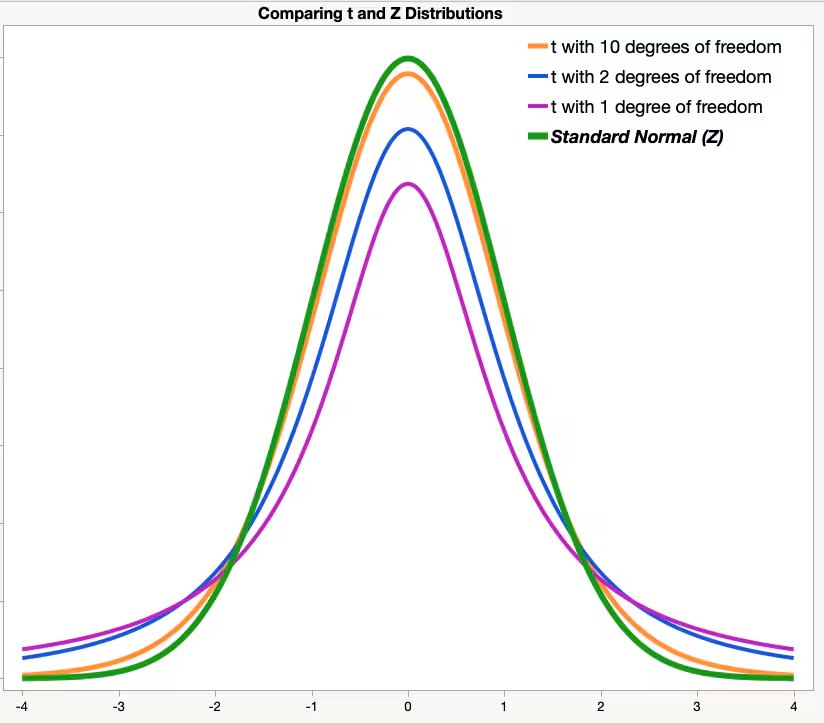
\includegraphics[width=0.7\linewidth,height=\textheight,keepaspectratio]{images/t_distribution.png}

}

\caption{\label{fig-t}Examples of heavy-tailed distributions.}

\end{figure}%

{\(t\)-distribution} has \emph{higher} kurtosis than normal
distributions.

\begin{itemize}
\tightlist
\item
  Meaning that \(t\)-distribution has a higher probability of obtaining
  values that are far from the mean than a normal distribution.
\item
  It is less peaked in the center and higher in the tails than normal
  distribution.
\item
  As the degree of freedom increases, \(t\)-distribution approximates to
  normal distribution, kurtosis decreases and approximates to 3.
\end{itemize}

\begin{figure}[H]

\centering{

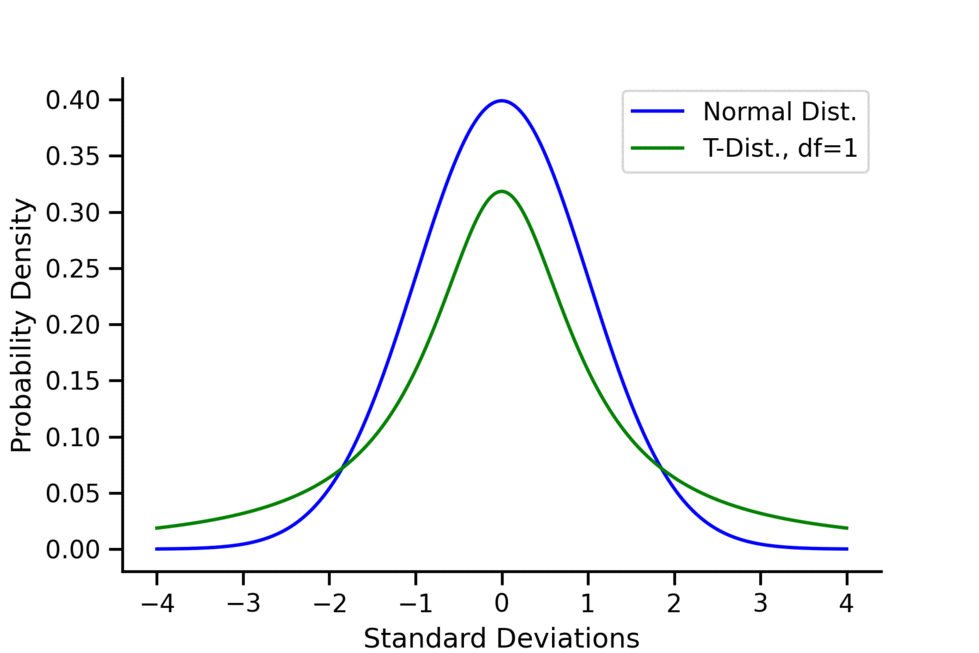
\includegraphics[width=0.8\linewidth,height=\textheight,keepaspectratio]{images/t-dist_chang_df_static.png}

}

\caption{\label{fig-t-dist-change-df}The comparison between the
\emph{t}-distribution and the normal distribution at degrees of freedom
ranging from 1 to 50. Figure source: from
\href{https://tjkyner.medium.com/the-normal-distribution-vs-students-t-distribution-322aa12ffd15}{T.J.
Kyner}.}

\end{figure}%

\begin{tcolorbox}[enhanced jigsaw, colframe=quarto-callout-tip-color-frame, colback=white, opacityback=0, breakable, coltitle=black, opacitybacktitle=0.6, toptitle=1mm, colbacktitle=quarto-callout-tip-color!10!white, arc=.35mm, bottomtitle=1mm, titlerule=0mm, toprule=.15mm, title=\textcolor{quarto-callout-tip-color}{\faLightbulb}\hspace{0.5em}{For the \(t\)-distribution:}, leftrule=.75mm, rightrule=.15mm, left=2mm, bottomrule=.15mm]

\begin{itemize}
\tightlist
\item
  As the degrees of freedom (df) increase, the \(t\)-distribution
  approaches the normal distribution.
\item
  A common rule of thumb is that for \(df > 30\), one can pretty safely
  use the normal distribution in place of a \emph{t}-distribution unless
  you are interested in the extreme tails.
\end{itemize}

\end{tcolorbox}

Let \(\mu_4 = E[(X-\mathbb{E}[X])^4]\) be the fourth central moment.
Standardized (population) kurtosis:
\[\kappa = \frac{\mu_4}{\text{sd}(X)^4}, \qquad \text{Excess kurtosis} = \kappa - 3.\]
Sample (Fisher) excess kurtosis estimator:
\[\hat{g}_2 = \frac{n(n+1)}{(n-1)(n-2)(n-3)} \sum_{i=1}^n \left(\frac{X_i-\bar{X}}{s}\right)^4 - \frac{3(n-1)^2}{(n-2)(n-3)}.\]
High excess kurtosis signals greater tail risk; low or negative excess
indicates fewer extreme outcomes.

Interpretation link: High positive skewness without high kurtosis means
upside spikes with limited extra tail risk; high kurtosis (regardless of
skew sign) means fatter tails and a need to focus on outlier management.

\begin{example}[]\protect\hypertarget{exm-5}{}\label{exm-5}

A company's quarterly profits have excess kurtosis of 4. What does this
mean for risk management?

\end{example}

Solution

\begin{refsolution}
Excess kurtosis is defined relative to a normal distribution (which has
kurtosis 3).

\begin{itemize}
\tightlist
\item
  Excess kurtosis = Kurtosis − 3
\item
  So an excess kurtosis of 4 means the total kurtosis is \textbf{7},
  much higher than a normal distribution.
\end{itemize}

This implies the distribution of quarterly profits has \textbf{fat
tails} --- extreme profit or loss outcomes are more likely than under a
normal distribution. Recommend to focus risk management on outliers.

\label{sol-5}

\end{refsolution}

\section{Covariance, Correlation \&
Independence}\label{covariance-correlation-independence}

Population covariance measures the direction of comovement between two
variables:

\begin{itemize}
\tightlist
\item
  \textbf{Positive covariance:} Both variables increase or decrease
  together
\item
  \textbf{Negative covariance:} One increases while the other decreases
\item
  \textbf{Magnitude:} Does not indicate strength of relationship
\end{itemize}

\textbf{Population formulas:}
\[\text{Cov}(X, Y) = E[(X - E[X])(Y - E[Y])]\]
\[\text{Cov}(X, Y) = E[XY] - E[X]E[Y]\]

\textbf{Sample covariance (unbiased):}
\[s_{XY} = \frac{1}{n-1}\sum_{i=1}^n (X_i - \bar{X})(Y_i - \bar{Y}).\]

Population correlation standardizes covariance to a scale from -1 to 1:
\[\text{Corr}(X, Y) = \frac{\text{Cov}(X, Y)}{\text{sd}(X) \cdot \text{sd}(Y)}\]

\textbf{Sample correlation:} \[r_{XY} = \frac{s_{XY}}{s_X s_Y}.\]

\begin{itemize}
\tightlist
\item
  \textbf{Correlation = 1:} Perfect positive relationship
\item
  \textbf{Correlation = \(-1\):} Perfect negative relationship
\item
  \textbf{Correlation = 0:} No linear relationship
\end{itemize}

Independence means knowing one event doesn't affect the other:
\[P(A \text{ and } B) = P(A) \cdot P(B)\]

\begin{tcolorbox}[enhanced jigsaw, colframe=quarto-callout-caution-color-frame, colback=white, opacityback=0, breakable, coltitle=black, opacitybacktitle=0.6, toptitle=1mm, colbacktitle=quarto-callout-caution-color!10!white, arc=.35mm, bottomtitle=1mm, titlerule=0mm, toprule=.15mm, title=\textcolor{quarto-callout-caution-color}{\faFire}\hspace{0.5em}{Independence vs.~Correlation}, leftrule=.75mm, rightrule=.15mm, left=2mm, bottomrule=.15mm]

Independence means no influence between events, while correlation
measures linear relationship strength.

Independence implies zero correlation, but zero correlation does not
imply independence.

E.g., \(X\) and \(Y = X^2\) have zero correlation but are not
independent.

\end{tcolorbox}

\textbf{Business Example:} Suppose a retailer finds that sales and
weather are correlated. This information can be used to adjust inventory
planning for seasonal effects. If two marketing campaigns are
independent, the outcome of one does not affect the other.

\begin{example}[]\protect\hypertarget{exm-independence-supermarket}{}\label{exm-independence-supermarket}

Suppose a customer visits a supermarket. Let:

\begin{itemize}
\tightlist
\item
  \(A\) = ``customer buys a loaf of bread today'' and \(P(A)=30\%\).
\item
  \(B\) = ``customer buys laundry detergent today'' and \(P(B)=10\%\).
\end{itemize}

What is the probability the customer buys both bread and detergent
today? What does observing a bread purchase tell you about \(P(B)\)?

\end{example}

Solution

\begin{refsolution}
Bread (frequent staple) and detergent (infrequent refill) decisions are
unrelated, so it is reasonable to assume independence. Hence \[
P(A \text{ and } B) = 30\% \times 10\% = 3\%
\] Observing bread does not change \(P(B)=10\%\).

\label{sol-independence-supermarket}

\end{refsolution}

\begin{example}[]\protect\hypertarget{exm-7}{}\label{exm-7}

If the correlation between two stocks is \(-0.8,\) what does this mean
for portfolio diversification?

\end{example}

Solution

\begin{refsolution}
\leavevmode

They tend to move in opposite directions, aiding diversification and
reducing portfolio variance.

\label{sol-7}

\end{refsolution}

\begin{tcolorbox}[enhanced jigsaw, colframe=quarto-callout-caution-color-frame, colback=white, opacityback=0, breakable, coltitle=black, opacitybacktitle=0.6, toptitle=1mm, colbacktitle=quarto-callout-caution-color!10!white, arc=.35mm, bottomtitle=1mm, titlerule=0mm, toprule=.15mm, title=\textcolor{quarto-callout-caution-color}{\faFire}\hspace{0.5em}{Mutually Exclusive vs Independence}, leftrule=.75mm, rightrule=.15mm, left=2mm, bottomrule=.15mm]

\textbf{Mutually exclusive:} Cannot happen together \[P(A\cap B)=0\]

\textbf{Independent:} Knowledge of one does not change probability of
the other \[P(A\cap B)=P(A)P(B)\]

Think: Disjoint = ``never together''; Independent = ``no influence''.

\end{tcolorbox}

\section{Population vs.~Sample: Summary \&
Estimators}\label{population-vs.-sample-summary-estimators}

When analysing data we distinguish between:

\begin{itemize}
\tightlist
\item
  \textbf{Population parameters (target):} Fixed (but usually unknown)
  numerical characteristics of the underlying process (e.g.,
  \(\mathbb{E}[X], \text{Var}(X), \gamma_1, \kappa, \text{Cov}(X,Y)\)).
\item
  \textbf{Sample statistics (estimators):} Functions of observed data
  used to approximate population parameters (e.g.,
  \(\bar{X}, s^2, s, \hat{\gamma}_1, \hat{g}_2, s_{XY}, r_{XY}\)). They
  vary from sample to sample.
\end{itemize}

Key principles:

\begin{enumerate}
\def\labelenumi{\arabic{enumi}.}
\tightlist
\item
  Replace integrals / probability-weighted sums with empirical averages.
\item
  Center around the sample mean when the population mean is unknown.
\item
  Use \(n-1\) (unbiased) denominators for second moments (variance,
  covariance) when estimating from an i.i.d. sample.
\item
  Always interpret sample statistics as \textbf{estimates} with sampling
  variability; risk management and forecasting should account for
  estimation error (e.g., standard deviation and confidence intervals).
\end{enumerate}

\subsection{Quick Reference Table}\label{quick-reference-table}

\begin{longtable}[]{@{}
  >{\raggedright\arraybackslash}p{(\linewidth - 6\tabcolsep) * \real{0.1364}}
  >{\raggedright\arraybackslash}p{(\linewidth - 6\tabcolsep) * \real{0.4848}}
  >{\raggedright\arraybackslash}p{(\linewidth - 6\tabcolsep) * \real{0.2727}}
  >{\raggedright\arraybackslash}p{(\linewidth - 6\tabcolsep) * \real{0.1061}}@{}}
\toprule\noalign{}
\begin{minipage}[b]{\linewidth}\raggedright
Concept
\end{minipage} & \begin{minipage}[b]{\linewidth}\raggedright
Population Symbol / Definition
\end{minipage} & \begin{minipage}[b]{\linewidth}\raggedright
Sample Estimator
\end{minipage} & \begin{minipage}[b]{\linewidth}\raggedright
Notes
\end{minipage} \\
\midrule\noalign{}
\endhead
\bottomrule\noalign{}
\endlastfoot
Mean & \(\mathbb{E}[X]\) & \(\bar{X}=\tfrac{1}{n}\sum X_i\) & Unbiased
for mean (i.i.d.) \\
Variance & \(\text{Var}(X)=E[(X-\mathbb{E}[X])^2]\) &
\(s^2=\tfrac{1}{n-1}\sum (X_i-\bar{X})^2\) & \(s_n^2\) (divide by \(n\))
is biased low \\
Std. Dev. & \(\text{sd}(X)=\sqrt{\text{Var}(X)}\) & \(s=\sqrt{s^2}\) &
Plug-in \\
Skewness & \(\gamma_1=\mu_3/\text{sd}^3\),
\(\mu_3=E[(X-\mathbb{E}[X])^3]\) &
\(\hat{\gamma}_1=\frac{n}{(n-1)(n-2)}\sum (\frac{X_i-\bar{X}}{s})^3\) &
Measures asymmetry \\
Kurtosis (excess) & \(\kappa-3\), \(\kappa=\mu_4/\text{sd}^4\) &
\(\hat{g}_2\) (Fisher) & Tail heaviness vs.~normal \\
Covariance & \(\text{Cov}(X,Y)=E[(X-\mathbb{E}X)(Y-\mathbb{E}Y)]\) &
\(s_{XY}=\tfrac{1}{n-1}\sum (X_i-\bar{X})(Y_i-\bar{Y})\) & Sign =
direction \\
Correlation & \(\rho=\dfrac{\text{Cov}(X,Y)}{\text{sd}(X)\text{sd}(Y)}\)
& \(r_{XY}=\dfrac{s_{XY}}{s_X s_Y}\) & Scale-free ( -1 to 1 ) \\
\end{longtable}

\begin{tcolorbox}[enhanced jigsaw, colframe=quarto-callout-tip-color-frame, colback=white, opacityback=0, breakable, coltitle=black, opacitybacktitle=0.6, toptitle=1mm, colbacktitle=quarto-callout-tip-color!10!white, arc=.35mm, bottomtitle=1mm, titlerule=0mm, toprule=.15mm, title=\textcolor{quarto-callout-tip-color}{\faLightbulb}\hspace{0.5em}{Interpretation tip}, leftrule=.75mm, rightrule=.15mm, left=2mm, bottomrule=.15mm]

If a sample statistic looks extreme (e.g., very high skewness or
kurtosis), examine sample size and outliers; small samples amplify noise
in higher-moment estimates.

\end{tcolorbox}

\chapter{Lab 1: Probability \& Descriptive
Statistics}\label{lab-1-probability-descriptive-statistics}

\section{Instructions}\label{instructions}

Open in Google Colab:
\href{https://colab.research.google.com/drive/1JLABtp6OJUJHmODRHpQ9FQXovp73na_9?usp=share_link}{Link}

Alternatively, copy and paste the code below into RStuido Desktop or
RStudio Cloud.

Finish Quiz for Lab 1 on Canvas.

Focus: explore core descriptive statistics and dependence concepts using
simple synthetic data.

You will:

\begin{itemize}
\tightlist
\item
  Examine independence \& correlation
\item
  Compare skewed and roughly normal distributions
\item
  Compute mean, variance, sd, skewness, kurtosis
\item
  Compare biased vs unbiased variance estimators
\item
  Simulate a high-correlation (ρ = 0.90) two-asset return setting
\item
  Study sampling distributions of asset and portfolio means
\end{itemize}

\section{Datasets}\label{datasets}

Synthetic generators used:

\begin{itemize}
\tightlist
\item
  Right-skewed transaction values (log-normal)and approx. normal
  reference sample
\item
  Two correlated asset return series (ρ = 0.90) for sampling exercises
\end{itemize}

Run each cell sequentially. Read the comments carefully.

\begin{Shaded}
\begin{Highlighting}[]
\CommentTok{\# {-}{-}{-}{-}{-}{-}{-}{-} Setup: packages {-}{-}{-}{-}{-}{-}{-}{-}}
\CommentTok{\# Unified required package list}
\NormalTok{pkgs }\OtherTok{\textless{}{-}} \FunctionTok{c}\NormalTok{(}\StringTok{"tidyverse"}\NormalTok{, }\StringTok{"data.table"}\NormalTok{, }\StringTok{"ggsci"}\NormalTok{, }\StringTok{"moments"}\NormalTok{, }\StringTok{"knitr"}\NormalTok{, }\StringTok{"kableExtra"}\NormalTok{, }\StringTok{"IRdisplay"}\NormalTok{)}
\NormalTok{missing }\OtherTok{\textless{}{-}} \FunctionTok{setdiff}\NormalTok{(pkgs, }\FunctionTok{rownames}\NormalTok{(}\FunctionTok{installed.packages}\NormalTok{()))}
\ControlFlowTok{if}\NormalTok{ (}\FunctionTok{length}\NormalTok{(missing) }\SpecialCharTok{\textgreater{}} \DecValTok{0}\NormalTok{) }\FunctionTok{install.packages}\NormalTok{(missing)}

\CommentTok{\# Load all packages (silently)}
\FunctionTok{invisible}\NormalTok{(}\FunctionTok{lapply}\NormalTok{(pkgs, }\ControlFlowTok{function}\NormalTok{(pkg) \{}
  \FunctionTok{suppressWarnings}\NormalTok{(}\FunctionTok{suppressPackageStartupMessages}\NormalTok{(}\FunctionTok{library}\NormalTok{(pkg, }\AttributeTok{character.only =} \ConstantTok{TRUE}\NormalTok{)))}
\NormalTok{\}))}

\CommentTok{\# Set default options for figures in Jupyter Notebook}
\FunctionTok{options}\NormalTok{(}\AttributeTok{repr.plot.width =} \DecValTok{12}\NormalTok{, }\AttributeTok{repr.plot.height =} \DecValTok{4}\NormalTok{)  }\CommentTok{\# wider default figures}

\FunctionTok{message}\NormalTok{(}\StringTok{"}\SpecialCharTok{\textbackslash{}n}\StringTok{Setup complete (packages loaded: "}\NormalTok{, }\FunctionTok{paste}\NormalTok{(pkgs, }\AttributeTok{collapse =} \StringTok{", "}\NormalTok{), }\StringTok{")."}\NormalTok{)}
\end{Highlighting}
\end{Shaded}

\begin{verbatim}

Setup complete (packages loaded: tidyverse, data.table, ggsci, moments, knitr, kableExtra, IRdisplay).
\end{verbatim}

\section{Independence vs.~Zero
Correlation}\label{independence-vs.-zero-correlation}

Independence means no influence between events, while correlation
measures linear relationship strength.

Independence implies zero correlation, but zero correlation does not
imply independence.

E.g., \(X\) and \(Y = X^2\) have zero correlation but are not
independent.

\begin{Shaded}
\begin{Highlighting}[]
\CommentTok{\# {-}{-}{-}{-} Zero Correlation but NOT Independence: Y = X\^{}2 {-}{-}{-}{-}}
\CommentTok{\# Idea: X \textasciitilde{} N(0,1); define Y = X\^{}2.  Then cor(X,Y) \textasciitilde{} 0 (symmetry cancels linear relation),}
\CommentTok{\# yet Y is a deterministic function of X so they are NOT independent.}

\FunctionTok{set.seed}\NormalTok{(}\DecValTok{2025}\NormalTok{)}
\NormalTok{n }\OtherTok{\textless{}{-}} \DecValTok{5000}
\NormalTok{X }\OtherTok{\textless{}{-}} \FunctionTok{rnorm}\NormalTok{(n)}
\NormalTok{Y }\OtherTok{\textless{}{-}}\NormalTok{ X}\SpecialCharTok{\^{}}\DecValTok{2}
\NormalTok{r\_xy }\OtherTok{\textless{}{-}} \FunctionTok{cor}\NormalTok{(X, Y)}
\FunctionTok{cat}\NormalTok{(}\FunctionTok{sprintf}\NormalTok{(}\StringTok{"Sample correlation cor(X, Y=X\^{}2) = \%.4f (near 0)}\SpecialCharTok{\textbackslash{}n}\StringTok{"}\NormalTok{, r\_xy))}
\end{Highlighting}
\end{Shaded}

\begin{verbatim}
Sample correlation cor(X, Y=X^2) = 0.0198 (near 0)
\end{verbatim}

We got \(\rho_{X,Y}=0.0198\). It seems to be close to zero, but we need
a statistical test to confirm this formally.

→ Test for significance of the correlation coefficient

\begin{Shaded}
\begin{Highlighting}[]
\FunctionTok{cor.test}\NormalTok{(X, Y)}
\end{Highlighting}
\end{Shaded}

\begin{verbatim}

    Pearson's product-moment correlation

data:  X and Y
t = 1.4027, df = 4998, p-value = 0.1608
alternative hypothesis: true correlation is not equal to 0
95 percent confidence interval:
 -0.007887062  0.047529726
sample estimates:
       cor 
0.01983657 
\end{verbatim}

\begin{center}\rule{0.5\linewidth}{0.5pt}\end{center}


\includegraphics[width=\linewidth,height=1em,keepaspectratio]{filters/emoji/1f4a1.png}
\textbf{Q: Based on the output of \texttt{cor.test}, what is the p-value
for the correlation test? What can you conclude about the correlation
between the two variables?} Are \(X\) and \(Y\) independent? Write your
answer in the cell below.

A: {[}Type your answer here{]}

Distinguish the two expressions:

\begin{itemize}
\tightlist
\item
  correlation coefficient equals zero
  
\includegraphics[width=\linewidth,height=1em,keepaspectratio]{filters/emoji/274c.png}
\item
  correlation coefficient (statistically) indifferent from zero
  
\includegraphics[width=\linewidth,height=1em,keepaspectratio]{filters/emoji/2705.png}
\end{itemize}

\begin{center}\rule{0.5\linewidth}{0.5pt}\end{center}

Now let's visualize \(Y=X^2\) by plotting the scatter plot.

\begin{Shaded}
\begin{Highlighting}[]
\FunctionTok{library}\NormalTok{(ggplot2)}
\FunctionTok{options}\NormalTok{(}\AttributeTok{repr.plot.width =} \DecValTok{8}\NormalTok{, }\AttributeTok{repr.plot.height =} \DecValTok{7}\NormalTok{)}
\NormalTok{scatter\_df }\OtherTok{\textless{}{-}} \FunctionTok{data.frame}\NormalTok{(}\AttributeTok{X =}\NormalTok{ X, }\AttributeTok{Y =}\NormalTok{ Y)}
\NormalTok{p1 }\OtherTok{\textless{}{-}} \FunctionTok{ggplot}\NormalTok{(scatter\_df, }\FunctionTok{aes}\NormalTok{(X, Y)) }\SpecialCharTok{+}
  \FunctionTok{geom\_point}\NormalTok{(}\AttributeTok{alpha =} \FloatTok{0.25}\NormalTok{, }\AttributeTok{color =} \StringTok{\textquotesingle{}\#2c7fb8\textquotesingle{}}\NormalTok{) }\SpecialCharTok{+}
  \FunctionTok{annotate}\NormalTok{(}\StringTok{\textquotesingle{}text\textquotesingle{}}\NormalTok{, }\AttributeTok{x =} \FunctionTok{min}\NormalTok{(X)}\SpecialCharTok{+}\FloatTok{0.2}\NormalTok{, }\AttributeTok{y =} \FunctionTok{max}\NormalTok{(Y)}\SpecialCharTok{*}\FloatTok{0.95}\NormalTok{,}
           \AttributeTok{label =} \FunctionTok{paste0}\NormalTok{(}\StringTok{\textquotesingle{}cor = \textquotesingle{}}\NormalTok{, }\FunctionTok{sprintf}\NormalTok{(}\StringTok{\textquotesingle{}\%.3f\textquotesingle{}}\NormalTok{, r\_xy)),}
           \AttributeTok{hjust =} \DecValTok{0}\NormalTok{, }\AttributeTok{size =} \DecValTok{4}\NormalTok{) }\SpecialCharTok{+}
  \FunctionTok{labs}\NormalTok{(}\AttributeTok{title =} \StringTok{\textquotesingle{}Zero Linear Correlation but Nonlinear Dependence\textquotesingle{}}\NormalTok{,}
       \AttributeTok{subtitle =} \StringTok{\textquotesingle{}Y = X\^{}2 with X \textasciitilde{} N(0,1)\textquotesingle{}}\NormalTok{,}
       \AttributeTok{x =} \StringTok{\textquotesingle{}X\textquotesingle{}}\NormalTok{, }\AttributeTok{y =} \StringTok{\textquotesingle{}Y = X\^{}2\textquotesingle{}}\NormalTok{) }\SpecialCharTok{+}
  \FunctionTok{theme\_minimal}\NormalTok{()}
\FunctionTok{print}\NormalTok{(p1)}
\end{Highlighting}
\end{Shaded}

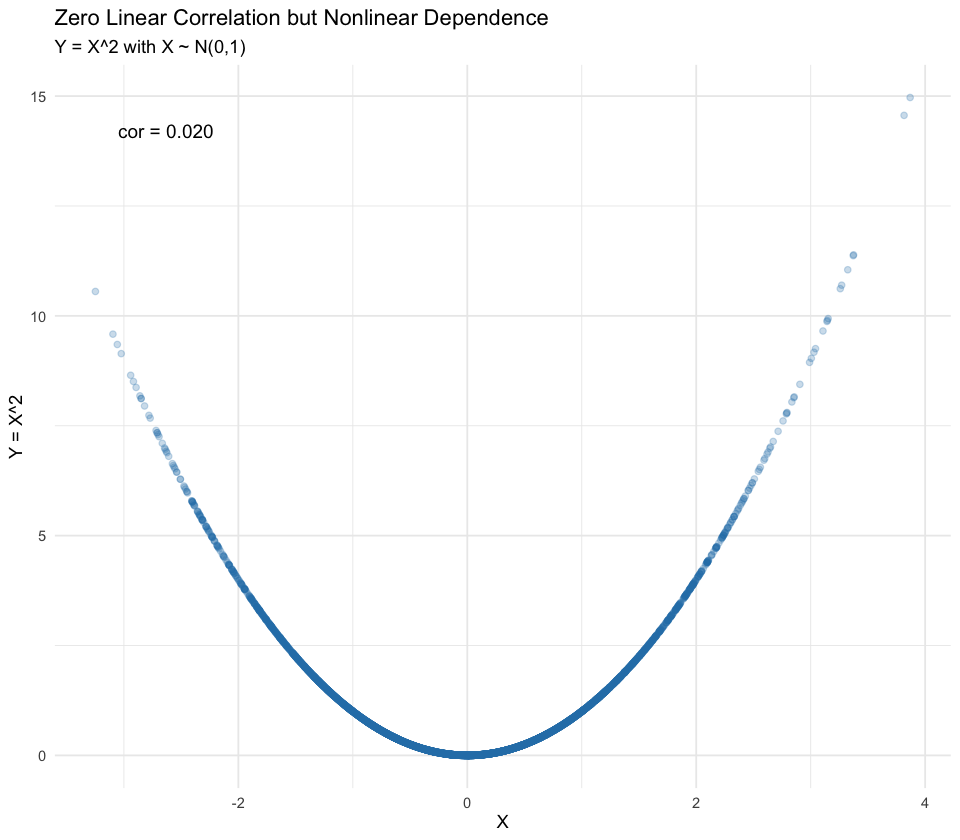
\includegraphics[width=5in,height=4.375in]{01_Lab-1_files/figure-pdf/cell-6-output-1.png}

The following figure shows the scatter plot of two assets with various
correlation coefficients.

\section{Descriptive Statistics on Asset
Returns}\label{descriptive-statistics-on-asset-returns}

\begin{Shaded}
\begin{Highlighting}[]
\CommentTok{\# {-}{-}{-}{-} Load Asset Returns Data {-}{-}{-}{-}}
\NormalTok{asset\_df }\OtherTok{\textless{}{-}} \FunctionTok{read\_csv}\NormalTok{(}\StringTok{"https://raw.githubusercontent.com/my1396/FIN5005{-}Fall2025/refs/heads/main/data/asset\_returns.csv"}\NormalTok{)}
\FunctionTok{print}\NormalTok{(}\StringTok{"Preview: first 6 rows of asset returns data frame:"}\NormalTok{)}
\FunctionTok{head}\NormalTok{(asset\_df) }\SpecialCharTok{\%\textgreater{}\%} \FunctionTok{round}\NormalTok{(}\DecValTok{2}\NormalTok{)}
\end{Highlighting}
\end{Shaded}

\begin{verbatim}
Rows: 10000 Columns: 3
── Column specification ────────────────────────────────────────────────────────
Delimiter: ","
dbl (3): Asset_A, Asset_B, Asset_C

ℹ Use `spec()` to retrieve the full column specification for this data.
ℹ Specify the column types or set `show_col_types = FALSE` to quiet this message.
\end{verbatim}

\begin{verbatim}
[1] "Preview: first 6 rows of asset returns data frame:"
\end{verbatim}

A tibble: 6 × 3

\begin{longtable}[]{@{}lll@{}}
\toprule\noalign{}
Asset\_A \textless dbl\textgreater{} & Asset\_B
\textless dbl\textgreater{} & Asset\_C \textless dbl\textgreater{} \\
\midrule\noalign{}
\endhead
\bottomrule\noalign{}
\endlastfoot
17.89 & 4.31 & 9.94 \\
10.30 & 4.17 & 10.55 \\
20.87 & 14.16 & 6.61 \\
18.21 & 22.33 & 9.58 \\
17.49 & 2.23 & 10.23 \\
29.87 & 15.72 & 8.97 \\
\end{longtable}

We define a summary statistics function to compute the statistics of
interest.

\begin{Shaded}
\begin{Highlighting}[]
\NormalTok{quick\_summary }\OtherTok{\textless{}{-}} \ControlFlowTok{function}\NormalTok{(x) \{}
  \CommentTok{\# Function to compute basic descriptive statistics}
  \FunctionTok{data.frame}\NormalTok{(}
    \AttributeTok{n =} \FunctionTok{length}\NormalTok{(x),}
    \AttributeTok{mean =} \FunctionTok{mean}\NormalTok{(x),}
    \AttributeTok{sd =} \FunctionTok{sd}\NormalTok{(x),}
    \AttributeTok{var =} \FunctionTok{var}\NormalTok{(x),}
    \AttributeTok{skewness =}\NormalTok{ moments}\SpecialCharTok{::}\FunctionTok{skewness}\NormalTok{(x),}
    \AttributeTok{kurtosis =}\NormalTok{ moments}\SpecialCharTok{::}\FunctionTok{kurtosis}\NormalTok{(x),}
    \AttributeTok{row.names =} \ConstantTok{NULL}
\NormalTok{  )}
\NormalTok{\}}
\end{Highlighting}
\end{Shaded}

The summary statistic table is generated as follows:

\begin{Shaded}
\begin{Highlighting}[]
\NormalTok{results }\OtherTok{\textless{}{-}} \FunctionTok{lapply}\NormalTok{(asset\_df, quick\_summary) }\SpecialCharTok{\%\textgreater{}\%}
    \FunctionTok{do.call}\NormalTok{(rbind, .) }\SpecialCharTok{\%\textgreater{}\%}
    \FunctionTok{kable}\NormalTok{(}\AttributeTok{format =} \StringTok{"html"}\NormalTok{, }\AttributeTok{digits =} \DecValTok{2}\NormalTok{, }\AttributeTok{caption =} \StringTok{"Descriptive Statistics of Asset Returns"}\NormalTok{)}
\FunctionTok{display\_html}\NormalTok{(}\FunctionTok{as.character}\NormalTok{(results)) }
\end{Highlighting}
\end{Shaded}

\begin{longtable}[]{@{}lrrrrrr@{}}
\caption{Descriptive Statistics of Asset Returns}\tabularnewline
\toprule\noalign{}
& n & mean & sd & var & skewness & kurtosis \\
\midrule\noalign{}
\endfirsthead
\toprule\noalign{}
& n & mean & sd & var & skewness & kurtosis \\
\midrule\noalign{}
\endhead
\bottomrule\noalign{}
\endlastfoot
Asset\_A & 10000 & 20.14 & 4.82 & 23.24 & -0.10 & 3.15 \\
Asset\_B & 10000 & 8.50 & 4.44 & 19.71 & 1.71 & 9.19 \\
Asset\_C & 10000 & 9.99 & 1.01 & 1.01 & -0.85 & 3.50 \\
\end{longtable}

Plot the histograms of the asset returns to visualize their
distributions.

\begin{Shaded}
\begin{Highlighting}[]
\CommentTok{\# {-}{-}{-}{-} Visualization: Histograms with Normal Density Overlay {-}{-}{-}{-}}
\CommentTok{\# Convert to long form}
\NormalTok{combined }\OtherTok{\textless{}{-}}\NormalTok{ asset\_df }\SpecialCharTok{\%\textgreater{}\%} \FunctionTok{pivot\_longer}\NormalTok{(}\AttributeTok{cols =} \FunctionTok{everything}\NormalTok{(), }\AttributeTok{names\_to =} \StringTok{"type"}\NormalTok{, }\AttributeTok{values\_to =} \StringTok{"value"}\NormalTok{)}

\CommentTok{\# Compute per{-}type mean \& sd and create normal curve points}
\NormalTok{norm\_params }\OtherTok{\textless{}{-}}\NormalTok{ combined }\SpecialCharTok{\%\textgreater{}\%} \FunctionTok{group\_by}\NormalTok{(type) }\SpecialCharTok{\%\textgreater{}\%} \FunctionTok{summarise}\NormalTok{(}\AttributeTok{mu =} \FunctionTok{mean}\NormalTok{(value), }\AttributeTok{sigma =} \FunctionTok{sd}\NormalTok{(value), }\AttributeTok{.groups =} \StringTok{\textquotesingle{}drop\textquotesingle{}}\NormalTok{)}

\NormalTok{norm\_curve }\OtherTok{\textless{}{-}}\NormalTok{ norm\_params }\SpecialCharTok{\%\textgreater{}\%} \FunctionTok{group\_by}\NormalTok{(type) }\SpecialCharTok{\%\textgreater{}\%} \FunctionTok{do}\NormalTok{(\{}
\NormalTok{  mu }\OtherTok{\textless{}{-}}\NormalTok{ .}\SpecialCharTok{$}\NormalTok{mu; sigma }\OtherTok{\textless{}{-}}\NormalTok{ .}\SpecialCharTok{$}\NormalTok{sigma}
\NormalTok{  x }\OtherTok{\textless{}{-}} \FunctionTok{seq}\NormalTok{(mu }\SpecialCharTok{{-}} \DecValTok{4}\SpecialCharTok{*}\NormalTok{sigma, mu }\SpecialCharTok{+} \DecValTok{4}\SpecialCharTok{*}\NormalTok{sigma, }\AttributeTok{length.out =} \DecValTok{400}\NormalTok{)}
  \FunctionTok{tibble}\NormalTok{(}\AttributeTok{value =}\NormalTok{ x, }\AttributeTok{density =} \FunctionTok{dnorm}\NormalTok{(x, mu, sigma))}
\NormalTok{\})}

\FunctionTok{options}\NormalTok{(}\AttributeTok{repr.plot.width =} \DecValTok{15}\NormalTok{, }\AttributeTok{repr.plot.height =} \DecValTok{6}\NormalTok{)}

\FunctionTok{ggplot}\NormalTok{(combined, }\FunctionTok{aes}\NormalTok{(value)) }\SpecialCharTok{+}
  \FunctionTok{geom\_histogram}\NormalTok{(}\FunctionTok{aes}\NormalTok{(}\AttributeTok{y =} \FunctionTok{after\_stat}\NormalTok{(density)), }\AttributeTok{bins =} \DecValTok{40}\NormalTok{, }\AttributeTok{fill =} \StringTok{"\#3182bd"}\NormalTok{, }\AttributeTok{alpha =} \FloatTok{0.8}\NormalTok{, }\AttributeTok{color =} \StringTok{"white"}\NormalTok{) }\SpecialCharTok{+}
  \FunctionTok{geom\_line}\NormalTok{(}\AttributeTok{data =}\NormalTok{ norm\_curve, }\FunctionTok{aes}\NormalTok{(value, density), }\AttributeTok{color =} \StringTok{"red"}\NormalTok{, }\AttributeTok{linewidth =} \FloatTok{0.8}\NormalTok{) }\SpecialCharTok{+}
  \FunctionTok{facet\_wrap}\NormalTok{(}\SpecialCharTok{\textasciitilde{}}\NormalTok{ type, }\AttributeTok{scales =} \StringTok{"free"}\NormalTok{, }\AttributeTok{nrow =} \DecValTok{1}\NormalTok{) }\SpecialCharTok{+}
  \FunctionTok{labs}\NormalTok{(}\AttributeTok{title =} \StringTok{"Distribution Contrast with Normal Overlay"}\NormalTok{,}
       \AttributeTok{subtitle =} \StringTok{"Red curve = fitted normal using sample mean \& sd per asset"}\NormalTok{,}
       \AttributeTok{x =} \StringTok{"Value"}\NormalTok{, }\AttributeTok{y =} \StringTok{"Density"}\NormalTok{) }\SpecialCharTok{+}
  \FunctionTok{theme}\NormalTok{(}\AttributeTok{panel.spacing.x =} \FunctionTok{unit}\NormalTok{(}\FloatTok{1.2}\NormalTok{, }\StringTok{"lines"}\NormalTok{))}
\end{Highlighting}
\end{Shaded}

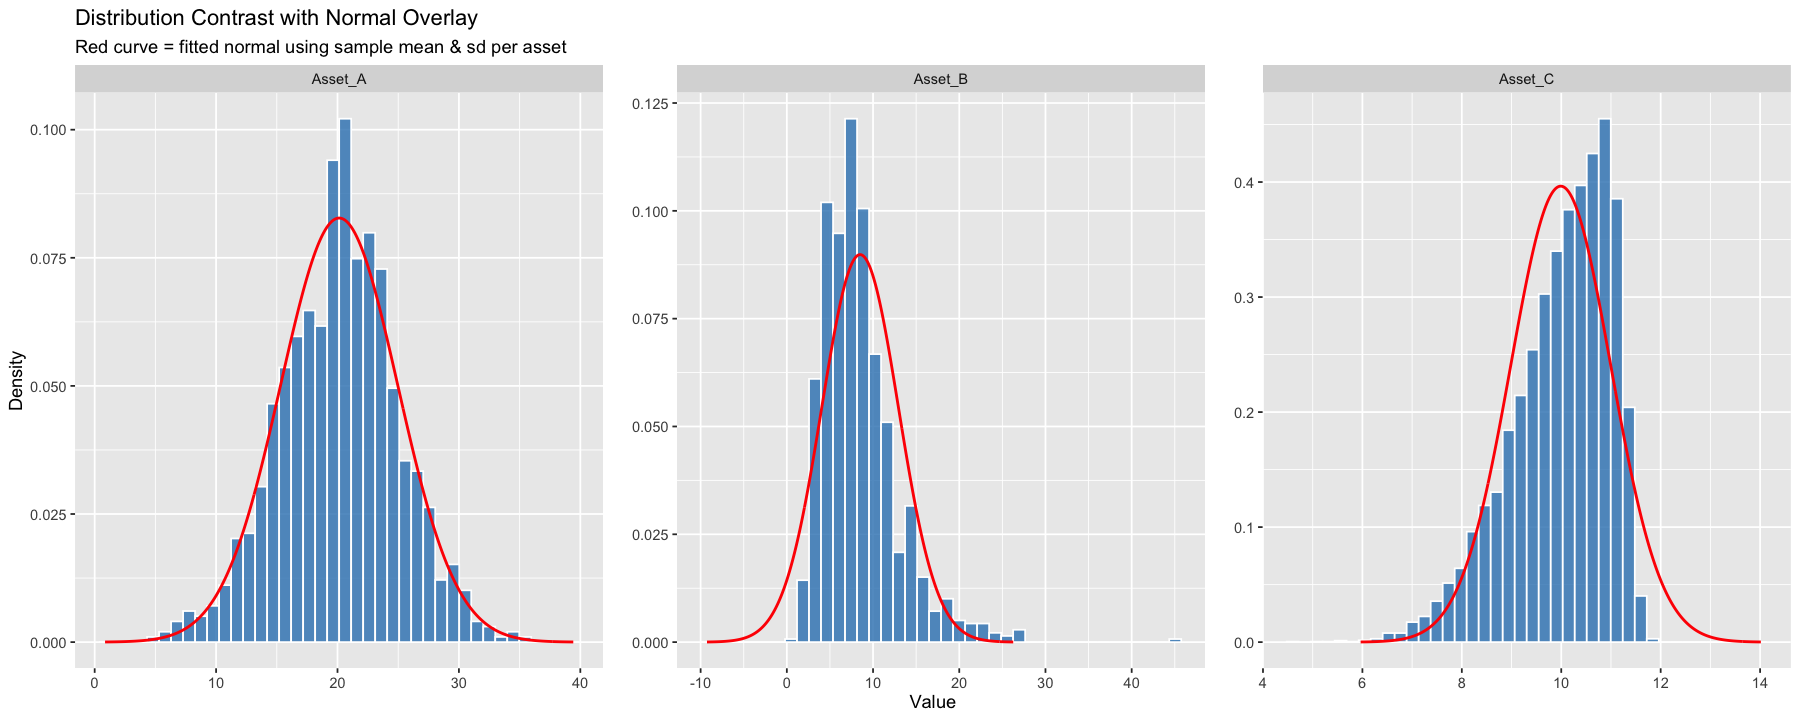
\includegraphics[width=9.375in,height=3.75in]{01_Lab-1_files/figure-pdf/cell-10-output-1.png}

\begin{center}\rule{0.5\linewidth}{0.5pt}\end{center}


\includegraphics[width=\linewidth,height=1em,keepaspectratio]{filters/emoji/1f4a1.png}
\textbf{Q: Answer the following questions based on the summary
statistics and the distribution plots:}

\begin{itemize}
\tightlist
\item
  Which asset has the highest mean return?
\item
  Which asset is the most risky? and which one has the most stable
  returns?
\item
  Which asset shows the positive skewness and what does it mean?
\item
  If an investor prefers assets with low risk and return distributions
  with tails close to normal, which asset is most appropriate?
\item
  Based on mean and standard deviation, which asset has the best
  risk--return trade-off (highest mean per unit of risk)?
\end{itemize}

A: {[}Type your answer here{]}

\begin{center}\rule{0.5\linewidth}{0.5pt}\end{center}

\section{Large Sample Gives More Accurate
Estimates}\label{large-sample-gives-more-accurate-estimates}

We have a variable \(X\sim N(0,5^2).\)

Normal distribution notation: \(X\sim N(\mu, \sigma^2)\) means that
\(X\) is normally distributed with mean \(\mu\) and variance
\(\sigma^2.\)

The second parameter is the variance, \textbf{NOT} the standard
deviation.

Now we draw random samples of size 5, 10, 10, \ldots{} until 5000 from
this distribution and compute the sample mean and standard deviation for
each sample.

For each sample, we compute the biased and unbiased sample variance

\begin{itemize}
\tightlist
\item
  The biased sample variance is computed as
  \[\frac{1}{n}\sum_{i=1}^n (x_i - \bar{x})^2.\]
\item
  The unbiased sample variance is computed as
  \[\frac{1}{n-1}\sum_{i=1}^n (x_i - \bar{x})^2\]
\end{itemize}

\begin{Shaded}
\begin{Highlighting}[]
\CommentTok{\# {-}{-}{-}{-} Simulation: Sample vs Population variance {-}{-}{-}{-}}
\FunctionTok{set.seed}\NormalTok{(}\DecValTok{2025}\NormalTok{)  }\CommentTok{\# for reproducibility}
\NormalTok{true\_var }\OtherTok{\textless{}{-}} \DecValTok{25}  \CommentTok{\# sd\^{}2 with sd=5, true population variance}
\NormalTok{sample\_sizes }\OtherTok{\textless{}{-}} \FunctionTok{c}\NormalTok{(}\DecValTok{5}\NormalTok{, }\DecValTok{10}\NormalTok{, }\DecValTok{20}\NormalTok{, }\DecValTok{50}\NormalTok{, }\DecValTok{100}\NormalTok{, }\DecValTok{250}\NormalTok{, }\DecValTok{500}\NormalTok{, }\DecValTok{1000}\NormalTok{, }\DecValTok{5000}\NormalTok{) }\CommentTok{\# varying sample sizes from 5 to 500}
\NormalTok{results }\OtherTok{\textless{}{-}} \FunctionTok{lapply}\NormalTok{(sample\_sizes, }\ControlFlowTok{function}\NormalTok{(n)\{}
\NormalTok{  x }\OtherTok{\textless{}{-}} \FunctionTok{rnorm}\NormalTok{(n, }\AttributeTok{mean =} \DecValTok{0}\NormalTok{, }\AttributeTok{sd =} \DecValTok{5}\NormalTok{)}
  \FunctionTok{data.frame}\NormalTok{(}\StringTok{"sample\_size"} \OtherTok{=}\NormalTok{ n, }\StringTok{"var\_biased"} \OtherTok{=} \FunctionTok{mean}\NormalTok{((x }\SpecialCharTok{{-}} \FunctionTok{mean}\NormalTok{(x))}\SpecialCharTok{\^{}}\DecValTok{2}\NormalTok{), }\StringTok{"var\_unbiased"} \OtherTok{=} \FunctionTok{var}\NormalTok{(x))}
\NormalTok{\}) }\SpecialCharTok{\%\textgreater{}\%}\NormalTok{ dplyr}\SpecialCharTok{::}\FunctionTok{bind\_rows}\NormalTok{()}
\FunctionTok{cat}\NormalTok{(}\StringTok{\textquotesingle{}Variance estimators: var\_n (biased, divide by n) vs var\_n1 (unbiased, divide by n{-}1).}\SpecialCharTok{\textbackslash{}n}\StringTok{\textquotesingle{}}\NormalTok{)}
\NormalTok{results}
\end{Highlighting}
\end{Shaded}

\begin{verbatim}
Variance estimators: var_n (biased, divide by n) vs var_n1 (unbiased, divide by n-1).
\end{verbatim}

A data.frame: 9 × 3

\begin{longtable}[]{@{}
  >{\raggedright\arraybackslash}p{(\linewidth - 4\tabcolsep) * \real{0.3333}}
  >{\raggedright\arraybackslash}p{(\linewidth - 4\tabcolsep) * \real{0.3333}}
  >{\raggedright\arraybackslash}p{(\linewidth - 4\tabcolsep) * \real{0.3333}}@{}}
\toprule\noalign{}
\begin{minipage}[b]{\linewidth}\raggedright
sample\_size \textless dbl\textgreater{}
\end{minipage} & \begin{minipage}[b]{\linewidth}\raggedright
var\_biased \textless dbl\textgreater{}
\end{minipage} & \begin{minipage}[b]{\linewidth}\raggedright
var\_unbiased \textless dbl\textgreater{}
\end{minipage} \\
\midrule\noalign{}
\endhead
\bottomrule\noalign{}
\endlastfoot
5 & 4.262707 & 5.328384 \\
10 & 14.832929 & 16.481032 \\
20 & 33.210505 & 34.958426 \\
50 & 25.332410 & 25.849398 \\
100 & 24.957059 & 25.209150 \\
250 & 22.936725 & 23.028840 \\
500 & 25.862610 & 25.914439 \\
1000 & 25.574182 & 25.599782 \\
5000 & 25.301658 & 25.306719 \\
\end{longtable}

\begin{center}\rule{0.5\linewidth}{0.5pt}\end{center}


\includegraphics[width=\linewidth,height=1em,keepaspectratio]{filters/emoji/1f4a1.png}
\textbf{Q: Based on the variance estimates for different sample sizes:}

\begin{itemize}
\tightlist
\item
  \textbf{As the sample size increases, how do the sample variance
  estimates compare to the true variance \(25\)?}
\item
  \textbf{Does the sample variance converge to the true variance as the
  sample size increases?}
\item
  \textbf{What is the difference between the biased and unbiased sample
  variance estimators?}
\end{itemize}

A: {[}Type your answer here{]}

\begin{center}\rule{0.5\linewidth}{0.5pt}\end{center}

\begin{Shaded}
\begin{Highlighting}[]
\CommentTok{\# {-}{-}{-}{-} Plot: Convergence of variance estimators {-}{-}{-}{-}}

\NormalTok{results\_long }\OtherTok{\textless{}{-}}\NormalTok{ results }\SpecialCharTok{\%\textgreater{}\%}
\NormalTok{  tidyr}\SpecialCharTok{::}\FunctionTok{pivot\_longer}\NormalTok{(var\_biased}\SpecialCharTok{:}\NormalTok{var\_unbiased, }\AttributeTok{names\_to =} \StringTok{"estimator"}\NormalTok{, }\AttributeTok{values\_to =} \StringTok{"value"}\NormalTok{) }\SpecialCharTok{\%\textgreater{}\%}
\NormalTok{  dplyr}\SpecialCharTok{::}\FunctionTok{mutate}\NormalTok{(}\AttributeTok{estimator =}\NormalTok{ dplyr}\SpecialCharTok{::}\FunctionTok{recode}\NormalTok{(estimator, }\AttributeTok{var\_n =} \StringTok{"Divide by n"}\NormalTok{, }\AttributeTok{var\_n1 =} \StringTok{"Divide by n{-}1"}\NormalTok{))}

\NormalTok{p }\OtherTok{\textless{}{-}} \FunctionTok{ggplot}\NormalTok{(results\_long, }\FunctionTok{aes}\NormalTok{(sample\_size, value, }\AttributeTok{color =}\NormalTok{ estimator)) }\SpecialCharTok{+}
  \FunctionTok{geom\_line}\NormalTok{() }\SpecialCharTok{+}
  \FunctionTok{geom\_point}\NormalTok{() }\SpecialCharTok{+}
  \FunctionTok{scale\_color\_npg}\NormalTok{() }\SpecialCharTok{+}
  \FunctionTok{geom\_hline}\NormalTok{(}\AttributeTok{yintercept =}\NormalTok{ true\_var, }\AttributeTok{linetype =} \StringTok{"dashed"}\NormalTok{) }\SpecialCharTok{+}
  \FunctionTok{xlim}\NormalTok{(}\FunctionTok{c}\NormalTok{(}\DecValTok{0}\NormalTok{,}\DecValTok{500}\NormalTok{)) }\SpecialCharTok{+}
  \FunctionTok{labs}\NormalTok{(}\AttributeTok{title =} \StringTok{"Convergence of Variance Estimators"}\NormalTok{, }\AttributeTok{y =} \StringTok{"Estimated variance"}\NormalTok{, }\AttributeTok{x =} \StringTok{"Sample size"}\NormalTok{) }\SpecialCharTok{+}
  \FunctionTok{theme\_bw}\NormalTok{(}\AttributeTok{base\_size =} \DecValTok{16}\NormalTok{)}
\NormalTok{p}
\end{Highlighting}
\end{Shaded}

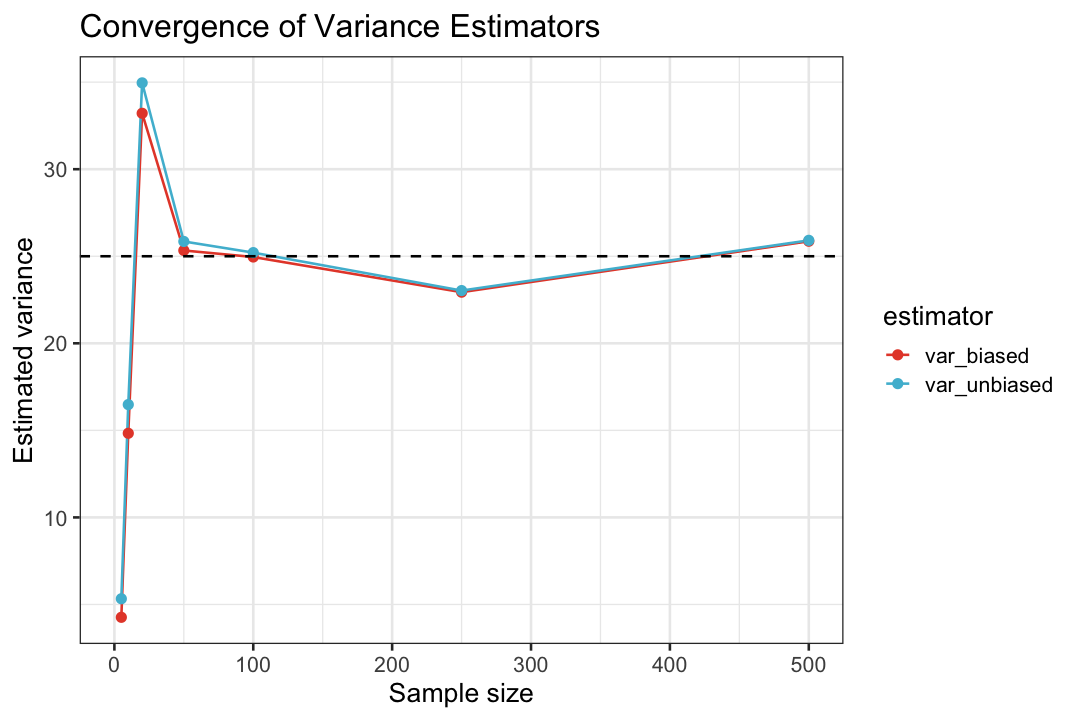
\includegraphics[width=5.625in,height=3.75in]{01_Lab-1_files/figure-pdf/cell-12-output-1.png}

\section{Correlated Asset Returns}\label{correlated-asset-returns}

We will simulate repeated samples of two (correlated) asset return
series and compare the sampling distributions of their sample means and
the distribution of the portfolio mean (equal weights).

\begin{Shaded}
\begin{Highlighting}[]
\CommentTok{\# {-}{-}{-}{-} Load Correlated Asset Returns Data {-}{-}{-}{-}}
\NormalTok{X\_demo }\OtherTok{\textless{}{-}} \FunctionTok{read\_csv}\NormalTok{(}\StringTok{"https://raw.githubusercontent.com/my1396/FIN5005{-}Fall2025/refs/heads/main/data/correlated\_asset\_returns.csv"}\NormalTok{)}
\FunctionTok{colnames}\NormalTok{(X\_demo) }\OtherTok{\textless{}{-}} \FunctionTok{c}\NormalTok{(}\StringTok{"Asset\_A"}\NormalTok{, }\StringTok{"Asset\_B"}\NormalTok{)  }\CommentTok{\# Rename columns for clarity}
\NormalTok{X\_demo }\SpecialCharTok{\%\textgreater{}\%}
    \FunctionTok{as.data.table}\NormalTok{() }\SpecialCharTok{\%\textgreater{}\%}
\NormalTok{    .[, }\FunctionTok{lapply}\NormalTok{(.SD, }\ControlFlowTok{function}\NormalTok{(x) }\ControlFlowTok{if}\NormalTok{ (}\FunctionTok{is.numeric}\NormalTok{(x)) }\FunctionTok{round}\NormalTok{(x, }\DecValTok{4}\NormalTok{) }\ControlFlowTok{else}\NormalTok{ x)] }\SpecialCharTok{\%\textgreater{}\%}
    \FunctionTok{print}\NormalTok{(}\AttributeTok{digits =} \DecValTok{4}\NormalTok{)}
\end{Highlighting}
\end{Shaded}

\begin{verbatim}
Rows: 2000 Columns: 2
── Column specification ────────────────────────────────────────────────────────
Delimiter: ","
dbl (2): V1, V2

ℹ Use `spec()` to retrieve the full column specification for this data.
ℹ Specify the column types or set `show_col_types = FALSE` to quiet this message.
\end{verbatim}

\begin{verbatim}
      Asset_A Asset_B
        <num>   <num>
   1:  0.0129  0.0351
   2:  0.0012  0.0094
   3:  0.0160  0.0130
   4:  0.0259  0.0550
   5:  0.0079  0.0147
  ---                
1996:  0.0080  0.0177
1997:  0.0061 -0.0001
1998: -0.0299 -0.0425
1999: -0.0202 -0.0357
2000:  0.0603  0.0746
\end{verbatim}

\begin{Shaded}
\begin{Highlighting}[]
\NormalTok{emp\_cor }\OtherTok{\textless{}{-}} \FunctionTok{cor}\NormalTok{(X\_demo)}
\NormalTok{emp\_cor}
\end{Highlighting}
\end{Shaded}

A matrix: 2 × 2 of type dbl

\begin{longtable}[]{@{}lll@{}}
\toprule\noalign{}
& Asset\_A & Asset\_B \\
\midrule\noalign{}
\endhead
\bottomrule\noalign{}
\endlastfoot
Asset\_A & 1.0000000 & 0.9040318 \\
Asset\_B & 0.9040318 & 1.0000000 \\
\end{longtable}

Plot the scatter plot of the two asset returns to visualize their
relationship.

\begin{Shaded}
\begin{Highlighting}[]
\FunctionTok{options}\NormalTok{(}\AttributeTok{repr.plot.width =} \DecValTok{8}\NormalTok{, }\AttributeTok{repr.plot.height =} \DecValTok{7}\NormalTok{)}
\FunctionTok{ggplot}\NormalTok{(X\_demo, }\FunctionTok{aes}\NormalTok{(Asset\_A, Asset\_B)) }\SpecialCharTok{+}
  \FunctionTok{geom\_point}\NormalTok{(}\AttributeTok{alpha =} \FloatTok{0.35}\NormalTok{, }\AttributeTok{color =} \StringTok{\textquotesingle{}\#1b7837\textquotesingle{}}\NormalTok{) }\SpecialCharTok{+}
  \FunctionTok{theme\_bw}\NormalTok{(}\AttributeTok{base\_size =} \DecValTok{16}\NormalTok{)}
\end{Highlighting}
\end{Shaded}

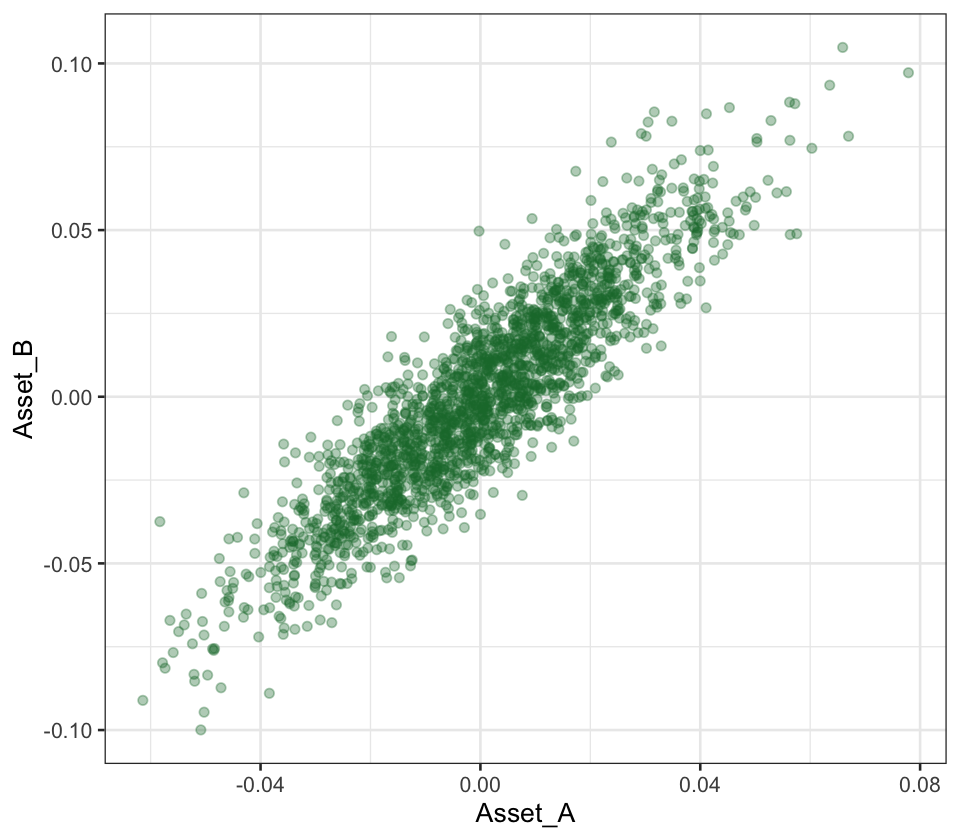
\includegraphics[width=5in,height=4.375in]{01_Lab-1_files/figure-pdf/cell-15-output-1.png}

\begin{center}\rule{0.5\linewidth}{0.5pt}\end{center}


\includegraphics[width=\linewidth,height=1em,keepaspectratio]{filters/emoji/1f4a1.png}\textbf{Q:
What is the correlation between the two asset returns? How do their
prices move together?}

A: {[}Type your answer here{]}

\begin{center}\rule{0.5\linewidth}{0.5pt}\end{center}

\subsubsection{\texorpdfstring{{ Exercise}}{ Exercise}}\label{exercise}

Following the steps below, you will compute the mean and standard
deviation of the two asset returns, construct a portfolio, and analyze
its properties.

Step 1: Calculate the standard deviation of Asset A and B returns,
respectively.

Step 2: Construct a equally weighted portfolio of the two assets.
Calculate the portfolio returns. \[
E[r_p] = \frac{1}{2} (E[r_A] + E[r_B])
\]

Step 3: Calculate the standard deviation of the portfolio returns,
\(\text{sd}(r_p)\).

Step 4: Calculate the average of the volatility of Asset A and B (using
results in Step 1). Compare it with the volatility of the portfolio
returns.

\subsection{Reflection}\label{reflection}

How does correlation between assets influence the portfolio mean's
variability? Write 3--4 sentences interpreting for a diversified vs
concentrated investment decision.

\chapter{Data Visualization}\label{data-visualization}

\begin{tcolorbox}[enhanced jigsaw, colframe=quarto-callout-note-color-frame, colback=white, opacityback=0, breakable, toprule=.15mm, arc=.35mm, leftrule=.75mm, rightrule=.15mm, left=2mm, bottomrule=.15mm]


\includegraphics[width=\linewidth,height=1em,keepaspectratio]{filters/emoji/1f3af.png}
\textbf{Study Objectives}

\begin{itemize}
\tightlist
\item
  Loads and prepares the California school dataset (CASchools) for
  analysis.

  \begin{itemize}
  \tightlist
  \item
    Demonstrates how to visualize data using scatter plots, line charts,
    histograms, box plots.
  \item
    Explores expenditure per student across different grade spans.
  \item
    Investigates correlations between expenditure and other variables.
  \end{itemize}
\item
  QQ plots to assess normality and interpret skewness and kurtosis in
  the data.

  \begin{itemize}
  \tightlist
  \item
    Given a QQ plot, you should be able to identify how does the
    distribution compare to normal: positively skewed, negatively
    skewed, has fat tails, or thin tails.
  \end{itemize}
\end{itemize}

\end{tcolorbox}

\section{\texorpdfstring{Descriptive Analysis and Data Visualization
with
\texttt{CASchools}}{Descriptive Analysis and Data Visualization with CASchools}}\label{descriptive-analysis-and-data-visualization-with-caschools}

Data visualization is a powerful tool for understanding patterns,
relationships, and distributions in datasets. In this session, we will
explore the California Schools dataset using various visualization
techniques including histograms, box plots, scatter plots, and Q-Q
plots. These visualizations help us answer important questions about
educational spending, student performance, and the relationships between
various school characteristics.

\subsection{Dataset Overview}\label{dataset-overview}

The following prints the first and last 5 rows of the dataset, together
with data types of each column:

\begin{Shaded}
\begin{Highlighting}[]
\CommentTok{\# load packages and dataset}
\NormalTok{pkgs }\OtherTok{\textless{}{-}} \FunctionTok{c}\NormalTok{(}\StringTok{"tidyverse"}\NormalTok{, }\StringTok{"moments"}\NormalTok{, }\StringTok{"data.table"}\NormalTok{, }\StringTok{"ggsci"}\NormalTok{)}
\NormalTok{missing }\OtherTok{\textless{}{-}} \FunctionTok{setdiff}\NormalTok{(pkgs, }\FunctionTok{rownames}\NormalTok{(}\FunctionTok{installed.packages}\NormalTok{()))}
\ControlFlowTok{if}\NormalTok{ (}\FunctionTok{length}\NormalTok{(missing) }\SpecialCharTok{\textgreater{}} \DecValTok{0}\NormalTok{) }\FunctionTok{install.packages}\NormalTok{(missing)}
\FunctionTok{invisible}\NormalTok{(}\FunctionTok{lapply}\NormalTok{(pkgs, }\ControlFlowTok{function}\NormalTok{(pkg) \{}
    \FunctionTok{suppressPackageStartupMessages}\NormalTok{(}\FunctionTok{library}\NormalTok{(pkg, }\AttributeTok{character.only =} \ConstantTok{TRUE}\NormalTok{))}
\NormalTok{\}))}
\NormalTok{f\_name }\OtherTok{\textless{}{-}} \StringTok{"https://raw.githubusercontent.com/my1396/FIN5005{-}Fall2025/refs/heads/main/data/CASchools\_test\_score.csv"}
\NormalTok{cas }\OtherTok{\textless{}{-}} \FunctionTok{read\_csv}\NormalTok{(f\_name, }
  \AttributeTok{col\_types =} \FunctionTok{cols}\NormalTok{(}
    \AttributeTok{county =} \FunctionTok{col\_factor}\NormalTok{(), }\CommentTok{\# read as factor}
    \AttributeTok{grades =} \FunctionTok{col\_factor}\NormalTok{()}
\NormalTok{  ))}
\end{Highlighting}
\end{Shaded}

The following prints the first and last 5 rows of the dataset, together
with data types of each column:

\begin{Shaded}
\begin{Highlighting}[]
\NormalTok{cas }\SpecialCharTok{\%\textgreater{}\%} \FunctionTok{as.data.table}\NormalTok{()}
\end{Highlighting}
\end{Shaded}

\begin{verbatim}
     district                          school      county grades students
        <num>                          <char>      <fctr> <fctr>    <num>
  1:    75119              Sunol Glen Unified     Alameda  KK-08      195
  2:    61499            Manzanita Elementary       Butte  KK-08      240
  3:    61549     Thermalito Union Elementary       Butte  KK-08     1550
  4:    61457 Golden Feather Union Elementary       Butte  KK-08      243
  5:    61523        Palermo Union Elementary       Butte  KK-08     1335
 ---                                                                     
416:    68957          Las Lomitas Elementary   San Mateo  KK-08      984
417:    69518            Los Altos Elementary Santa Clara  KK-08     3724
418:    72611          Somis Union Elementary     Ventura  KK-08      441
419:    72744               Plumas Elementary        Yuba  KK-08      101
420:    72751            Wheatland Elementary        Yuba  KK-08     1778
     teachers calworks   lunch computer expenditure    income   english  read
        <num>    <num>   <num>    <num>       <num>     <num>     <num> <num>
  1:    10.90   0.5102  2.0408       67    6384.911 22.690001  0.000000 691.6
  2:    11.15  15.4167 47.9167      101    5099.381  9.824000  4.583333 660.5
  3:    82.90  55.0323 76.3226      169    5501.955  8.978000 30.000002 636.3
  4:    14.00  36.4754 77.0492       85    7101.831  8.978000  0.000000 651.9
  5:    71.50  33.1086 78.4270      171    5235.988  9.080333 13.857677 641.8
 ---                                                                         
416:    59.73   0.1016  3.5569      195    7290.339 28.716999  5.995935 700.9
417:   208.48   1.0741  1.5038      721    5741.463 41.734108  4.726101 704.0
418:    20.15   3.5635 37.1938       45    4402.832 23.733000 24.263039 648.3
419:     5.00  11.8812 59.4059       14    4776.336  9.952000  2.970297 667.9
420:    93.40   6.9235 47.5712      313    5993.393 12.502000  5.005624 660.5
      math
     <num>
  1: 690.0
  2: 661.9
  3: 650.9
  4: 643.5
  5: 639.9
 ---      
416: 707.7
417: 709.5
418: 641.7
419: 676.5
420: 651.0
\end{verbatim}

The
\href{https://www.rdocumentation.org/packages/AER/versions/1.2-15/topics/CASchools}{\texttt{cas}}
dataset contains information on 420 public school districts in
California, specifically those that operate either kindergarten through
6th grade (K--6) or kindergarten through 8th grade (K--8) schools, with
data collected for the years 1998 and 1999.

The dataset includes:

\begin{itemize}
\tightlist
\item
  \textbf{Student performance measures} (average reading and math
  scores).
\item
  \textbf{School characteristics} (such as enrollment, number of
  teachers, student--teacher ratio, number of computers, expenditure per
  student).
\item
  \textbf{Student demographics} (including income, percentage qualifying
  for reduced-price lunch, percentage of English learners, etc.).
\end{itemize}

\texttt{cas} is a data frame containing 420 observations on 14
variables. Refer to the following table for the full definition.

\begin{longtable}[]{@{}
  >{\raggedright\arraybackslash}p{(\linewidth - 2\tabcolsep) * \real{0.1781}}
  >{\raggedright\arraybackslash}p{(\linewidth - 2\tabcolsep) * \real{0.8219}}@{}}
\toprule\noalign{}
\begin{minipage}[b]{\linewidth}\raggedright
Variable
\end{minipage} & \begin{minipage}[b]{\linewidth}\raggedright
Description
\end{minipage} \\
\midrule\noalign{}
\endhead
\bottomrule\noalign{}
\endlastfoot
\texttt{district} & Character. District code. Unique ID. \\
\texttt{school} & Character. School name. \\
\texttt{county} & Factor indicating county. \\
\texttt{grades} & Factor indicating grade span covered by the district's
schools. It takes on two values: - \texttt{KK-06}: means the district's
schools serve kindergarten through 6th grade.- \texttt{KK-08}: means the
district's schools serve kindergarten through 6th grade. \\
\texttt{students} & Total enrollment. \\
\texttt{teachers} & Number of teachers. \\
\texttt{calworks} & Percent qualifying for CalWorks (income assistance
program). \\
\texttt{lunch} & Percent qualifying for reduced-price lunch. \\
\texttt{computer} & Number of computers. \\
\texttt{expenditure} & Expenditure per student. \\
\texttt{income} & District average income (in USD 1,000). \\
\texttt{english} & Percent of English learners (i.e., students for whom
English is a second language). \\
\texttt{read} & Average reading score. \\
\texttt{math} & Average math score. \\
\end{longtable}

Data source: Stock, J. H. and Watson, M. W. (2020).
\href{https://www.sea-stat.com/wp-content/uploads/2020/08/James-H.-Stock-Mark-W.-Watson-Introduction-to-Econometrics-Global-Edition-Pearson-Education-Limited-2020.pdf}{Introduction
to Econometrics}, 4th ed.~Pearson.

\begin{center}\rule{0.5\linewidth}{0.5pt}\end{center}

\subsection{Summary Statistics}\label{summary-statistics}

The following displays the summary for each variable in the dataset:

\begin{Shaded}
\begin{Highlighting}[]
\FunctionTok{summary}\NormalTok{(cas)}
\end{Highlighting}
\end{Shaded}

\begin{verbatim}
    district        school                  county      grades   
 Min.   :61382   Length:420         Sonoma     : 29   KK-08:359  
 1st Qu.:64308   Class :character   Kern       : 27   KK-06: 61  
 Median :67760   Mode  :character   Los Angeles: 27              
 Mean   :67473                      Tulare     : 24              
 3rd Qu.:70419                      San Diego  : 21              
 Max.   :75440                      Santa Clara: 20              
                                    (Other)    :272              
    students          teachers          calworks          lunch       
 Min.   :   81.0   Min.   :   4.85   Min.   : 0.000   Min.   :  0.00  
 1st Qu.:  379.0   1st Qu.:  19.66   1st Qu.: 4.395   1st Qu.: 23.28  
 Median :  950.5   Median :  48.56   Median :10.520   Median : 41.75  
 Mean   : 2628.8   Mean   : 129.07   Mean   :13.246   Mean   : 44.71  
 3rd Qu.: 3008.0   3rd Qu.: 146.35   3rd Qu.:18.981   3rd Qu.: 66.86  
 Max.   :27176.0   Max.   :1429.00   Max.   :78.994   Max.   :100.00  
                                                                      
    computer       expenditure       income          english      
 Min.   :   0.0   Min.   :3926   Min.   : 5.335   Min.   : 0.000  
 1st Qu.:  46.0   1st Qu.:4906   1st Qu.:10.639   1st Qu.: 1.941  
 Median : 117.5   Median :5215   Median :13.728   Median : 8.778  
 Mean   : 303.4   Mean   :5312   Mean   :15.317   Mean   :15.768  
 3rd Qu.: 375.2   3rd Qu.:5601   3rd Qu.:17.629   3rd Qu.:22.970  
 Max.   :3324.0   Max.   :7712   Max.   :55.328   Max.   :85.540  
                                                                  
      read            math      
 Min.   :604.5   Min.   :605.4  
 1st Qu.:640.4   1st Qu.:639.4  
 Median :655.8   Median :652.4  
 Mean   :655.0   Mean   :653.3  
 3rd Qu.:668.7   3rd Qu.:665.8  
 Max.   :704.0   Max.   :709.5  
                                
\end{verbatim}

\textbf{Interpreting the Summary Statistics}

This summary provides key insights into our dataset:

\begin{itemize}
\tightlist
\item
  \textbf{Continuous variables} (students, teachers, expenditure,
  income, etc.) show their distribution through quartiles, mean, and
  range
\item
  \textbf{Categorical variables} (county, grades) show frequency counts
\item
  Notice the \textbf{range of expenditure} per student: from around
  \textbackslash\$3,900 to over \textbackslash\$7,700 - this substantial
  variation will be a key focus of our analysis
\item
  \textbf{Test scores} (reading and math) also show considerable
  variation, suggesting potential relationships with school resources
\end{itemize}

\subsection{Expenditure Variation
Analysis}\label{expenditure-variation-analysis}

Q: To what extent does expenditure per student vary?

Understanding the distribution of expenditure per student is crucial for
education policy analysis. Let's examine detailed descriptive
statistics:

\begin{Shaded}
\begin{Highlighting}[]
\NormalTok{quick\_summary }\OtherTok{\textless{}{-}} \ControlFlowTok{function}\NormalTok{(x, }\AttributeTok{full=}\ConstantTok{FALSE}\NormalTok{) \{}
    \CommentTok{\# Function to compute basic descriptive statistics}
    \ControlFlowTok{if}\NormalTok{ (}\SpecialCharTok{!}\NormalTok{full)\{}
        \CommentTok{\# Basic summary}
        \FunctionTok{data.frame}\NormalTok{(}
          \AttributeTok{n =} \FunctionTok{length}\NormalTok{(x),}
          \AttributeTok{min =} \FunctionTok{min}\NormalTok{(x),}
          \AttributeTok{mean =} \FunctionTok{mean}\NormalTok{(x),}
          \AttributeTok{median =} \FunctionTok{median}\NormalTok{(x),}
          \AttributeTok{max =} \FunctionTok{max}\NormalTok{(x),}
          \AttributeTok{sd =} \FunctionTok{sd}\NormalTok{(x),}
          \AttributeTok{skewness =}\NormalTok{ moments}\SpecialCharTok{::}\FunctionTok{skewness}\NormalTok{(x),}
          \AttributeTok{kurtosis =}\NormalTok{ moments}\SpecialCharTok{::}\FunctionTok{kurtosis}\NormalTok{(x),}
          \AttributeTok{row.names =} \ConstantTok{NULL}
\NormalTok{        )}
\NormalTok{    \} }\ControlFlowTok{else}\NormalTok{ \{}
        \CommentTok{\# Full summary with quartiles and IQR}
        \FunctionTok{data.frame}\NormalTok{(}
          \AttributeTok{n =} \FunctionTok{length}\NormalTok{(x),}
          \AttributeTok{min =} \FunctionTok{min}\NormalTok{(x),}
          \AttributeTok{Q1 =} \FunctionTok{quantile}\NormalTok{(x, }\FloatTok{0.25}\NormalTok{),}
          \AttributeTok{mean =} \FunctionTok{mean}\NormalTok{(x),}
          \AttributeTok{median =} \FunctionTok{median}\NormalTok{(x),}
          \AttributeTok{Q3 =} \FunctionTok{quantile}\NormalTok{(x, }\FloatTok{0.75}\NormalTok{),}
          \AttributeTok{max =} \FunctionTok{max}\NormalTok{(x),}
          \AttributeTok{IQR =} \FunctionTok{IQR}\NormalTok{(x),}
          \AttributeTok{sd =} \FunctionTok{sd}\NormalTok{(x),}
          \AttributeTok{skewness =}\NormalTok{ moments}\SpecialCharTok{::}\FunctionTok{skewness}\NormalTok{(x),}
          \AttributeTok{kurtosis =}\NormalTok{ moments}\SpecialCharTok{::}\FunctionTok{kurtosis}\NormalTok{(x),}
          \AttributeTok{row.names =} \ConstantTok{NULL}
\NormalTok{        )}
\NormalTok{    \}}
\NormalTok{\}}
\FunctionTok{quick\_summary}\NormalTok{(cas}\SpecialCharTok{$}\NormalTok{expenditure) }\SpecialCharTok{\%\textgreater{}\%} \FunctionTok{round}\NormalTok{(}\DecValTok{2}\NormalTok{)}
\end{Highlighting}
\end{Shaded}

\begin{verbatim}
    n     min    mean  median     max     sd skewness kurtosis
1 420 3926.07 5312.41 5214.52 7711.51 633.94     1.07     4.88
\end{verbatim}

\textbf{Interpreting the Results:}

\begin{itemize}
\tightlist
\item
  \textbf{Range:} Expenditure varies from about \textbackslash\$3,926 to
  \textbackslash\$7,712 per student - a difference of nearly
  \textbackslash\$4,000
\item
  \textbf{Central Tendency:} The mean (\textbackslash\$5,312) is
  slightly higher than the median (\textbackslash\$5,196),
  \textbf{suggesting a slight right skew}
\item
  \textbf{Variability:} Standard deviation of \textbackslash\$633
  indicates moderate spread around the mean
\item
  \textbf{Skewness (1.07):} Positive skewness confirms some districts
  spend considerably more than average
\item
  \textbf{Kurtosis (4.88):} Larger than 3 indicates a distribution with
  fat tails relative to the normal distribution.
\end{itemize}

\begin{Shaded}
\begin{Highlighting}[]
\CommentTok{\# Basic histogram}
\FunctionTok{ggplot}\NormalTok{(cas, }\FunctionTok{aes}\NormalTok{(}\AttributeTok{x =}\NormalTok{ expenditure)) }\SpecialCharTok{+}
  \FunctionTok{geom\_histogram}\NormalTok{(}\AttributeTok{binwidth =} \DecValTok{500}\NormalTok{, }\AttributeTok{boundary =} \DecValTok{0}\NormalTok{, }\AttributeTok{fill =} \StringTok{"lightblue"}\NormalTok{, }\AttributeTok{color =} \StringTok{"black"}\NormalTok{) }\SpecialCharTok{+}
  \FunctionTok{labs}\NormalTok{(}\AttributeTok{title =} \StringTok{"Histogram of Expenditure per Student"}\NormalTok{,}
       \AttributeTok{x =} \StringTok{"Expenditure per Student (USD)"}\NormalTok{,}
       \AttributeTok{y =} \StringTok{"Frequency"}\NormalTok{) }\SpecialCharTok{+}
  \FunctionTok{theme\_minimal}\NormalTok{(}\AttributeTok{base\_size =} \DecValTok{14}\NormalTok{)}
\end{Highlighting}
\end{Shaded}

\pandocbounded{
\includegraphics[keepaspectratio]{02_Data_Visualization_files/figure-pdf/unnamed-chunk-4-1.pdf}}

\textbf{What the Histogram Reveals:}

\begin{itemize}
\tightlist
\item
  Most districts cluster around the
  \textbackslash\$5,000--\textbackslash\$5,500 range
\item
  Variability is moderate
\item
  The distribution has a long right tail, indicating positive skewness.
  That suggests that expenditure per student is concentrated at lower
  values for most districts, while a smaller number of districts spend
  substantially more, pulling the mean above the median
\item
  There are \textbf{few extreme positive outliers}, indicating some
  districts do spend significantly more than average
\end{itemize}

\begin{center}\rule{0.5\linewidth}{0.5pt}\end{center}

\subsection{Group Comparison: K-6 vs K-8
Schools}\label{group-comparison-k-6-vs-k-8-schools}

Q: Are there any differences in expenditure per student between K-6 and
K-8 schools?

This comparison helps us understand whether grade span affects resource
allocation. Let's examine the statistics for each group:

\begin{Shaded}
\begin{Highlighting}[]
\NormalTok{cas }\SpecialCharTok{\%\textgreater{}\%}
    \FunctionTok{group\_by}\NormalTok{(grades) }\SpecialCharTok{\%\textgreater{}\%}
    \FunctionTok{group\_map}\NormalTok{(}\SpecialCharTok{\textasciitilde{}}\NormalTok{ \{}
\NormalTok{        s }\OtherTok{\textless{}{-}} \FunctionTok{quick\_summary}\NormalTok{(.x}\SpecialCharTok{$}\NormalTok{expenditure, }\AttributeTok{full=}\ConstantTok{TRUE}\NormalTok{)}
\NormalTok{        s }\OtherTok{\textless{}{-}} \FunctionTok{cbind}\NormalTok{(}
            \AttributeTok{grades =}\NormalTok{ .y}\SpecialCharTok{$}\NormalTok{grades,    }\CommentTok{\# add group info}
\NormalTok{            s)}
        \FunctionTok{return}\NormalTok{(s)}
\NormalTok{    \}) }\SpecialCharTok{\%\textgreater{}\%}
    \FunctionTok{bind\_rows}\NormalTok{()}
\end{Highlighting}
\end{Shaded}

\begin{verbatim}
  grades   n      min       Q1     mean   median       Q3      max      IQR
1  KK-08 359 3926.070 4881.139 5267.365 5195.919 5539.380 7711.507 658.2412
2  KK-06  61 4715.446 5092.917 5577.493 5399.383 5990.794 7614.379 897.8770
        sd skewness kurtosis
1 618.6415 1.094514 5.284716
2 662.8033 1.019435 3.309185
\end{verbatim}

\textbf{Key Findings:}

\begin{itemize}
\tightlist
\item
  \textbf{K--6 schools} (61 districts): Mean expenditure of
  \textbackslash\$5,577, slightly higher than K--8 schools
\item
  \textbf{K--8 schools} (359 districts): Mean expenditure of
  \textbackslash\$5,267, with a larger sample size
\item
  K--6 schools indicating higher variability, with a standard deviation
  of \textbackslash\$662 compared to \textbackslash\$618 for K-8 schools
\item
  \textbf{Skewness} is positive for both groups, with K--8 schools
  showing slightly more skewness
\item
  The difference suggests that \textbf{smaller grade span districts may
  have slightly higher per-pupil spending}
\end{itemize}

\subsubsection{Box plot by grades span}\label{box-plot-by-grades-span}

\begin{Shaded}
\begin{Highlighting}[]
\FunctionTok{ggplot}\NormalTok{(cas, }\FunctionTok{aes}\NormalTok{(}\AttributeTok{x =}\NormalTok{ grades, }\AttributeTok{y =}\NormalTok{ expenditure, }\AttributeTok{fill =}\NormalTok{ grades)) }\SpecialCharTok{+}
  \FunctionTok{geom\_boxplot}\NormalTok{() }\SpecialCharTok{+}
  \FunctionTok{scale\_fill\_npg}\NormalTok{() }\SpecialCharTok{+}
  \FunctionTok{labs}\NormalTok{(}\AttributeTok{x =} \StringTok{"Grade Span"}\NormalTok{,}
       \AttributeTok{y =} \StringTok{"Expenditure per Student (USD)"}\NormalTok{) }\SpecialCharTok{+}
  \FunctionTok{theme\_minimal}\NormalTok{(}\AttributeTok{base\_size =} \DecValTok{14}\NormalTok{) }\SpecialCharTok{+}
  \FunctionTok{theme}\NormalTok{(}\AttributeTok{legend.position =} \StringTok{"none"}\NormalTok{)}
\end{Highlighting}
\end{Shaded}


\includegraphics[width=0.5\linewidth,height=\textheight,keepaspectratio]{02_Data_Visualization_files/figure-pdf/hist-1.pdf}

\textbf{Understanding the Box Plot:}

1.~\textbf{Box and middle bar (median)}

\begin{itemize}
\item
  The~\textbf{box}~itself spans from the~\textbf{first quartile (Q1,
  25th percentile)}~to the~\textbf{third quartile (Q3, 75th
  percentile)}.
\item
  This range is called the~\textbf{interquartile range (IQR = Q3 - Q1)}.
\item
  The~\textbf{middle bar}~inside the box represents the~\textbf{median
  (50th percentile)}.

  \begin{itemize}
  \item
    If the median is closer to the bottom of the box, the lower half of
    the data is more concentrated.
  \item
    If closer to the top, the upper half is more concentrated.
  \end{itemize}
\end{itemize}

2.~\textbf{Whiskers}

\begin{itemize}
\item
  The~\textbf{whiskers}~extend from the box to show the range of the
  data~\textbf{excluding outliers}.
\item
  A whisker extends to the~\textbf{largest/smallest value within 1.5 ×
  IQR from the box}:

  \begin{itemize}
  \item
    Upper whisker = largest value ≤ Q3 + 1.5 × IQR
  \item
    Lower whisker = smallest value ≥ Q1 - 1.5 × IQR
  \end{itemize}
\end{itemize}

3.~\textbf{Outliers}

\begin{itemize}
\item
  \textbf{Points beyond the whiskers}~are plotted individually
  as~\textbf{outliers}.
\item
  These are values that are unusually high or low relative to the bulk
  of the data.
\end{itemize}

\begin{tcolorbox}[enhanced jigsaw, colframe=quarto-callout-tip-color-frame, colback=white, opacityback=0, breakable, toprule=.15mm, arc=.35mm, leftrule=.75mm, rightrule=.15mm, left=2mm, bottomrule=.15mm]
\begin{minipage}[t]{5.5mm}
\textcolor{quarto-callout-tip-color}{\faLightbulb}
\end{minipage}%
\begin{minipage}[t]{\textwidth - 5.5mm}

\textbf{Summary of boxplot}

\begin{itemize}
\tightlist
\item
  Box: middle 50\% of the data
\item
  Middle line: median
\item
  Whiskers: typical range, excluding extreme values
\item
  Outliers: extreme observations
\end{itemize}

\end{minipage}%
\end{tcolorbox}

\begin{center}\rule{0.5\linewidth}{0.5pt}\end{center}

\textbf{Interpreting the Box Plot:}

\begin{itemize}
\tightlist
\item
  \textbf{Median lines:} K--6 districts show a higher median expenditure
  than K-8 districts
\item
  \textbf{Box sizes:} K--6 district show a larger interquartile ranges
  (IQR), indicating greater middle 50\% spread
\item
  \textbf{Outliers:} K--8 groups show more positive outliers (points
  beyond the whiskers), representing districts with unusually high
  expenditure
\end{itemize}

\begin{center}\rule{0.5\linewidth}{0.5pt}\end{center}

\subsection{Correlation Analysis}\label{correlation-analysis}

\textbf{Q: What predicts expenditure per student?}

Understanding which factors correlate with expenditure helps identify
patterns in educational resource allocation. Let's examine correlations:

Correlation coefficients in ascending order:

\begin{Shaded}
\begin{Highlighting}[]
\CommentTok{\# Get the set of numeric variables}
\NormalTok{v }\OtherTok{\textless{}{-}} \FunctionTok{setdiff}\NormalTok{(}
    \FunctionTok{names}\NormalTok{(cas),}
    \FunctionTok{c}\NormalTok{(}\StringTok{"district"}\NormalTok{, }\StringTok{"school"}\NormalTok{, }\StringTok{"county"}\NormalTok{, }\StringTok{"grades"}\NormalTok{)}
\NormalTok{)}
\NormalTok{corExp }\OtherTok{\textless{}{-}} \FunctionTok{cor}\NormalTok{(cas[}\StringTok{"expenditure"}\NormalTok{], cas[}\FunctionTok{setdiff}\NormalTok{(v, }\StringTok{"expenditure"}\NormalTok{)])}
\FunctionTok{t}\NormalTok{(corExp) }\SpecialCharTok{\%\textgreater{}\%}
    \FunctionTok{as.data.frame}\NormalTok{() }\SpecialCharTok{\%\textgreater{}\%}
    \FunctionTok{rownames\_to\_column}\NormalTok{(}\AttributeTok{var =} \StringTok{"variable"}\NormalTok{) }\SpecialCharTok{\%\textgreater{}\%}
    \FunctionTok{rename}\NormalTok{(}\AttributeTok{correlation =}\NormalTok{ expenditure) }\SpecialCharTok{\%\textgreater{}\%} 
    \FunctionTok{arrange}\NormalTok{(correlation)}
\end{Highlighting}
\end{Shaded}

\begin{verbatim}
  variable correlation
1 students -0.11228455
2 teachers -0.09519483
3  english -0.07139604
4 computer -0.07131050
5    lunch -0.06103871
6 calworks  0.06788857
7     math  0.15498949
8     read  0.21792682
9   income  0.31448448
\end{verbatim}

\textbf{Key Correlation Insights:}

\begin{itemize}
\tightlist
\item
  No strong correlations (e.g., \(>|0.7|\)) with expenditure
\item
  \textbf{Positive correlations:} Income (0.31), math scores (0.22), and
  reading scores (0.15)
\item
  \textbf{Moderate Negative correlations:} Students(\(-0.11\)),
  indicating districts with a larger amount of students tend to spend
  less per student
\item
  \textbf{Interpretation:}

  \begin{itemize}
  \tightlist
  \item
    Wealthier districts tend to spend more per student
  \item
    Higher spending correlates with better test scores
  \item
    Districts with more students may face budget constraints leading to
    lower per-student expenditure
  \end{itemize}
\end{itemize}

Plot scatter plots for the top three correlated variables

\begin{Shaded}
\begin{Highlighting}[]
\NormalTok{top\_vars }\OtherTok{\textless{}{-}} \FunctionTok{c}\NormalTok{(}\StringTok{"income"}\NormalTok{, }\StringTok{"math"}\NormalTok{, }\StringTok{"read"}\NormalTok{)}
\NormalTok{cas\_long }\OtherTok{\textless{}{-}}\NormalTok{ cas }\SpecialCharTok{\%\textgreater{}\%}
    \FunctionTok{select}\NormalTok{(expenditure, }\FunctionTok{all\_of}\NormalTok{(top\_vars)) }\SpecialCharTok{\%\textgreater{}\%}
    \FunctionTok{pivot\_longer}\NormalTok{(}\AttributeTok{cols =} \FunctionTok{all\_of}\NormalTok{(top\_vars), }\AttributeTok{names\_to =} \StringTok{"variable"}\NormalTok{, }\AttributeTok{values\_to =} \StringTok{"value"}\NormalTok{)}
\FunctionTok{ggplot}\NormalTok{(cas\_long, }\FunctionTok{aes}\NormalTok{(}\AttributeTok{x =}\NormalTok{ value, }\AttributeTok{y =}\NormalTok{ expenditure)) }\SpecialCharTok{+}
    \FunctionTok{geom\_point}\NormalTok{(}\AttributeTok{alpha =} \FloatTok{0.6}\NormalTok{, }\AttributeTok{color =} \StringTok{"\#1976d2"}\NormalTok{) }\SpecialCharTok{+}
    \FunctionTok{facet\_wrap}\NormalTok{(}\SpecialCharTok{\textasciitilde{}}\NormalTok{variable, }\AttributeTok{scales =} \StringTok{"free\_x"}\NormalTok{) }\SpecialCharTok{+}
    \FunctionTok{labs}\NormalTok{(}
        \AttributeTok{title =} \StringTok{"Scatter Plots of Expenditure per Student vs. Top Correlated Variables"}\NormalTok{,}
        \AttributeTok{x =} \StringTok{"Value"}\NormalTok{,}
        \AttributeTok{y =} \StringTok{"Expenditure per Student (USD)"}
\NormalTok{    ) }\SpecialCharTok{+}
    \FunctionTok{theme\_minimal}\NormalTok{(}\AttributeTok{base\_size =} \DecValTok{14}\NormalTok{)   }
\end{Highlighting}
\end{Shaded}

\pandocbounded{
\includegraphics[keepaspectratio]{02_Data_Visualization_files/figure-pdf/unnamed-chunk-7-1.pdf}}

\textbf{What These Scatter Plots Reveal:}

\begin{itemize}
\tightlist
\item
  \textbf{Income vs.~Expenditure:} Positive relationship - wealthier
  districts consistently spend more per student; the trend is relatively
  clear with some variability;
\item
  \textbf{Math Scores vs.~Expenditure:} Positive trend suggests higher
  spending correlates with better math performance; the points are more
  scattered, indicating other factors also play a role;
\item
  \textbf{Reading Scores vs.~Expenditure:} Similar pattern to math
  scores, showing the relationship between resources and achievement
\item
  \textbf{Data Distribution:} Points are fairly scattered, indicating
  that while correlations exist, other factors also influence these
  relationships
\end{itemize}

\begin{center}\rule{0.5\linewidth}{0.5pt}\end{center}

\subsection{Academic Performance
Relationship}\label{academic-performance-relationship}

Q: what is the relationship between district level maths and reading
scores?

Academic performance across different subjects often correlates, as they
reflect overall educational quality and student preparation. Let's
examine this relationship:

\begin{Shaded}
\begin{Highlighting}[]
\FunctionTok{with}\NormalTok{(cas, }\FunctionTok{cor.test}\NormalTok{(math, read))}
\end{Highlighting}
\end{Shaded}

\begin{verbatim}

    Pearson's product-moment correlation

data:  math and read
t = 49.005, df = 418, p-value < 2.2e-16
alternative hypothesis: true correlation is not equal to 0
95 percent confidence interval:
 0.9073417 0.9359362
sample estimates:
      cor 
0.9229015 
\end{verbatim}

\begin{Shaded}
\begin{Highlighting}[]
\FunctionTok{ggplot}\NormalTok{(cas, }\FunctionTok{aes}\NormalTok{(}\AttributeTok{x =}\NormalTok{ read, }\AttributeTok{y =}\NormalTok{ math)) }\SpecialCharTok{+}
    \FunctionTok{geom\_point}\NormalTok{(}\AttributeTok{alpha =} \FloatTok{0.6}\NormalTok{, }\AttributeTok{color =} \StringTok{"\#1976d2"}\NormalTok{) }\SpecialCharTok{+}
    \FunctionTok{geom\_smooth}\NormalTok{(}\AttributeTok{method =} \StringTok{"lm"}\NormalTok{, }\AttributeTok{color =} \StringTok{"\#d32f2f"}\NormalTok{) }\SpecialCharTok{+}
    \FunctionTok{labs}\NormalTok{(}
        \AttributeTok{title =} \StringTok{"Scatter Plot of Math vs. Reading Scores"}\NormalTok{,}
        \AttributeTok{x =} \StringTok{"Average Reading Score"}\NormalTok{,}
        \AttributeTok{y =} \StringTok{"Average Math Score"}
\NormalTok{    ) }\SpecialCharTok{+}
    \FunctionTok{theme\_minimal}\NormalTok{(}\AttributeTok{base\_size =} \DecValTok{14}\NormalTok{)}
\end{Highlighting}
\end{Shaded}

\pandocbounded{
\includegraphics[keepaspectratio]{02_Data_Visualization_files/figure-pdf/unnamed-chunk-9-1.pdf}}

\textbf{Analysis of the Relationship:}

\begin{itemize}
\tightlist
\item
  \textbf{Strong positive correlation:} Districts with higher reading
  scores typically have higher math scores
\item
  \textbf{Linear trend:} The smooth line shows a clear linear
  relationship between the two subjects
\item
  \textbf{Tight clustering:} Most points cluster closely around the
  trend line, indicating a strong relationship
\item
  \textbf{Educational insights:}

  \begin{itemize}
  \tightlist
  \item
    This suggests that factors affecting academic performance impact
    multiple subjects similarly
  \item
    Districts that excel in one area tend to excel in others
  \end{itemize}
\end{itemize}

\begin{center}\rule{0.5\linewidth}{0.5pt}\end{center}

\section{Q-Q Plot}\label{q-q-plot}

The {Q-Q plot}, or {quantile-quantile plot}, is a graphical tool to help
us assess if a set of data plausibly came from some theoretical
distribution such as a normal distribution.

\textbf{Understanding Q-Q Plots:}

A QQ plot is a scatter plot created by plotting two sets of quantiles
against one another.

\begin{itemize}
\item
  If both sets of quantiles came from the same distribution, we should
  see the points forming a line that's roughly straight.
\item
  For example, if we run a statistical analysis that assumes our
  \textbf{residuals} are normally distributed, we can use a {normal QQ
  plot} to check that assumption.

  When the theoretical quantiles are from a normal distribution, the
  plot is called a \textbf{normal QQ plot}.
\end{itemize}

\textbf{Why Q-Q Plots Matter:}

\begin{itemize}
\tightlist
\item
  Many statistical tests assume normality; deviations from normality can
  affect the validity of statistical inferences
\item
  Q-Q plots provide a visual method to assess these assumptions
\item
  They help identify the type of non-normality (skewness, heavy tails,
  etc.)
\end{itemize}

\subsection{QQ plot visualization
tool}\label{qq-plot-visualization-tool}

\url{https://xiongge.shinyapps.io/QQplots/}

\begin{itemize}
\tightlist
\item
  Adjust Skewness and Kurtosis to see how the QQ plot changes.
\item
  Note the website is not able to host many users at the same time, so
  if it does not load, please try again later.
\end{itemize}

\begin{center}\rule{0.5\linewidth}{0.5pt}\end{center}

\subsection{Skewness}\label{skewness-1}

\subsubsection{Positive skew}\label{positive-skew}

Positively skewed (mean \textgreater{} median) data have a J-shaped
pattern in the Q-Q plot.

\pandocbounded{
\includegraphics[keepaspectratio]{02_Data_Visualization_files/figure-pdf/unnamed-chunk-11-1.pdf}}

\pandocbounded{
\includegraphics[keepaspectratio]{02_Data_Visualization_files/figure-pdf/unnamed-chunk-12-1.pdf}}

Summary statistics:

\begin{verbatim}
      n   min  mean median  max   sd skewness kurtosis
1 10000 -1.85 -0.01   -0.2 5.19 0.99     0.87     3.54
\end{verbatim}


\includegraphics[width=\linewidth,height=1em,keepaspectratio]{filters/emoji/1f4a1.png}
Note that for a positive skewed distribution, \textbf{the mean is larger
than the median} because the long right tail pulls the mean above the
median.

\textbf{Understanding Positive Skewness:}

\begin{itemize}
\tightlist
\item
  \textbf{Shape:} Long tail extending to the right
\item
  \textbf{Mean vs.~Median:} Mean \textgreater{} Median (tail pulls the
  mean upward)
\item
  \textbf{Q-Q Plot Pattern:} J-shaped curve, points above the line at
  both ends
\item
  \textbf{Real-world examples:} Income distribution, housing prices
\item
  \textbf{Statistical implications:} May indicate floor effects or
  bounded distributions
\end{itemize}

\subsubsection{Negative skew}\label{negative-skew}

Negatively skewed (mean \textless{} median) data have Q-Q plots that
display an inverted J-shape.

\pandocbounded{
\includegraphics[keepaspectratio]{02_Data_Visualization_files/figure-pdf/unnamed-chunk-15-1.pdf}}

\pandocbounded{
\includegraphics[keepaspectratio]{02_Data_Visualization_files/figure-pdf/unnamed-chunk-16-1.pdf}}

Summary statistics:

\begin{verbatim}
      n   min  mean median  max   sd skewness kurtosis
1 10000 -5.52 -0.01   0.18 1.96 1.01    -0.91     3.77
\end{verbatim}


\includegraphics[width=\linewidth,height=1em,keepaspectratio]{filters/emoji/1f4a1.png}
Note that for a negatively skewed distribution, \textbf{the mean is
smaller than the median} because the long left tail pulls the mean above
the median.

\textbf{Understanding Negative Skewness:}

\begin{itemize}
\tightlist
\item
  \textbf{Shape:} Long tail extending to the left
\item
  \textbf{Mean vs.~Median:} Mean \textless{} Median (tail pulls the mean
  downward)
\item
  \textbf{Q-Q Plot Pattern:} Inverted J-shaped curve, points below the
  line at both ends
\item
  \textbf{Real-world examples:}

  \begin{itemize}
  \tightlist
  \item
    \textbf{Test scores (when most students perform well):} Most
    students score high (80-100), with fewer low scores creating a left
    tail
  \item
    \textbf{Age at retirement:} Most people retire around 65-67, but
    some retire much earlier due to health or financial reasons
  \end{itemize}
\item
  \textbf{Statistical implications:} May indicate ceiling effects or
  bounded distributions
\end{itemize}

\subsection{Kurtosis}\label{kurtosis-1}

Kurtosis measures the ``tailedness'' of a distribution compared to a
normal distribution. Understanding kurtosis helps identify distributions
with unusually many or few extreme values.

\subsubsection{Fat tails}\label{fat-tails}

This plot shows a t-distribution with \(3\) degrees of freedom, which
has heavier tails than a normal distribution.

\pandocbounded{
\includegraphics[keepaspectratio]{02_Data_Visualization_files/figure-pdf/unnamed-chunk-19-1.pdf}}

\pandocbounded{
\includegraphics[keepaspectratio]{02_Data_Visualization_files/figure-pdf/unnamed-chunk-20-1.pdf}}

Summary statistics:

\begin{verbatim}
     n    min mean median   max   sd skewness kurtosis
1 1000 -16.26 0.03   0.04 18.89 1.81     0.39    24.01
\end{verbatim}

\textbf{Understanding Fat Tails (High Kurtosis):}

\begin{itemize}
\tightlist
\item
  \textbf{Q-Q Plot Pattern:} Reverse S-shaped curve - points below the
  line at low quantiles, above at high quantiles.
\item
  \textbf{Kurtosis \textgreater{} 3:} Indicates heavier tails than
  normal distribution
\item
  \textbf{Practical meaning:} More extreme values (both high and low)
  occur than expected under normality
\item
  \textbf{Real-world examples:}

  \begin{itemize}
  \tightlist
  \item
    \textbf{Financial returns:} Stock market crashes and booms occur
    more frequently than normal distribution predicts
  \item
    \textbf{Measurement errors:} Occasionally very large errors occur
    due to equipment malfunction or human mistakes
  \item
    \textbf{Response times:} Most responses are quick, but some take
    much longer due to system overload or user distraction
  \end{itemize}
\item
  \textbf{Statistical implications:} Higher risk of extreme events;
  standard confidence intervals may be too narrow
\end{itemize}

\subsubsection{Thin tails}\label{thin-tails}

This example shows a distribution with lighter tails than normal.

\pandocbounded{
\includegraphics[keepaspectratio]{02_Data_Visualization_files/figure-pdf/unnamed-chunk-23-1.pdf}}

\pandocbounded{
\includegraphics[keepaspectratio]{02_Data_Visualization_files/figure-pdf/unnamed-chunk-24-1.pdf}}

Summary statistics:

\begin{verbatim}
     n   min  mean median  max   sd skewness kurtosis
1 1000 -1.16 -0.03  -0.04 1.22 0.58     0.06     1.89
\end{verbatim}

\textbf{Understanding Thin Tails (Low Kurtosis):}

\begin{itemize}
\tightlist
\item
  \textbf{Q-Q Plot Pattern:} S-shaped curve - points above the line at
  low quantiles, below at high quantilees.
\item
  \textbf{Kurtosis \textless{} 3:} Indicates lighter tails than normal
  distribution
\item
  \textbf{Practical meaning:} Fewer extreme values occur than expected
  under normality
\item
  \textbf{Real-world examples:} Bounded measurements, standardized test
  scores, some quality control data
\item
  \textbf{Statistical implications:} Lower risk of extreme events; data
  more predictable than normal assumption suggests
\end{itemize}

\begin{center}\rule{0.5\linewidth}{0.5pt}\end{center}

\textbf{Summary of Distribution Shapes}

Understanding these patterns helps in:

\begin{itemize}
\tightlist
\item
  \textbf{Choosing appropriate statistical methods}
\item
  \textbf{Identifying data quality issues}
\item
  \textbf{Making informed assumptions about uncertainty}
\item
  \textbf{Selecting proper transformations when needed}
\item
  \textbf{Interpreting results correctly in context}
\end{itemize}

\chapter{Simple Linear Regression}\label{simple-linear-regression}

In this session, we will use the same \texttt{CASchools} dataset from
the previous session and implement a simple linear regression model to
explore a question of interest:

\begin{tcolorbox}[enhanced jigsaw, colframe=quarto-callout-important-color-frame, colback=white, opacityback=0, breakable, toprule=.15mm, arc=.35mm, leftrule=.75mm, rightrule=.15mm, left=2mm, bottomrule=.15mm]

\vspace{-3mm}\textbf{Research Question}\vspace{3mm}

Does expenditure per student affect student performance\\
in elementary school education?

\end{tcolorbox}

\section{Data Preparation}\label{data-preparation}

\begin{Shaded}
\begin{Highlighting}[]
\CommentTok{\# load packages and dataset}
\NormalTok{pkgs }\OtherTok{\textless{}{-}} \FunctionTok{c}\NormalTok{(}\StringTok{"tidyverse"}\NormalTok{, }\StringTok{"moments"}\NormalTok{, }\StringTok{"data.table"}\NormalTok{, }\StringTok{"ggsci"}\NormalTok{, }\StringTok{"stargazer"}\NormalTok{)}
\NormalTok{missing }\OtherTok{\textless{}{-}} \FunctionTok{setdiff}\NormalTok{(pkgs, }\FunctionTok{rownames}\NormalTok{(}\FunctionTok{installed.packages}\NormalTok{()))}
\ControlFlowTok{if}\NormalTok{ (}\FunctionTok{length}\NormalTok{(missing) }\SpecialCharTok{\textgreater{}} \DecValTok{0}\NormalTok{) }\FunctionTok{install.packages}\NormalTok{(missing)}
\FunctionTok{invisible}\NormalTok{(}\FunctionTok{lapply}\NormalTok{(pkgs, }\ControlFlowTok{function}\NormalTok{(pkg) }\FunctionTok{suppressPackageStartupMessages}\NormalTok{(}\FunctionTok{library}\NormalTok{(pkg, }\AttributeTok{character.only =} \ConstantTok{TRUE}\NormalTok{))))}
\NormalTok{f\_name }\OtherTok{\textless{}{-}} \StringTok{"https://raw.githubusercontent.com/my1396/FIN5005{-}Fall2025/refs/heads/main/data/CASchools\_test\_score.csv"}
\NormalTok{cas }\OtherTok{\textless{}{-}} \FunctionTok{read\_csv}\NormalTok{(f\_name,}
    \AttributeTok{col\_types =} \FunctionTok{cols}\NormalTok{(}
        \AttributeTok{county =} \FunctionTok{col\_factor}\NormalTok{(), }\CommentTok{\# read as factor}
        \AttributeTok{grades =} \FunctionTok{col\_factor}\NormalTok{()}
\NormalTok{    )}
\NormalTok{)}
\NormalTok{cas }\SpecialCharTok{\%\textgreater{}\%} \FunctionTok{as.data.table}\NormalTok{()}
\end{Highlighting}
\end{Shaded}

\begin{verbatim}
     district                          school      county grades students
        <num>                          <char>      <fctr> <fctr>    <num>
  1:    75119              Sunol Glen Unified     Alameda  KK-08      195
  2:    61499            Manzanita Elementary       Butte  KK-08      240
  3:    61549     Thermalito Union Elementary       Butte  KK-08     1550
  4:    61457 Golden Feather Union Elementary       Butte  KK-08      243
  5:    61523        Palermo Union Elementary       Butte  KK-08     1335
 ---                                                                     
416:    68957          Las Lomitas Elementary   San Mateo  KK-08      984
417:    69518            Los Altos Elementary Santa Clara  KK-08     3724
418:    72611          Somis Union Elementary     Ventura  KK-08      441
419:    72744               Plumas Elementary        Yuba  KK-08      101
420:    72751            Wheatland Elementary        Yuba  KK-08     1778
     teachers calworks   lunch computer expenditure    income   english  read
        <num>    <num>   <num>    <num>       <num>     <num>     <num> <num>
  1:    10.90   0.5102  2.0408       67    6384.911 22.690001  0.000000 691.6
  2:    11.15  15.4167 47.9167      101    5099.381  9.824000  4.583333 660.5
  3:    82.90  55.0323 76.3226      169    5501.955  8.978000 30.000002 636.3
  4:    14.00  36.4754 77.0492       85    7101.831  8.978000  0.000000 651.9
  5:    71.50  33.1086 78.4270      171    5235.988  9.080333 13.857677 641.8
 ---                                                                         
416:    59.73   0.1016  3.5569      195    7290.339 28.716999  5.995935 700.9
417:   208.48   1.0741  1.5038      721    5741.463 41.734108  4.726101 704.0
418:    20.15   3.5635 37.1938       45    4402.832 23.733000 24.263039 648.3
419:     5.00  11.8812 59.4059       14    4776.336  9.952000  2.970297 667.9
420:    93.40   6.9235 47.5712      313    5993.393 12.502000  5.005624 660.5
      math
     <num>
  1: 690.0
  2: 661.9
  3: 650.9
  4: 643.5
  5: 639.9
 ---      
416: 707.7
417: 709.5
418: 641.7
419: 676.5
420: 651.0
\end{verbatim}

Variable of interest: Test scores

\begin{itemize}
\tightlist
\item
  \texttt{read} and \texttt{math} are average reading and math test
  scores for each district
\item
  In the \hyperref[academic-performance-relationship]{last session}, we
  show that these two variables are highly correlated (r=0.92)
\item
  We construct an average test score as the average of the test score
  for reading and the score of the math test.
\end{itemize}

\begin{Shaded}
\begin{Highlighting}[]
\CommentTok{\# compute TestScore and append it to CASchools}
\NormalTok{cas }\OtherTok{\textless{}{-}}\NormalTok{ cas }\SpecialCharTok{\%\textgreater{}\%}
  \FunctionTok{mutate}\NormalTok{(}\AttributeTok{TestScore =}\NormalTok{ (read }\SpecialCharTok{+}\NormalTok{ math) }\SpecialCharTok{/} \DecValTok{2}\NormalTok{)}
\end{Highlighting}
\end{Shaded}

\section{Descriptive Statistics}\label{descriptive-statistics}

Refer to the
\hyperref[descriptive-analysis-and-data-visualization-with-caschools]{previous
session} for detailed summary statistics and visualizations.

A quick preview

\begin{Shaded}
\begin{Highlighting}[]
\NormalTok{v }\OtherTok{\textless{}{-}} \FunctionTok{setdiff}\NormalTok{(}\FunctionTok{names}\NormalTok{(cas), }\FunctionTok{c}\NormalTok{(}\StringTok{"district"}\NormalTok{, }\StringTok{"school"}\NormalTok{, }\StringTok{"county"}\NormalTok{, }\StringTok{"grades"}\NormalTok{))}
\FunctionTok{stargazer}\NormalTok{(}\FunctionTok{as.data.frame}\NormalTok{(cas[v]), }\AttributeTok{type=}\StringTok{"html"}\NormalTok{, }\AttributeTok{digits=}\DecValTok{2}\NormalTok{)}
\end{Highlighting}
\end{Shaded}

Statistic

N

Mean

St.~Dev.

Min

Max

students

420

2,628.79

3,913.10

81

27,176

teachers

420

129.07

187.91

4.85

1,429.00

calworks

420

13.25

11.45

0.00

78.99

lunch

420

44.71

27.12

0.00

100.00

computer

420

303.38

441.34

0

3,324

expenditure

420

5,312.41

633.94

3,926.07

7,711.51

income

420

15.32

7.23

5.34

55.33

english

420

15.77

18.29

0.00

85.54

read

420

654.97

20.11

604.50

704.00

math

420

653.34

18.75

605.40

709.50

TestScore

420

654.16

19.05

605.55

706.75

\section{Scatter Plot}\label{scatter-plot}

Hypothesis: Higher spending per student leads to better test scores.

\begin{Shaded}
\begin{Highlighting}[]
\FunctionTok{ggplot}\NormalTok{(cas, }\FunctionTok{aes}\NormalTok{(}\AttributeTok{x =}\NormalTok{ expenditure, }\AttributeTok{y =}\NormalTok{ TestScore)) }\SpecialCharTok{+}
    \FunctionTok{geom\_point}\NormalTok{(}\AttributeTok{alpha =} \FloatTok{0.6}\NormalTok{, }\AttributeTok{color =} \StringTok{"\#1976d2"}\NormalTok{) }\SpecialCharTok{+}
    \FunctionTok{geom\_smooth}\NormalTok{(}\AttributeTok{method =} \StringTok{"lm"}\NormalTok{, }\AttributeTok{color =} \StringTok{"\#d32f2f"}\NormalTok{, }\AttributeTok{se =} \ConstantTok{FALSE}\NormalTok{) }\SpecialCharTok{+}
    \FunctionTok{labs}\NormalTok{(}
        \AttributeTok{title =} \StringTok{"Scatter Plot of Test Scores vs. Expenditure per Student"}\NormalTok{,}
        \AttributeTok{x =} \StringTok{"Expenditure per Student (USD)"}\NormalTok{,}
        \AttributeTok{y =} \StringTok{"Average Test Score"}
\NormalTok{    ) }\SpecialCharTok{+}
    \FunctionTok{theme\_minimal}\NormalTok{(}\AttributeTok{base\_size =} \DecValTok{14}\NormalTok{)}
\end{Highlighting}
\end{Shaded}

\pandocbounded{
\includegraphics[keepaspectratio]{03_Linear_Regression_files/figure-pdf/unnamed-chunk-3-1.pdf}}

There seems to be a positive relationship between expenditure per
student and average test scores. Also note that the points are
dispersed, indicating that other factors may also influence test scores.
We will further explore this using multiple regression in future
sessions.

For now, we will focus on a simple linear regression model with only one
independent variable: expenditure per student.

Let's calculate the correlation coefficient between expenditure and test
scores.

\begin{Shaded}
\begin{Highlighting}[]
\FunctionTok{with}\NormalTok{(cas, }\FunctionTok{cor.test}\NormalTok{(expenditure, TestScore))}
\end{Highlighting}
\end{Shaded}

\begin{verbatim}

    Pearson's product-moment correlation

data:  expenditure and TestScore
t = 3.9841, df = 418, p-value = 7.989e-05
alternative hypothesis: true correlation is not equal to 0
95 percent confidence interval:
 0.09736861 0.28180139
sample estimates:
      cor 
0.1912728 
\end{verbatim}

\phantomsection\label{correlation}
What does the correlation coefficient tell us? Is it statistically
significant? Justify your answer.

Solution

\phantomsection\label{solution1}
\begin{itemize}
\item
  \textbf{The reported correlation coefficient} is 0.19 between
  expenditure and TestScore.

  This is a positive but weak correlation: higher expenditures are
  associated with higher test scores, but the relationship is not very
  strong.
\item
  \textbf{The p-value} = 7.989e-05, which is far below common
  significance levels (0.05, 0.01, or even 0.001).

  This means we reject the null hypothesis that the true correlation is
  zero. The result is statistically significant.
\end{itemize}

\section{Simple Linear Regression}\label{simple-linear-regression-1}

\subsection{Model Specification}\label{model-specification}

We will fit a simple linear regression model to examine the relationship
between expenditure per student and average test scores.

\begin{equation}\phantomsection\label{eq-linear-regression}{
\text{TestScore}_i = \beta_0 + \beta_1 \times \text{expenditure}_i + \varepsilon_i
}\end{equation}

Equation~\ref{eq-linear-regression} is the linear regression model with
a single independent variable.

Where:

\begin{tcolorbox}[enhanced jigsaw, colframe=quarto-callout-tip-color-frame, colback=white, opacityback=0, breakable, coltitle=black, opacitybacktitle=0.6, toptitle=1mm, colbacktitle=quarto-callout-tip-color!10!white, arc=.35mm, bottomtitle=1mm, titlerule=0mm, toprule=.15mm, title=\textcolor{quarto-callout-tip-color}{\faLightbulb}\hspace{0.5em}{Key Components of the Linear Regression Model}, leftrule=.75mm, rightrule=.15mm, left=2mm, bottomrule=.15mm]

\begin{itemize}
\tightlist
\item
  \(\text{TestScore}_i\) in the Left Hand Side (LHS) is the
  \textbf{dependent variable} (response variable). \(i\) indexes
  different school districts.
\item
  \(\text{expenditure}_i\) in the Right Hand Side (RHS) is the
  \textbf{independent variable} (explanatory variable or regressor).
\item
  \(\beta_0\) and \(\beta_1\) are known as the parameters (coefficients)
  of the model.

  \begin{itemize}
  \tightlist
  \item
    \(\beta_0\) is the \textbf{intercept}, representing the expected
    value of TestScore when expenditure is zero.
  \item
    \(\beta_1\) is the \textbf{slope coefficient}, representing the
    change in TestScore for a one dollar increase in expenditure.
  \end{itemize}
\item
  \(\varepsilon_i\) is the error term, capturing all other factors
  affecting \text{expenditure} not included in the model, e.g, teacher
  quality, school facilities, parental involvement, etc.
\end{itemize}

\end{tcolorbox}

Equation~\ref{eq-linear-regression} can be written more generally as:

\[
Y_i = \beta_0 + \beta_1 X_i + \varepsilon_i
\]

\begin{itemize}
\tightlist
\item
  \(\beta_1\) is the slope coefficient, which measures the change in the
  dependent variable \(Y\) associated with a one-unit increase in the
  independent variable \(X.\)
\item
  \(\beta_0\) is the intercept, which is the expected value of \(Y\)
  when \(X=0;\) it is the point at which the population regression line
  intersects the Y axis.
\end{itemize}


\includegraphics[width=\linewidth,height=1em,keepaspectratio]{filters/emoji/1f4cc.png}
In some econometric applications, the intercept has a meaningful
economic interpretation. In other applications, the intercept has no
real-world meaning; for example, when \(X\) is the expenditure per
student, strictly speaking the intercept is the expected value of test
scores when there is no expenditure, which might be unrealistic.

When the real-world meaning of the intercept is nonsensical, it is best
to think of it simply as the coefficient that determines the level of
the regression line.

\subsection{Estimating the Coefficients of the Linear Regression
Model}\label{estimating-the-coefficients-of-the-linear-regression-model}

Based on the scatter plot and the correlation analysis, we expect a
positive relationship between expenditure and test scores. We will use
the Ordinary Least Squares (OLS) method to estimate the coefficients of
the linear regression model.

To run this regression, we use the \texttt{lm()} function in R.

\begin{Shaded}
\begin{Highlighting}[]
\CommentTok{\# Fit the linear regression model}
\NormalTok{model }\OtherTok{\textless{}{-}} \FunctionTok{lm}\NormalTok{(TestScore }\SpecialCharTok{\textasciitilde{}}\NormalTok{ expenditure, }\AttributeTok{data =}\NormalTok{ cas)}
\FunctionTok{summary}\NormalTok{(model)}
\end{Highlighting}
\end{Shaded}

\begin{verbatim}

Call:
lm(formula = TestScore ~ expenditure, data = cas)

Residuals:
    Min      1Q  Median      3Q     Max 
-50.146 -14.206   0.689  13.513  50.127 

Coefficients:
             Estimate Std. Error t value Pr(>|t|)    
(Intercept) 6.236e+02  7.720e+00  80.783  < 2e-16 ***
expenditure 5.749e-03  1.443e-03   3.984 7.99e-05 ***
---
Signif. codes:  0 '***' 0.001 '**' 0.01 '*' 0.05 '.' 0.1 ' ' 1

Residual standard error: 18.72 on 418 degrees of freedom
Multiple R-squared:  0.03659,   Adjusted R-squared:  0.03428 
F-statistic: 15.87 on 1 and 418 DF,  p-value: 7.989e-05
\end{verbatim}

\subsection{Interpretation of the
output}\label{interpretation-of-the-output}

\subsubsection{\texorpdfstring{A. \textbf{Model Specification and Fitted
Values}}{A. Model Specification and Fitted Values}}\label{a.-model-specification-and-fitted-values}

The regression estimates the effect of \textbf{expenditure} (per
student, in USD) on \textbf{test scores} (combined reading and math).

\textbf{From Theory to Practice:}

We started with the theoretical model: \[
\text{TestScore}_i = \beta_0 + \beta_1 \times \text{expenditure}_i + \varepsilon_i
\]

Using OLS estimation, we obtain the {\textbf{fitted model}}:

\[
\widehat{\text{TestScore}} = 623.6 + 0.00575 \times \text{expenditure}
\]

The hat symbol (\(\widehat{\text{TestScore}}\)) indicates these are
\textbf{predicted values} based on our sample data. Notice that we no
longer have the error terms (\(\varepsilon_i\)) because this equation
gives us the predicted values from the regression line.

\textbf{Understanding Residuals:}

Since our model can't perfectly predict every observation, we need to
measure how far off our predictions are from reality:

\[
\text{Residual}_i = \text{TestScore}_i - \widehat{\text{TestScore}}_i
\]

Residuals represent the \textbf{difference between actual and predicted
values} - essentially, they capture what our model couldn't explain. In
the original theoretical model, these correspond to the error terms
(\(\varepsilon_i\)) that we estimated.

\begin{center}\rule{0.5\linewidth}{0.5pt}\end{center}

\subsubsection{\texorpdfstring{B.
\textbf{Coefficients}}{B. Coefficients}}\label{b.-coefficients}

\begin{itemize}
\item
  \textbf{Intercept (623.6):} When expenditure = 0, the predicted test
  score is about \textbf{623.6}. While not meaningful in practice (since
  expenditure cannot realistically be zero), it serves as the baseline
  of the regression line.
\item
  \textbf{Expenditure (0.00575):} For every \textbf{one-dollar increase}
  in expenditure per student, the average test score is predicted to
  increase by \textbf{0.0057 points}. Put differently: a \textbf{\$1,000
  increase} in expenditure is associated with a \textbf{5.75-point
  increase} in test scores.
\end{itemize}

\begin{center}\rule{0.5\linewidth}{0.5pt}\end{center}

\subsubsection{\texorpdfstring{C. \textbf{Statistical
Significance}}{C. Statistical Significance}}\label{c.-statistical-significance}

For the slope coefficient (\(\beta_1\)):

\begin{itemize}
\tightlist
\item
  The \textbf{t-value = 3.984} and \textbf{p-value = 7.99e-05}, which is
  well below 0.001.
\item
  This indicates that expenditure has a \textbf{statistically
  significant positive effect} on test scores.
\end{itemize}

\begin{center}\rule{0.5\linewidth}{0.5pt}\end{center}

\subsubsection{\texorpdfstring{D. \textbf{Model
Fit}}{D. Model Fit}}\label{d.-model-fit}

\begin{itemize}
\tightlist
\item
  \textbf{R-squared = 0.0366} (about 3.7\%).

  \begin{itemize}
  \tightlist
  \item
    This means expenditure explains only a \textbf{small portion of the
    variation} in test scores.
  \item
    Many other factors (teacher quality, socio-economic background,
    school resources, etc.) likely play a larger role.
  \end{itemize}
\item
  \textbf{F-statistic = 15.87} with a p-value of 7.99e-05.

  \begin{itemize}
  \tightlist
  \item
    This tests the null hypothesis that all regression coefficients are
    equal to zero (no effect).
  \item
    The low p-value indicates we reject the null hypothesis, confirming
    that the model has some explanatory power.
  \end{itemize}
\end{itemize}

\begin{center}\rule{0.5\linewidth}{0.5pt}\end{center}

\subsubsection{\texorpdfstring{E.
\textbf{Residuals}}{E. Residuals}}\label{e.-residuals}

The investigation of residuals requires diagnostic test which checks the
assumptions of linear regression (e.g., homoscedasticity, normality of
errors).

\textbf{We will cover them in future sessions}.

Here we provide a brief overview.

\pandocbounded{
\includegraphics[keepaspectratio]{03_Linear_Regression_files/figure-pdf/unnamed-chunk-6-1.pdf}}

\begin{itemize}
\item
  The first plot is \textbf{``Residuals vs Fitted'' plot}.

  The residuals appear reasonably balanced around zero, though the
  spread suggests substantial unexplained variation.

  The spread of residuals seems to \textbf{increase slightly with fitted
  values}, indicating potential heteroskedasticity (non-constant
  variance of errors). This suggests that the assumption of
  homoskedasticity may be violated, which could affect the reliability
  of our coefficient estimates and standard errors.
\item
  The second plot is the \textbf{normal Q-Q plot}, which assesses
  whether the residuals are normally distributed.

  \begin{itemize}
  \item
    The points generally follow the reference line, suggesting that the
    residuals are approximately normally distributed, although there
    shows thin tails.
  \item
    This indicates that there are few extreme residuals. The model
    predictions don't have large outliers.
  \end{itemize}
\end{itemize}

\textbf{From the summary output:}

\begin{itemize}
\tightlist
\item
  The \textbf{residual standard error = 18.72}, which is the average
  size of prediction errors (in test score points).
\end{itemize}

\begin{center}\rule{0.5\linewidth}{0.5pt}\end{center}


\includegraphics[width=\linewidth,height=1em,keepaspectratio]{filters/emoji/2705.png}
\textbf{Summary Interpretation:}

The regression analysis shows a \textbf{statistically significant
positive relationship} between school expenditure and test scores. On
average, an additional \textbackslash\$1,000 in per-student expenditure
is associated with an increase of about \textbf{5.75 points} in test
scores. However, the \textbf{explanatory power of the model is low (R² ≈
3.7\%)}, indicating that expenditure alone explains only a small
fraction of the variation in test scores. This suggests that while
spending matters, many other factors also influence student performance.

To gain a more comprehensive understanding of the factors affecting
student achievement, future analyses should employ \textbf{multiple
regression models} that incorporate additional explanatory variables
such as student demographics, teacher qualifications, and school
characteristics. We will cover multiple regression in subsequent
sessions.

\section{Report by Stargazer}\label{report-by-stargazer}

\texttt{stargazer} produces well-formatted regression tables that can be
easily included in reports or publications.

\begin{Shaded}
\begin{Highlighting}[]
\FunctionTok{stargazer}\NormalTok{(model, }\AttributeTok{type =} \StringTok{"text"}\NormalTok{, }\AttributeTok{digits =} \DecValTok{2}\NormalTok{)}
\end{Highlighting}
\end{Shaded}

\begin{verbatim}

===============================================
                        Dependent variable:    
                    ---------------------------
                             TestScore         
-----------------------------------------------
expenditure                   0.01***          
                              (0.001)          
                                               
Constant                     623.62***         
                              (7.72)           
                                               
-----------------------------------------------
Observations                    420            
R2                             0.04            
Adjusted R2                    0.03            
Residual Std. Error      18.72 (df = 418)      
F Statistic           15.87*** (df = 1; 418)   
===============================================
Note:               *p<0.1; **p<0.05; ***p<0.01
\end{verbatim}

\begin{center}\rule{0.5\linewidth}{0.5pt}\end{center}

References

\begin{itemize}
\tightlist
\item
  \href{https://www.econometrics-with-r.org/4.2-estimating-the-coefficients-of-the-linear-regression-model.html}{Introduction
  to Econometrics with R}
\end{itemize}

\chapter{Theoretical Framework of Linear
Regression}\label{theoretical-framework-of-linear-regression}

\begin{tcolorbox}[enhanced jigsaw, colframe=quarto-callout-note-color-frame, colback=white, opacityback=0, breakable, toprule=.15mm, arc=.35mm, leftrule=.75mm, rightrule=.15mm, left=2mm, bottomrule=.15mm]


\includegraphics[width=\linewidth,height=1em,keepaspectratio]{filters/emoji/1f3af.png}
\textbf{Study Objectives}

\begin{itemize}
\tightlist
\item
  Understand the key assumptions underlying the linear regression model.
\item
  Understand the theoretical framework of linear regression, including
  the OLS estimator, its properties, and its distribution.
\item
  Central Limit Theorem (CLT)

  \begin{itemize}
  \tightlist
  \item
    Apply the CLT to approximate the distribution of sample mean and
    calculating probabilities using distribution table.
  \item
    Understand the implications of CLT for the sampling distribution of
    the OLS estimator.
  \end{itemize}
\item
  Distinguish the difference between exact distribution and sampling
  distribution of the OLS estimator.
\item
  Understand R squared and adjusted R squared as measures of fit.
\item
  Be able to identify violations of the linear regression assumptions
  using diagnostic plots.
\item
  Understand how to address heteroskedasticity.
\end{itemize}

\end{tcolorbox}

In this section, we will discuss the theoretical framework of linear
regression, including the assumptions underlying the linear regression
model and essential hypothesis tests.

Q: Why the assumptions matter?

A: In short, violation of the assumptions may lead to biased or
inefficient estimates, incorrect inferences, and unreliable predictions.

\begin{center}\rule{0.5\linewidth}{0.5pt}\end{center}

\section{Assumptions of Linear
Regression}\label{assumptions-of-linear-regression}

Q: What are the assumptions of linear regression?

A: The \textbf{Gauss-Markov Assumptions} ensure that the Ordinary Least
Squares (OLS) estimator is the Best Linear Unbiased Estimator (BLUE).

\begin{enumerate}
\def\labelenumi{\arabic{enumi}.}
\item
  \textbf{Linearity}: The relationship between the independent
  variable(s) and the dependent variable is linear in parameters.
\item
  \textbf{No perfect multicollinearity}: The independent variables are
  NOT {perfectly correlated.}
\item
  \textbf{Error has zero conditional mean}
\item
  \textbf{Error is homoskedastic}

  \begin{itemize}
  \tightlist
  \item
    Homoskedasticity: The variance of the error term is constant across
    all levels of the independent variable(s).
  \end{itemize}

  {In time series settings (we won't cover in this course), we also
  assume:}

  \begin{itemize}
  \tightlist
  \item
    {No autocorrelation: The error terms are not correlated with each
    other.}
  \end{itemize}
\item
  \textbf{Residuals are normally distributed}

  This assumption is useful for conducting hypothesis tests and
  constructing confidence intervals.
\item
  \textbf{Large outliers are unlikely}

  This assumption requires that observations with values of \(X_i\),
  \(Y_i\), or both that are far outside the usual range of the data are
  unlikely.

  Large outliers can make OLS regression results misleading as OLS are
  sensitive to outliers.

  Mathematically, this assumption can be stated as: \(X\) and \(Y\) have
  \textbf{finite kurtosis}.
\end{enumerate}

\section{Regression Framework and OLS
Estimator}\label{regression-framework-and-ols-estimator}

Multiple linear regression models is defined as

\[
Y_i = \beta_0 + \beta_1 X_{i1} + \beta_2 X_{i2} + ... + \beta_k X_{ik} + \varepsilon_i
\]

where

\begin{itemize}
\tightlist
\item
  \(i=1,\ldots, n\) indexes the observations,
\item
  \(Y_i\) is the dependent variable, and
\item
  \(X_{ij}\) represents the \(j\)-th independent variable for
  observation \(i\), with \(j = 1, \ldots, k\) and \(k\) denoting the
  total number of independent variables.
\item
  The coefficients \(\beta_j\) are to be estimated, and
\item
  \(\varepsilon_i\) is the error term.
\end{itemize}

\textbf{The OLS estimator \(\hat{\beta}^{OLS}\) minimizes the sum of
squared residuals (SSR)}:

\[
\hat{\beta}^{OLS} = \arg\min_{\beta} \sum_{i=1}^{n} e_i^2 
\]

where \(e_i = Y_i - \hat{Y}_i\) is the residual for observation \(i\).

\(\hat{Y}_i\) is the predicted value of \(Y_i\) given the estimated
coefficients.

\[
\hat{\beta}^{OLS} = \arg\min_{\beta} \sum_{i=1}^{n} (Y_i - \beta_0 - \sum_{j=1}^{k} \beta_j X_{ij})^2
\]

\(\hat{\beta}^{OLS}\) can be obtained by the first order condition
(setting the derivative of SSR with respect to each \(\beta_j\) to zero
and solving the resulting system of equations).

Read
\href{https://github.com/my1396/FIN5005-Fall2024/blob/a4ec0c87c6bcbd463b4da1ad78878b1fe329cda4/images/matrix_OLS_NYU_notes.pdf}{OLS
in Matrix Form} for more details. We won't cover the OLS derivation in
this course.

Here we give the direct formula for the OLS estimator:

\[
\hat\beta = \left(\sum_{i=1}^n X_iX_i'\right)^{-1} \left(\sum_{i=1}^n X_iY_i\right)
\]

where

\[
X_i = \begin{pmatrix}1 \\ X_{i1} \\ X_{i2} \\ \vdots \\ X_{ik}\end{pmatrix}
\]

is a \((k+1) \times 1\) vector of independent variables including the
intercept for observation \(i\).

\textbf{Properties of OLS estimator:}

\begin{itemize}
\tightlist
\item
  \textbf{Unbiasedness}: \(E[\hat{\beta}^{OLS}] = \beta\) (if
  Gauss-Markov assumptions hold)
\item
  \textbf{Efficiency}: Among all linear unbiased estimators, OLS has the
  smallest variance
\item
  \textbf{Consistency}: As sample size \(n \to \infty\),
  \(\hat{\beta}^{OLS} \to \beta\) in probability
\end{itemize}

\subsection{Exact Distribution of OLS
Estimator}\label{exact-distribution-of-ols-estimator}

Under the assumption of normally distributed errors,
\(\boldsymbol{\varepsilon} \vert \boldsymbol{X} \sim N(\boldsymbol{0}, \sigma^2\boldsymbol{I})\),
we have in matrix form

\begin{equation}\phantomsection\label{eq-beta-distribution}{
\hat{\boldsymbol{\beta}} \sim N(\boldsymbol{\beta}, \sigma^2 (\boldsymbol{X}'\boldsymbol{X})^{-1}).
}\end{equation}

where

\begin{itemize}
\tightlist
\item
  \(\sigma^2 = \var (\varepsilon_i \mid \bX)\) is the variance of the
  error term.
\item
  \(\bX\) is the matrix of independent variables. \[
  \bX = \begin{pmatrix}
     X_1' \\ X_2' \\ \vdots \\ X_n'
  \end{pmatrix}_{n \times (k+1)}
  \]
\end{itemize}

Equation~\ref{eq-beta-distribution} is called the \textbf{exact
(finite-sample) distribution} of the OLS estimator.

\(\var(\hat{\bbeta}) = \sigma^2 (\boldsymbol{X}'\boldsymbol{X})^{-1}\)
is called the \textbf{variance-covariance matrix} of the OLS estimator,
often denoted as \(V_{\hat\beta}.\)

We estimate \(\sigma^2\) with \(\hat{\sigma}^2:\) \[
\hat{\sigma}^2 = \frac{\sum_{i=1}^ne_i^2}{n-k-1}.
\]

The standard errors of \(\hat{\beta}_j\), \(j=1,\ldots,k,\) are given by
the square root of the \((j,j)\) element of the variance-covariance
matrix, \(V_{\hat\beta}\).

The individual coefficient estimates \(\hat{\beta}_j\) are normally
distributed:

\[
\hat{\beta}_j \sim N(\beta_j, \sigma^2 v_{jj})
\]

\section{Sampling Distribution of OLS
Estimator}\label{sampling-distribution-of-ols-estimator}

Becausethe OLS estimator \(\hat\beta_0, \hat\beta_1, \ldots\) are
computed from a randomly drawn sample of data, the estimators themselves
are random variables with a probability distribution.

The sampling distribution describes the values they could take over
different possible random samples. In small samples, theses sampling
distributions are complicated, but in large samples, they are normal
because of the Central Limit Theorem (CLT).

\begin{tcolorbox}[enhanced jigsaw, colframe=quarto-callout-tip-color-frame, colback=white, opacityback=0, breakable, coltitle=black, opacitybacktitle=0.6, toptitle=1mm, colbacktitle=quarto-callout-tip-color!10!white, arc=.35mm, bottomtitle=1mm, titlerule=0mm, toprule=.15mm, title=\textcolor{quarto-callout-tip-color}{\faLightbulb}\hspace{0.5em}{Sampling Distribution vs.~Exact Distribution}, leftrule=.75mm, rightrule=.15mm, left=2mm, bottomrule=.15mm]

\begin{itemize}
\tightlist
\item
  The distribution depends on the sample data \((X_i, Y_i).\)
\item
  Based on Central Limit Theorem (CLT), we can establish the sampling
  distribution of \(\hat{\bbeta}\) when sample size is large, i.e.,
  \(n\to\infty\).
\end{itemize}

\end{tcolorbox}

\subsection{Central Limit Theorem
(CLT)}\label{central-limit-theorem-clt}

\begin{theorem}[]\protect\hypertarget{thm-clt}{}\label{thm-clt}

Suppose that \(X_1, \ldots, X_n\) is an independent and identically
distributed (iid) sequence with a finite mean \(\mathbb{E}(X_i)=\mu\)
and variance \(\text{Var}(X_i)=\sigma^2\), where \(0<\sigma^2<\infty\).

Define a sample mean: \(\overline{X}=\frac{1}{n}\sum_{i=1}^n X_i.\)

The {\textbf{Lindeberg-Lévy CLT}} states that

\[
\frac{\overline{X}-\mathbb{E}[\overline{X}]}{\sqrt{\text{Var}[\overline{X}]}}
= \frac{\overline{X}-\mu}{\sqrt{\sigma^2/n}}
= {\color[HTML]{00CC66} \sqrt{n} \cdot \frac{\overline{X}-\mu}{\sigma} }
\xrightarrow{d} N(0,1)
\] where \(\xrightarrow{d}\) denotes convergence in distribution.

Alternative expressions of CLT: \[
\begin{split}
\sqrt{n} (\overline{X}-\mu)  & \xrightarrow{d} N(0,\sigma^2) \\
\red{\overline{X}} & \red{\xrightarrow{d} N(\mu, \frac{\sigma^2}{n})}
\end{split}
\]

\end{theorem}

Q: Why does CLT matter?

A:

\begin{itemize}
\item
  The central limit theorem implies that if \(N\) is large
  \textbf{enough}, we can \textbf{approximate} the distribution of
  \(\overline{X}\) by the {\textbf{standard normal distribution}} with
  mean \(\mu\) and variance \(\sigma^2 / N\) \textbf{regardless of the
  underlying distribution of \(X.\)}
\item
  The scaling by {\(n\)} is crucial. \[
  \sigma_{\overline{X}}^2 = \text{Var}[\overline{X}] = \frac{\sigma^2}{n}
  \] This means as sample size increases, the sample variance shrinks at
  the rate of \(1/n\).

  \begin{tcolorbox}[enhanced jigsaw, colframe=quarto-callout-tip-color-frame, colback=white, opacityback=0, breakable, coltitle=black, opacitybacktitle=0.6, toptitle=1mm, colbacktitle=quarto-callout-tip-color!10!white, arc=.35mm, bottomtitle=1mm, titlerule=0mm, toprule=.15mm, title=\textcolor{quarto-callout-tip-color}{\faLightbulb}\hspace{0.5em}{Tip}, leftrule=.75mm, rightrule=.15mm, left=2mm, bottomrule=.15mm]

  \textbf{Interpretation:} As the sample size \(n\) increases,the mean
  becomes more concentrated around the true population mean \(\mu\).

  \end{tcolorbox}
\item
  How large must \(n\) be for the distribution of \(\overline{X}\) to be
  approximately normal?

  There is no definitive answer, but a common rule of thumb is that
  \(n \geq 30\) is often sufficient for the CLT to provide a good
  approximation.

  Because the distribution of \(\overline{X}\) approaches the normal
  distribution as \(n\) increases, \(\overline{X}\) is said to have an
  {\textbf{asymptotic normal distribution}}.
\end{itemize}

\subsection{CLT Example}\label{clt-example}

The amount of time customers spend in a grocery store is a random
variable with mean \(\mu = 40\) minutes and standard deviation
\(\sigma = 15\) minutes. Assume each customer's time in the store is
independent of others.

\[
\mathbb{E}[X] = \mu = 40, \quad \text{and} \quad \text{SD}(X) = \sigma = 15
\]

Consider the following probabilities:

\begin{example}[]\protect\hypertarget{exm-clt1}{}\label{exm-clt1}

Assuming \(X\) is normally distributed, what is the probability that a
randomly selected customer spends more than 42 minutes in the store,
i.e., compute \(P(X > 42)\)?

Use the normal distribution table to look up the probabilities.

\end{example}

Solution

\phantomsection\label{clt1}
\textbf{Individual Customer}

We define the standard normal variable \(Z\) as:

\[
Z = \frac{X - \mu}{\sigma} \sim N(0,1)
\]

where \(\mu = 40\) and \(\sigma = 15\).

To compute \(P(X > 42)\), we convert to the standard normal:

\[
P(X > 42) = P(\frac{X-40}{15} > \frac{42-40}{15}) =  P(Z > 0.1333)
\]

By symmetry of the normal distribution:

\[P(Z > 0.1333) = P(Z < -0.1333) = \Phi(-0.1333) = 0.4483\]

where \(\Phi(\cdot)\) denotes the cumulative distribution function (CDF)
of the standard normal distribution.

\textbf{Interpretation:} There is approximately a \textbf{44.83\%}
probability that a randomly selected customer will spend more than 42
minutes in the store.

Note that the \textbf{specific distribution} for \(X\), i.e., normality
here, is \textbf{required} to compute the probability for a single
customer.

\begin{example}[]\protect\hypertarget{exm-clt2}{}\label{exm-clt2}

Given a random sample of \(n=64\) customers, what is the probability of
the average time spent by the 64 customers exceeds 42 minutes, i.e.,
compute \(P(\overline{X}_{64} > 42)\)?

Hint: apply CLT and justify why CLT can be applied here.

\end{example}

Solution

\phantomsection\label{clt2}
\textbf{Sample Mean for \(n = 64\)}

By the Central Limit Theorem, for \textbf{large \(n\) with finite mean
and variance}, the sampling distribution of the sample mean
\(\overline{X}_{64}\) is approximately normal (regardless the
distribution of \(X\)):

\[
\overline{X}_{64} \sim N (\mu, \frac{\sigma^2}{n})
\]

Plug in \(\mu = 40\) and \(\sigma = 15\):

\[
\sigma_{\overline{X}_{64}} = \frac{\sigma}{\sqrt{n}} = \frac{15}{\sqrt{64}} = 1.875
\]

According to CLT \(\overline{X}_{64}\) is normally distributed:

\[
\overline{X}_{64} \sim N\left(40, 1.875^2\right)
\]

To calculate \(P(\overline{X} > 42)\), we standardize the sample average
to the standard normal variable \(Z\), defined as:

\[
Z = \frac{\overline{X} - \mu}{\sigma/\sqrt{n}} = \frac{\overline{X} - 40}{1.875}
\]

We can rewrite the probability in terms of \(Z\):

\[
P(\overline{X} > 42) = P(\frac{\overline{X} - \mu}{\sigma/\sqrt{n}} > \frac{42 - 40}{1.875}) = P(Z > 1.067)
\]

Using the standard normal distribution table:

\[
P(Z > 1.067) = P(Z < -1.067)
\]

Since the standard normal distribution table is rounded at two decimal
places, we look up \(P(Z < -1.07) = 0.1423\):

\textbf{Interpretation:} There is a \textbf{14.23\%} probability that
the average time spent by a random sample of 64 customers exceeds 42
minutes.

\begin{example}[]\protect\hypertarget{exm-clt3}{}\label{exm-clt3}

Given a random sample of \(n=81\) customers, what is the probability of
the average time spent by the 81 customers exceeds 42 minutes, i.e.,
compute \(P(\overline{X}_{81} > 42)\)?

\end{example}

Solution

\phantomsection\label{clt3}
\textbf{Sample Mean for \(n = 81\)}

\[
\sigma_{\overline{X}_{81}} = \frac{\sigma}{\sqrt{n}} = \frac{15}{\sqrt{81}} = \frac{15}{9} = 1.667
\]

According to CLT \(\overline{X}_{81}\) is normally distributed:

\[
\overline{X}_{81} \sim N(\mu= 40, \sigma_{\overline{X}_{81}} = 1.667^2)
\]

Standardize the sample average

\[
P(\overline{X} > 42) = P(\frac{\overline{X}-\mu}{\sigma_{\overline{X}_{81}}} > \frac{42-40}{1.667})
\]

Rewrite the probability in terms of \(Z\):

\[
z = \frac{42 - 40}{1.667} = 1.20
\]

\[
P(\overline{X} > 42) = P(Z > 1.20) 
\]

Look up the normal distribution table \[
P(Z > 1.20) = P(Z<-1.2) \approx 0.1151
\]

\textbf{Interpretation:} A random sample of 16 customers has a
\textbf{11.51\%} chance of yielding an average time above 42 minutes.

\begin{example}[]\protect\hypertarget{exm-clt4}{}\label{exm-clt4}

Discussion: Compare your results in the three probabilities. Provide a
brief interpretation of how the probabilities differ and why.

\end{example}

Solution

\phantomsection\label{clt4}
\begin{itemize}
\item
  For \textbf{a single customer}, there is a \textbf{44.83\%} chance of
  spending more than 42 minutes.
\item
  For the \textbf{average of 64 customers}, the probability drops to
  \textbf{14.23\%}.
\item
  For the \textbf{average of 81 customers}, it drops further to
  \textbf{11.51\%}.
\item
  \textbf{Why?} As sample size increases, the variability (standard
  deviation) of the sample mean decreases, making it less likely to
  observe extreme values like an average over 42 minutes. This
  demonstrates the Central Limit Theorem and the stabilizing effect of
  larger samples. (See Figure~\ref{fig-clt} for a graphical
  illustration.)

  \begin{itemize}
  \tightlist
  \item
    The individual distribution is wider (larger standard deviation), so
    the chance of extreme values is higher.
  \item
    As sample size increases, the standard error decreases, so the
    distribution of the sample mean becomes narrower.
  \item
    This means it becomes less likely to observe a sample mean far from
    the population mean.
  \end{itemize}
\end{itemize}

\begin{figure}[H]

\centering{

\includegraphics[width=6.6in,height=\textheight,keepaspectratio]{images/CLT.png}

}

\caption{\label{fig-clt}}

\end{figure}%

\begin{tcolorbox}[enhanced jigsaw, colframe=quarto-callout-tip-color-frame, colback=white, opacityback=0, breakable, coltitle=black, opacitybacktitle=0.6, toptitle=1mm, colbacktitle=quarto-callout-tip-color!10!white, arc=.35mm, bottomtitle=1mm, titlerule=0mm, toprule=.15mm, title=\textcolor{quarto-callout-tip-color}{\faLightbulb}\hspace{0.5em}{Key Takeaways from CLT}, leftrule=.75mm, rightrule=.15mm, left=2mm, bottomrule=.15mm]

Generally, as the sample size increases, the \textbf{sampling
distribution of the sample mean} becomes more concentrated around the
population mean.

This reflects a reduction in variability: \textbf{larger samples yield
more precise estimates of the population mean}.

Conversely, smaller sample sizes result in a wider sampling
distribution, indicating greater variability in the sample mean.

\end{tcolorbox}

\subsection{Large Sample Distribution of OLS
Estimator}\label{large-sample-distribution-of-ols-estimator}

Now we can establish the large sample distribution of the OLS estimator
\(\hat{\bbeta}\) based on CLT.

Under the Gauss-Markov assumptions, as \(n\to\infty\), \[
\sqrt{n} (\hat{\bbeta} - \bbeta) \xrightarrow{d} N(0, \sigma^2 E(\bX_i\bX_i')^{-1})
\]

\begin{itemize}
\item
  Again, note the scaling by \(\sqrt{n}.\) It shows how fast the
  estimator \(\hat{\bbeta}\) converges to the true parameter \(\bbeta\)
  as sample size \(n\) increases.
\item
  Note the difference of the variance between the exact distribution and
  the large sample distribution.

  \begin{itemize}
  \tightlist
  \item
    The exact distribution depends on the \textbf{sample data}
    \(\bX'\bX\)
  \item
    The large sample distribution depends on the \textbf{population
    moment} \(E(\bX_i\bX_i')\).
  \end{itemize}
\item
  It suggests that \(\hat{\bbeta}\) is \textbf{asymptotically normal}
  and \textbf{consistent}.

  ``Consistency'' means that as the sample size \(n\) increases, the
  estimator \(\hat{\bbeta}\) converges in probability to the true
  parameter \(\bbeta\).
\end{itemize}

\section{Measure of Fit}\label{measure-of-fit}

We often use \(R^2\) to measure the goodness of fit of a regression
model.

\begin{itemize}
\tightlist
\item
  \(R^2\) is called ``the coefficient of determination.''
\item
  It represents the proportion of variance in the dependent variable
  that is predictable by the regression model.
\item
  \(0\le R^2\le 1\)
\end{itemize}

\(R^2\) is defined as:

\[
R^2 = 1 - \frac{SSR}{SST} = \frac{SST - SSR}{SST} = \frac{SSE}{SST}
\]

where

\begin{itemize}
\tightlist
\item
  \(SSR = \sum_{i=1}^{n} (Y_i - \hat{Y}_i)^2 = \sum_{i=1}^{n} e_i^2\) is
  the sum of squared residuals (unexplained variation)
\item
  \(SST = \sum_{i=1}^{n} (Y_i - \bar{Y})^2\) is the total sum of squares
  (total variation)
\item
  \(SSE = \sum_{i=1}^{n} (\hat{Y}_i - \bar{Y})^2\) is the explained sum
  of squares (explained variation)
\item
  \(\bar{Y}= \frac{1}{n}\sum_{i=1}^n Y_i\) is the mean of the dependent
  variable
\end{itemize}

Note that adding variables always increases \(R^2\), even if the new
variables are not statistically significant. → To address this, we use
the \textbf{adjusted \(R^2\)}.

In a regression model with multiple explanatory variables, we often
use~\textbf{adjusted}~\(R^2\)~that adjusts the number of explanatory
variables.

``adjusted \(R^2\)'' or ``R-bar-squared'', defined by \[
\overline{R}^2 = 1- \frac{n-1}{n-k}(1-R^2) ,
\] which imposes a penalty as \(k\) increases in a given sample size
\(n\).

\section{Homoskedasticity}\label{homoskedasticity}

Homoskedasticity assumption requires constant variance of the error term
across all levels of the independent variable(s).

\[
\var(\varepsilon_i | X) = \sigma^2
\]

When the assumption is violated, we have heteroskedasticity:

\[
\var(\varepsilon_i | X) = \sigma^2_i
\]

that is, the variance of the error term varies with the level of the
independent variable(s).

If the error has heteroskedasticity, {the standard error under
homoskedasticity assumption will be underestimated}, leading to invalid
t statistics, affecting hypothesis tests and confidence intervals.

\subsection{Detection of
Heteroskedasticity}\label{detection-of-heteroskedasticity}

\subsection{Graphical Method}\label{graphical-method}

A common graphical method to detect heteroskedasticity is to plot the
residuals against the fitted values or one of the independent variables.

Recall the CASchools example, we regress TestScore on expenditure.

\begin{center}
\pandocbounded{
\includegraphics[keepaspectratio]{04_Theoretical_Framework_LR_files/figure-pdf/unnamed-chunk-1-1.pdf}}
\end{center}

We recap the figure summary below:

\begin{itemize}
\item
  The residuals appear reasonably balanced around zero, though the
  spread suggests substantial unexplained variation.
\item
  The spread of residuals seems to \textbf{increase slightly with fitted
  values}, indicating potential heteroskedasticity (non-constant
  variance of errors). This suggests that the assumption of
  homoskedasticity may be violated, which could affect the reliability
  of our coefficient estimates standard errors.
\end{itemize}

\subsection{Fix Heteroskedasticity}\label{fix-heteroskedasticity}

A quick fix is to use {heteroskedasticity-robust standard errors}, which
are valid even when the homoskedasticity assumption is violated.

\begin{Shaded}
\begin{Highlighting}[]
\FunctionTok{library}\NormalTok{(tidyverse)}
\FunctionTok{library}\NormalTok{(sandwich) }\CommentTok{\# for robust standard errors}
\FunctionTok{library}\NormalTok{(lmtest) }\CommentTok{\# for coeftest()}
\FunctionTok{library}\NormalTok{(stargazer)}

\NormalTok{f\_name }\OtherTok{\textless{}{-}} \StringTok{"https://raw.githubusercontent.com/my1396/FIN5005{-}Fall2025/refs/heads/main/data/CASchools\_test\_score.csv"}
\NormalTok{cas }\OtherTok{\textless{}{-}} \FunctionTok{read\_csv}\NormalTok{(f\_name,}
    \AttributeTok{col\_types =} \FunctionTok{cols}\NormalTok{(}
        \AttributeTok{county =} \FunctionTok{col\_factor}\NormalTok{(), }\CommentTok{\# read as factor}
        \AttributeTok{grades =} \FunctionTok{col\_factor}\NormalTok{()}
\NormalTok{    )}
\NormalTok{)}
\NormalTok{cas }\OtherTok{\textless{}{-}}\NormalTok{ cas }\SpecialCharTok{\%\textgreater{}\%}
    \FunctionTok{mutate}\NormalTok{(}\AttributeTok{TestScore =}\NormalTok{ (read }\SpecialCharTok{+}\NormalTok{ math) }\SpecialCharTok{/} \DecValTok{2}\NormalTok{)}
\NormalTok{model }\OtherTok{\textless{}{-}} \FunctionTok{lm}\NormalTok{(TestScore }\SpecialCharTok{\textasciitilde{}}\NormalTok{ expenditure, }\AttributeTok{data =}\NormalTok{ cas)}
\end{Highlighting}
\end{Shaded}

\begin{Shaded}
\begin{Highlighting}[]
\CommentTok{\# OLS standard errors}
\NormalTok{se\_ols }\OtherTok{\textless{}{-}} \FunctionTok{sqrt}\NormalTok{(}\FunctionTok{diag}\NormalTok{(}\FunctionTok{vcov}\NormalTok{(model)))}

\CommentTok{\# HC1 heteroskedasticity{-}robust standard errors}
\NormalTok{se\_hc1 }\OtherTok{\textless{}{-}} \FunctionTok{sqrt}\NormalTok{(}\FunctionTok{diag}\NormalTok{(}\FunctionTok{vcovHC}\NormalTok{(model, }\AttributeTok{type =} \StringTok{"HC1"}\NormalTok{)))}

\CommentTok{\# Stargazer output: same model, different SEs}
\FunctionTok{stargazer}\NormalTok{(model, model,}
          \AttributeTok{se =} \FunctionTok{list}\NormalTok{(se\_ols, se\_hc1),}
          \AttributeTok{digits =} \DecValTok{4}\NormalTok{,}
          \AttributeTok{column.labels =} \FunctionTok{c}\NormalTok{(}\StringTok{"OLS SE"}\NormalTok{, }\StringTok{"Robust SE"}\NormalTok{),}
          \AttributeTok{type =} \StringTok{"text"}
\NormalTok{          )}
\end{Highlighting}
\end{Shaded}

\begin{verbatim}

===========================================================
                                   Dependent variable:     
                               ----------------------------
                                        TestScore          
                                   OLS SE       Robust SE  
                                    (1)            (2)     
-----------------------------------------------------------
expenditure                      0.0057***      0.0057***  
                                  (0.0014)      (0.0016)   
                                                           
Constant                        623.6165***    623.6165*** 
                                  (7.7197)      (8.4664)   
                                                           
-----------------------------------------------------------
Observations                        420            420     
R2                                 0.0366        0.0366    
Adjusted R2                        0.0343        0.0343    
Residual Std. Error (df = 418)    18.7239        18.7239   
F Statistic (df = 1; 418)        15.8734***    15.8734***  
===========================================================
Note:                           *p<0.1; **p<0.05; ***p<0.01
\end{verbatim}

\textbf{Under the heteroskedasticity-robust standard errors:}

\begin{itemize}
\tightlist
\item
  No effects on the coefficient estimates.
\item
  The Std. Error is slightly larger (0.001620 vs.~0.001443). The
  coefficient remains statistically significant at the 5\% level.
\end{itemize}

\textbf{Interpretation}

The heteroskedasticity-robust results suggest that the OLS standard
errors may have been {\textbf{too optimistic (underestimated
variability)}}. While the statistical significance of the expenditure
effect is slightly reduced, it remains highly significant, indicating a
robust positive relationship between expenditure and test scores.

\chapter{Hypothesis Testing and Confidence
Intervals}\label{hypothesis-testing-and-confidence-intervals}

We have been using t-statistics and p-values to for testing hypotheses
such as whether a correlation coefficient is significantly different
from zero or if a regression coefficient is significantly different from
zero.

In the following section, we will introduce the procedure of hypothesis
testing formally.

Note that we will mainly focus on two-sided hypothesis tests when
testing for the significance of a single coefficient as they are most
commonly used in practice.

We will use one-sided tests when introducing F-tests for the overall
significance of a regression model and for model comparison.

\begin{tcolorbox}[enhanced jigsaw, colframe=quarto-callout-important-color-frame, colback=white, opacityback=0, breakable, coltitle=black, opacitybacktitle=0.6, toptitle=1mm, colbacktitle=quarto-callout-important-color!10!white, arc=.35mm, bottomtitle=1mm, titlerule=0mm, toprule=.15mm, title={Study objectives for hypothesis testing}, leftrule=.75mm, rightrule=.15mm, left=2mm, bottomrule=.15mm]

The goal is be able to conduct hypothesis test manually given necessary
information.

For example, in case of testing if a regression coefficient is
significantly different from zero, you should be able to

\begin{enumerate}
\def\labelenumi{\arabic{enumi}.}
\item
  Establish null and alternative hypotheses.
\item
  Calculate the test statistic given the coefficient estimate, standard
  error.
\item
  Find the critical value of your test statistic given the significance
  level, 5\% is commonly used.

  You need to be familiar with the distribution table to find the
  critical value. The tables can be found
  \href{https://drive.google.com/file/d/1Iwec44x4N5AItbpFugbUOKHBIE10cMOw/view?usp=drive_link}{HERE}.
\item
  Decision rule.

  Compare the test statistic with the critical value to make decision on
  rejecting or not rejecting the null hypothesis.
\item
  Interpret the result in context. What it means in reality?
\end{enumerate}

\end{tcolorbox}

\section{t-test for Single
Coefficient}\label{t-test-for-single-coefficient}

Using the simple linear regression model of California School Test
Scores in the previous session as an example, test whether expenditure
has a significant effect on test scores at the 5\% significance level.

\begin{verbatim}
Call:
lm(formula = TestScore ~ expenditure, data = cas)

Residuals:
    Min      1Q  Median      3Q     Max 
-50.146 -14.206   0.689  13.513  50.127 

Coefficients:
             Estimate Std. Error t value Pr(>|t|)    
(Intercept) 6.236e+02  7.720e+00  80.783  < 2e-16 ***
expenditure 5.749e-03  1.443e-03   3.984 7.99e-05 ***
---
Signif. codes:  0 ‘***’ 0.001 ‘**’ 0.01 ‘*’ 0.05 ‘.’ 0.1 ‘ ’ 1

Residual standard error: 18.72 on 418 degrees of freedom
Multiple R-squared:  0.03659,   Adjusted R-squared:  0.03428 
F-statistic: 15.87 on 1 and 418 DF,  p-value: 7.989e-05
\end{verbatim}

Here is the hypothesis test step by step for the expenditure coefficient
in the simple linear regression of California school test scores.

\begin{enumerate}
\def\labelenumi{\arabic{enumi}.}
\item
  State Hypotheses

  \begin{itemize}
  \tightlist
  \item
    \(H_0:\ \beta_{\text{exp}} = 0\) (expenditure has no effect on test
    scores)
  \item
    \(H_1:\ \beta_{\text{exp}} \neq 0\) (two-sided)
  \end{itemize}
\item
  Calculate test statistic

  \[
  t=\frac{\hat\beta - \beta}{\text{SE}(\hat\beta)} \sim t_{df}
  \]

  where the test statistic follows a \(t\)-distribution with
  \textbf{degrees of freedom (df)} \(= n - k - 1.\) \(k\) is the number
  of predictors ({excluding the intercept}).

  Coming back to the regression output, we have estimate \(= 0.005749,\)
  value to test against with \(= 0,\) standard error \(= 0.001443.\)

  That is, \(\hat\beta = 0.005749,\) \(\beta = 0,\) and
  \(\text{SE}(\hat\beta) = 0.001443,\)

  \[
  t=\frac{\hat\beta - \beta}{\text{SE}(\hat\beta)}=\frac{0.005749 - 0}{0.001443}=3.984
  \]

  where \(n=420\) (number of observations) and \(k=1\) (number of
  predictors), so \(df=420-1-1=418\).
\item
  Find critical value, \(C_{\alpha/2}.\)

  For significance level at 5\%, i.e., \(\alpha=0.05\), the critical
  value is given by

  \[
  C_{\alpha/2} = t_{0.975, df}
  \]

  Referring to the
  \href{https://drive.google.com/file/d/1Iwec44x4N5AItbpFugbUOKHBIE10cMOw/view?usp=drive_link}{\(t\)-distribution
  table}, \(t_{0.975,418}\approx 1.96\).

  \begin{tcolorbox}[enhanced jigsaw, colframe=quarto-callout-tip-color-frame, colback=white, opacityback=0, breakable, coltitle=black, opacitybacktitle=0.6, toptitle=1mm, colbacktitle=quarto-callout-tip-color!10!white, arc=.35mm, bottomtitle=1mm, titlerule=0mm, toprule=.15mm, title=\textcolor{quarto-callout-tip-color}{\faLightbulb}\hspace{0.5em}{Finding critical value}, leftrule=.75mm, rightrule=.15mm, left=2mm, bottomrule=.15mm]

  Notice that when df is large, the critical value approaches that of
  the standard normal distribution, \(z_{0.975}=1.96\).

  The rule-of-thumb is that when \(df > 30\), you can use the standard
  normal critical values.

  \end{tcolorbox}
\item
  Decision rule

  \begin{itemize}
  \tightlist
  \item
    Reject \(H_0\) if \(|t|>1.96\).
  \item
    Fail to reject \(H_0\) if \(|t|\leq 1.96\).
  \end{itemize}

  Since \(3.984>1.96\), we reject \(H_0\) and conclude that
  \(\beta_{\text{exp}}\) is statistically significantly different from
  zero.
\item
  Interpretation in context

  Expenditure has a statistically significant positive association with
  test scores at the 5\% level. The point estimate implies that a
  \$1,000 increase in per-student expenditure is associated with about
  \(0.005749\times 1000=5.75\) points higher test scores.
\end{enumerate}

\begin{center}\rule{0.5\linewidth}{0.5pt}\end{center}

\subsection{P-value Approach}\label{p-value-approach}

Statistical software often reports the p-value, which is the smallest
significance level at which you would reject the null hypothesis.

\begin{itemize}
\tightlist
\item
  If the p-value \(< \alpha\), reject \(H_0\).
\item
  If the p-value \(\geq \alpha\), fail to reject \(H_0\).
\item
  Common significance levels are 1\%, 5\%, and 10\%.
\item
  \textbf{Interpretation:} The probability of rejecting the null
  hypothesis when the null hypothesis is true.
\end{itemize}

Q: How to find the p-value given test statistic?\\
A: For two-sided test, the p-value is given by

\[
p\text{-value} = 2\;\P(T > |t|)
\]

\begin{example}[]\protect\hypertarget{exm-1}{}\label{exm-1}

A marketing manager wants to understand whether the number of social
media posts influences monthly customer engagement for an online store.
She runs a regression analysis and finds a t-statistic of \(t = 2.457\)
for the coefficient on the number of posts, with \(df = 30\).

\begin{itemize}
\tightlist
\item
  Compute the two-sided p-value.
\item
  Based on a 5\% significance level, would you reject the null
  hypothesis that the number of posts has no effect on customer
  engagement?
\end{itemize}

\end{example}

Solution

\phantomsection\label{solution1}
The p-value is obtained by:
\[p\text{-value} = 2\;\P(T > |t|) = 2 \times 0.01 = 0.02\] The p-value
is 0.02, which is less than the common significance level of 0.05.
Therefore, we reject the null hypothesis and conclude that the
regression coefficient is statistically significant at the 5\% level.

\textbf{Interpretation:} There is statistically significant evidence
that the number of social media posts affects customer engagement for
the online store.

\begin{example}[]\protect\hypertarget{exm-2}{}\label{exm-2}

A financial analyst is studying the relationship between advertising
expenditure and sales revenue for a chain of retail stores. She runs a
regression and obtains an estimated coefficient for advertising spend.
To test whether advertising has a statistically significant effect on
sales, she computes a t-statistic of \(t = 2.15\) with \(df = 25\).

At the 5\% significance level, should she reject the null hypothesis
that advertising has no effect on sales?

\end{example}

Solution

\phantomsection\label{solution2}
The critical value at 5\% significance level is \(t_{0.975,25}=2.060\).
Since \(2.15 > 2.060\), we reject the null hypothesis at the 5\%
significance level.

\textbf{Interpretation:} There is statistically significant evidence
that advertising expenditure affects sales revenue for the retail chain.

\begin{example}[]\protect\hypertarget{exm-3}{}\label{exm-3}

A store manager wants to investigate whether the amount spent on
in-store promotions affects weekly sales. She runs a regression and
obtains a t-statistic of \(t = 0.82\) for the coefficient on promotion
spending, with \(df = 28\).

At the 5\% significance level, would you reject the null hypothesis that
promotion spending has no effect on weekly sales?

\end{example}

Solution

\phantomsection\label{solution3}
The critical value at 5\% significance level is \(t_{0.975,28}=2.048\).
Since \(0.82 < 2.048\), we \textbf{fail to reject} the null hypothesis
at the 5\% significance level.

\textbf{Interpretation:}

There is no statistically significant evidence that the amount spent on
in-store promotions affects weekly sales.

\section{Confidence Interval for Single
Coefficient}\label{confidence-interval-for-single-coefficient}

A 95 percent confidence interval for the slope is given by

\[
\left(\hat{\beta}-C_{\alpha/2}\times SE(\hat{\beta}),\; \hat{\beta}+C_{\alpha/2}\times SE(\hat{\beta})\right)
\]

where \(C_{\alpha/2}\) is the critical value for a two-sided test at
significance level \(\alpha\).

For the expenditure coefficient in the simple linear regression of
California school test scores, \(\hat{\beta}=0.005749\),
\(SE(\hat{\beta})=0.001443\), and \(C_{0.025}=1.96\).

A 95\% confidence interval is therefore

\[
0.005749 \pm 1.96\times 0.001443 \approx [0.0029,\ 0.0086],
\]

which corresponds to roughly 2.9 to 8.6 points per \$1,000.

The effect is statistically significant but modest in size, and the low
\(R^2\) indicates that many other factors also influence test scores.

\chapter{Multiple Linear Regression}\label{multiple-linear-regression}

\begin{tcolorbox}[enhanced jigsaw, colframe=quarto-callout-note-color-frame, colback=white, opacityback=0, breakable, toprule=.15mm, arc=.35mm, leftrule=.75mm, rightrule=.15mm, left=2mm, bottomrule=.15mm]


\includegraphics[width=\linewidth,height=1em,keepaspectratio]{filters/emoji/1f3af.png}
\textbf{Study Objectives}

\begin{itemize}
\tightlist
\item
  Understand the concept of multiple linear regression (MLR) and how it
  extends simple linear regression (SLR).
\item
  Perform multiple regression analysis using R and interpret the
  results.
\item
  Learn how to interpret the coefficients in a multiple regression
  model.
\item
  Understand the importance of controlling for confounding variables in
  regression analysis.
\item
  Conduct and interpret F-tests for the overall significance of a
  regression model.
\item
  Explore alternative model specifications and their implications on
  regression results.
\end{itemize}

\end{tcolorbox}

The multiple regression model extends the basic concept of the simple
regression model to include multiple explanatory variables. This allows
us to analyze the relationship between a dependent variable and several
independent variables simultaneously.

A multiple regression model enables us to estimate the effect on \(Y_i\)
of changing a regressor \(X_{1i}\) if the remaining regressors
\(X_{2i}, X_{3i}, \ldots, X_{ki}\) are held constant.

Just like in the simple regression model, we assume the true
relationship between \(Y_i\) and
\(X_{1i}, X_{2i}, X_{3i}, \ldots, X_{ki}\) to be linear. The relation is
given by the population regression function:

\[
Y_i = \beta_0 + \beta_1 X_{1i} + \beta_2 X_{2i} + \beta_3 X_{3i} + \ldots + \beta_k X_{ki} + \varepsilon_i .
\]

Now we go back to the example of test scores of students in California
schools. Recall in the simple regression model, we regression test score
on expenditure per student and found statistically significant positive
effect. However, the R-squared (3.7\%) was rather low and residuals plot
shows substantial noise, indicating that there are other factors
affecting test scores.


\includegraphics[width=\linewidth,height=1em,keepaspectratio]{filters/emoji/1f4a1.png}
We can improve the model by including more explanatory variables.

We expect that smaller class sizes lead to better test scores, as
teachers can give more individual attention to each student. Therefore,
we introduce class size (number of students per teacher) as an
additional regressor.

The multiple regression model is then given by:

\[
\text{TestScore}_i = \beta_0 + \beta_1 \times \text{expenditure}_i + \beta_2 \times \text{STR} + \varepsilon_i
\]

where \(\text{STR}\) is the {student-teacher ratio} (representing class
size).

\section{Descriptive Analysis}\label{descriptive-analysis}

\subsection{Summary Statistics}\label{summary-statistics-1}

\begin{Shaded}
\begin{Highlighting}[]
\CommentTok{\# Data Preparation}
\FunctionTok{library}\NormalTok{(tidyverse)}

\NormalTok{f\_name }\OtherTok{\textless{}{-}} \StringTok{"https://raw.githubusercontent.com/my1396/FIN5005{-}Fall2025/refs/heads/main/data/CASchools\_test\_score.csv"}
\NormalTok{cas }\OtherTok{\textless{}{-}} \FunctionTok{read\_csv}\NormalTok{(f\_name,}
    \AttributeTok{col\_types =} \FunctionTok{cols}\NormalTok{(}
        \AttributeTok{county =} \FunctionTok{col\_factor}\NormalTok{(), }\CommentTok{\# read as factor}
        \AttributeTok{grades =} \FunctionTok{col\_factor}\NormalTok{()}
\NormalTok{    )}
\NormalTok{)}
\NormalTok{cas }\OtherTok{\textless{}{-}}\NormalTok{ cas }\SpecialCharTok{\%\textgreater{}\%}
    \FunctionTok{mutate}\NormalTok{(}
        \AttributeTok{TestScore =}\NormalTok{ (read }\SpecialCharTok{+}\NormalTok{ math) }\SpecialCharTok{/} \DecValTok{2}\NormalTok{,}
        \AttributeTok{STR =}\NormalTok{ students }\SpecialCharTok{/}\NormalTok{ teachers}
\NormalTok{    )}
\CommentTok{\# summary statistics}
\NormalTok{cas }\SpecialCharTok{\%\textgreater{}\%}
    \FunctionTok{select}\NormalTok{(TestScore, expenditure, STR) }\SpecialCharTok{\%\textgreater{}\%}
    \FunctionTok{summary}\NormalTok{()}
\end{Highlighting}
\end{Shaded}

\begin{verbatim}
   TestScore      expenditure        STR       
 Min.   :605.6   Min.   :3926   Min.   :14.00  
 1st Qu.:640.0   1st Qu.:4906   1st Qu.:18.58  
 Median :654.5   Median :5215   Median :19.72  
 Mean   :654.2   Mean   :5312   Mean   :19.64  
 3rd Qu.:666.7   3rd Qu.:5601   3rd Qu.:20.87  
 Max.   :706.8   Max.   :7712   Max.   :25.80  
\end{verbatim}

\subsection{Scatter Plot}\label{scatter-plot-1}

Scatter plot of TestScore against expenditure and STR:

\begin{figure}[H]

\centering{

\pandocbounded{
\includegraphics[keepaspectratio]{06_Multiple_Linear_Regression_files/figure-pdf/fig-scatter-1-1.pdf}}

}

\caption{\label{fig-scatter-1}Scatter plots of TestScore vs expenditure
and STR. STR stands for students-teach ratio, proxying class size.}

\end{figure}%

There seems to be a negative correlation between class size (STR) and
test scores, as expected.

Use \texttt{cor()} to compute the correlation matrix.

\begin{Shaded}
\begin{Highlighting}[]
\FunctionTok{cor}\NormalTok{(cas }\SpecialCharTok{\%\textgreater{}\%} \FunctionTok{select}\NormalTok{(TestScore, expenditure, STR)) }\SpecialCharTok{\%\textgreater{}\%} \FunctionTok{round}\NormalTok{(}\DecValTok{2}\NormalTok{)}
\end{Highlighting}
\end{Shaded}

\begin{verbatim}
            TestScore expenditure   STR
TestScore        1.00        0.19 -0.23
expenditure      0.19        1.00 -0.62
STR             -0.23       -0.62  1.00
\end{verbatim}

\subsection{Run Multiple Regression}\label{run-multiple-regression}

We estimate the model using OLS (\texttt{lm()} function) and obtain the
following results:

\begin{Shaded}
\begin{Highlighting}[]
\NormalTok{model\_multiple }\OtherTok{\textless{}{-}} \FunctionTok{lm}\NormalTok{(TestScore }\SpecialCharTok{\textasciitilde{}}\NormalTok{ expenditure }\SpecialCharTok{+}\NormalTok{ STR, }\AttributeTok{data =}\NormalTok{ cas)}
\FunctionTok{summary}\NormalTok{(model\_multiple)}
\end{Highlighting}
\end{Shaded}

\begin{verbatim}

Call:
lm(formula = TestScore ~ expenditure + STR, data = cas)

Residuals:
    Min      1Q  Median      3Q     Max 
-47.507 -14.403   0.407  13.195  48.392 

Coefficients:
              Estimate Std. Error t value Pr(>|t|)    
(Intercept) 675.577176  19.562221  34.535   <2e-16 ***
expenditure   0.002487   0.001823   1.364   0.1733    
STR          -1.763216   0.610914  -2.886   0.0041 ** 
---
Signif. codes:  0 '***' 0.001 '**' 0.01 '*' 0.05 '.' 0.1 ' ' 1

Residual standard error: 18.56 on 417 degrees of freedom
Multiple R-squared:  0.05545,   Adjusted R-squared:  0.05092 
F-statistic: 12.24 on 2 and 417 DF,  p-value: 6.824e-06
\end{verbatim}

\subsection{Interpretation of the
Coefficients}\label{interpretation-of-the-coefficients}

The estimated model is

\[
\widehat{\text{TestScore}} = 675.58 + 0.0025 \cdot \text{expenditure} - 1.76 \cdot \text{STR}.
\]

\begin{itemize}
\tightlist
\item
  \textbf{STR (--1.76):} \textbf{Holding expenditure constant}, an
  additional student per teacher lowers the test score on average by
  1.76 points. This effect is statistically significant at the 1\%
  level.
\item
  \textbf{Expenditure (0.0025):} \textbf{Holding STR constant}, a
  one-unit increase in expenditure is associated with an increase of
  0.0025 points in the test score. This effect is very small and
  statistically insignificant (p-value = 0.17).
\end{itemize}

\subsection{Compare with Simple
Regression}\label{compare-with-simple-regression}

\begin{Shaded}
\begin{Highlighting}[]
\FunctionTok{library}\NormalTok{(stargazer)}
\NormalTok{model\_simple }\OtherTok{\textless{}{-}} \FunctionTok{lm}\NormalTok{(TestScore }\SpecialCharTok{\textasciitilde{}}\NormalTok{ expenditure, }\AttributeTok{data =}\NormalTok{ cas)}
\FunctionTok{stargazer}\NormalTok{(}
\NormalTok{    model\_simple, model\_multiple,}
    \AttributeTok{digits =} \DecValTok{4}\NormalTok{,}
    \AttributeTok{type =} \FunctionTok{ifelse}\NormalTok{(knitr}\SpecialCharTok{::}\FunctionTok{is\_html\_output}\NormalTok{(), }\StringTok{"html"}\NormalTok{, }\StringTok{"latex"}\NormalTok{),}
    \AttributeTok{dep.var.labels =} \StringTok{"Test Score"}\NormalTok{,}
    \AttributeTok{column.labels =} \FunctionTok{c}\NormalTok{(}\StringTok{"SLR"}\NormalTok{, }\StringTok{"MLR"}\NormalTok{),}
    \AttributeTok{covariate.labels =} \FunctionTok{c}\NormalTok{(}\StringTok{"Expenditure"}\NormalTok{, }\StringTok{"STR"}\NormalTok{),}
    \AttributeTok{header =} \ConstantTok{FALSE}\NormalTok{,}
    \AttributeTok{notes =} \StringTok{"Standard errors in parentheses."}\NormalTok{,}
    \AttributeTok{notes.append =} \ConstantTok{TRUE}
\NormalTok{)}
\end{Highlighting}
\end{Shaded}

\begin{table}[!htbp] \centering 
  \caption{} 
  \label{} 
\begin{tabular}{@{\extracolsep{5pt}}lcc} 
\\[-1.8ex]\hline 
\hline \\[-1.8ex] 
 & \multicolumn{2}{c}{\textit{Dependent variable:}} \\ 
\cline{2-3} 
\\[-1.8ex] & \multicolumn{2}{c}{Test Score} \\ 
 & SLR & MLR \\ 
\\[-1.8ex] & (1) & (2)\\ 
\hline \\[-1.8ex] 
 Expenditure & 0.0057$^{***}$ & 0.0025 \\ 
  & (0.0014) & (0.0018) \\ 
  & & \\ 
 STR &  & $-$1.7632$^{***}$ \\ 
  &  & (0.6109) \\ 
  & & \\ 
 Constant & 623.6165$^{***}$ & 675.5772$^{***}$ \\ 
  & (7.7197) & (19.5622) \\ 
  & & \\ 
\hline \\[-1.8ex] 
Observations & 420 & 420 \\ 
R$^{2}$ & 0.0366 & 0.0555 \\ 
Adjusted R$^{2}$ & 0.0343 & 0.0509 \\ 
Residual Std. Error & 18.7239 (df = 418) & 18.5619 (df = 417) \\ 
F Statistic & 15.8734$^{***}$ (df = 1; 418) & 12.2409$^{***}$ (df = 2; 417) \\ 
\hline 
\hline \\[-1.8ex] 
\textit{Note:}  & \multicolumn{2}{r}{$^{*}$p$<$0.1; $^{**}$p$<$0.05; $^{***}$p$<$0.01} \\ 
 & \multicolumn{2}{r}{Standard errors in parentheses.} \\ 
\end{tabular} 
\end{table}

In the simple regression of TestScore on expenditure:

\[
\widehat{\text{TestScore}} = 623.6 + 0.0057 \times \text{expenditure},
\]

\begin{itemize}
\tightlist
\item
  Expenditure had a positive and statistically significant effect (p
  \textless{} 0.001).
\item
  The effect size (0.0057 vs.~0.0025) was larger than in the multiple
  regression.
\item
  The overall explanatory power was improved (Adjusted \(R^2\) ≈ 0.0343
  in the SLR vs.~\(R^2\) ≈ 0.0509 in the MLR).
\end{itemize}

Thus, once STR is included, the apparent effect of expenditure becomes
much smaller and loses statistical significance.

\begin{center}\rule{0.5\linewidth}{0.5pt}\end{center}

Q: Why does the effect of expenditure change when STR is included?

A: Expenditure is no longer significant in the multiple regression
because expenditure and STR are \textbf{correlated}. Districts that
spend more on education often also have smaller class sizes
(\(\rho = -0.62\)).

In the simple regression, the positive effect of expenditure partly
reflected the fact that higher spending was associated with lower STR,
which itself improves test scores. Once STR is explicitly controlled
for, the ``true'' partial effect of expenditure (holding class size
constant) is close to zero.

This illustrates the importance of multiple regression: it separates the
effect of each regressor while holding others fixed, and it reveals that
the real driver of test scores here is class size, not expenditure.

\subsection{Regression diagnostics}\label{regression-diagnostics}

\begin{itemize}
\item
  \textbf{Residual Standard Error (RSE):}

  \begin{itemize}
  \tightlist
  \item
    SLR: 18.72 (df = 418) → MLR: 18.56 (df = 417)
  \item
    The MLR has a slightly smaller RSE, meaning it predicts test scores
    a bit more accurately.
  \end{itemize}
\item
  \textbf{Multiple \(R^2\):}

  \begin{itemize}
  \tightlist
  \item
    SLR: 0.037 → MLR: 0.055
  \item
    Adding STR increases the proportion of variation explained, though
    the overall fit remains modest.
  \end{itemize}
\item
  \textbf{Adjusted \(R^2\):}

  \begin{itemize}
  \tightlist
  \item
    SLR: 0.034 → MLR: 0.051
  \item
    The adjusted \(R^2\) also improves, showing STR provides genuine
    explanatory power beyond expenditure.
  \end{itemize}
\item
  \textbf{F-statistic (overall significance):}

  \begin{itemize}
  \tightlist
  \item
    SLR: 15.87, p \textless{} 0.001 → MLR: 12.24, p \textless{} 0.001
  \item
    Both models are statistically significant overall. The MLR has a
    smaller F-statistic because it includes more regressors, but still
    clearly improves explanatory power.
  \end{itemize}
\end{itemize}

\section{F-test for Significance of the Overall
Regression}\label{f-test-for-significance-of-the-overall-regression}

F-test is also known as the one-way analysis of variance (ANOVA) test.
It tests whether the regression model as a whole is statistically
significant.

F-test for that all \(k\) of the slope coefficients in a linear model
are equal to zero, i.e., to test the exclusion of all explanatory
variables {except the intercept}, \(\beta_0\). Formally speaking. \[
\begin{aligned}
&\text{H}_0: \beta_1 = \beta_2 = \cdots = \beta_K=0 \\
&\text{H}_1: \text{At least one of the } \beta_1, \beta_2,\ldots, \beta_K,\text{is not zero.}
\end{aligned}
\] This is referred to as the {F-test} for {one-way ANOVA}.

The test statistic is given by: \[
F = \left(\frac{n-k-1}{k}\right) \left(\frac{R^2}{1-R^2}\right) \sim F(k, n-k-1) .
\]

where \(F\) is \(F\)-distributed with \(k\) and \(n-k-1\) degrees of
freedom.

The \(F\)-statistic can be rewritten as:

\[
\begin{split}
F &= \frac{R^2/k}{(1-R^2)/(n-k-1)} = \frac{SSE/k}{SSR/(n-k-1)} \\
&= \frac{\text{MSE}}{\text{MSR}} \\
& = \frac{\text{\green{Explained} Variation per degree of freedom}}{\text{\green{Residual} Variation per degree of freedom}} ,
\end{split}
\]

where

\begin{itemize}
\tightlist
\item
  \(SSE\) is the explained sum of squares (variation \textbf{explained}
  by the regression model).

  \begin{itemize}
  \tightlist
  \item
    \(MSE = SSE/k\) is the mean square due to explained variation.
  \end{itemize}
\item
  \(SSR\) is the residual sum of squares (variation \textbf{not
  explained} by the regression model).

  \begin{itemize}
  \tightlist
  \item
    \(MSR = SSR/(n-k-1)\) is the mean square due to residual variation.
  \end{itemize}
\end{itemize}

We reject \(\text{H}_0\) if \(F>F_{\alpha}(k, n-k-1)\).

\begin{itemize}
\tightlist
\item
  \(F_{\alpha}(k,n-k-1)\) is the \((1-\alpha)\) percentile in the
  \(F(k, n-k-1)\) distribution, corresponding to the level of
  significance, \(\alpha\).
\end{itemize}

The \(p\)-value is found by: \[
\text{P-value} = \mathbb{P}(F>F_{\text{obs}}) ,
\] where \(F_{\text{obs}}\) is your calculated/observed test statistic
based on your data sample.

\begin{itemize}
\item
  Large values of \(F\) give evidence against the validity of the null
  hypothesis. Note that a large \(F\) is induced by a large value of
  \(R^2\).
\item
  The logic of the test is that the \(F\) statistic is a measure of the
  loss of fit (namely, all of \(R^2\)) that results when we impose the
  restriction that all the slopes are zero. If \(F\) is large, then the
  hypothesis is rejected.
\end{itemize}

\subsection{Example: F-test for the Multiple Regression
Model}\label{example-f-test-for-the-multiple-regression-model}

\begin{enumerate}
\def\labelenumi{\arabic{enumi}.}
\item
  \textbf{Null and alternative hypotheses} \[
   \begin{aligned}
   &\text{H}_0: \beta_1 = \beta_2 = 0 \\
   &\text{H}_1: \text{At least one of the } \beta_1, \beta_2,\text{is not zero.}
   \end{aligned}
   \] In plain language,

  \begin{itemize}
  \tightlist
  \item
    \(\text{H}_0\): Expenditure and STR have no effect on test scores.
  \item
    \(\text{H}_1\): At least one of expenditure and STR has an effect on
    test scores.
  \end{itemize}
\item
  \textbf{Calculate the test statistic} \[
  F=\frac{(R^{2}/k)}{(1-R^{2})/(n-k-1)}
  \]

  where \(k\) is the number of regressors (not counting the intercept)
  and \(n\) is the sample size.

  From the regression output, we have

  \begin{itemize}
  \tightlist
  \item
    \(R^{2}/k = 0.05545/2 = 0.027725.\)
  \item
    \((1-R^{2})/(n-k-1) = (1-0.05545)/417 \approx 0.00226511\)
  \end{itemize}

  Hence, the \(F\) statistic is \[
  F = \frac{0.027725}{0.00226511} \approx 12.24 .
  \]
\item
  \textbf{Critical value at \(\alpha=5\%\)}

  Degrees of freedom for the \(F\) distribution are
  \((df_{1}, df_{2})=(k, n-k-1)=(2, 417)\).

  Referring to the
  \href{https://drive.google.com/file/d/1Iwec44x4N5AItbpFugbUOKHBIE10cMOw/view?usp=drive_link}{\(F\)-distribution
  table} to find the critical value.

  According to the \(F\) table, there is no exact value for
  \(df_2=417\), we use the value for \(df_2=\infty\) as an
  approximation.

  We use the The critical value \(F_{0.95}(2, \infty) = 3.00\). The
  exact value is \(F_{0.95}(2, 417)\) is expected to be slightly larger
  than \(3.00\). But since our calculated \(F\) statistic is much larger
  than \(3.00\), we can safely reject the null hypothesis. It does not
  matter if the exact critical value is \(3.01\) or \(3.06\).
\item
  \textbf{Decision rule and conclusion}

  Decision rule at 5 percent significance level: reject \(H_{0}\) if
  \(F>F_{\text{crit}}.\)

  Since \(F_{\text{obs}}=12.24>F_{\text{crit}}=3.00\), we reject
  \(H_{0}\) and conclude that at least one of expenditure and STR has a
  statistically significant effect on test scores.
\item
  \textbf{Interpretation in context}

  Statistically the regression is significant overall. That means at
  least one of the regressors, expenditure or STR, is linearly related
  to test scores.

  From the coefficient t tests in your summary we know STR is the
  significant predictor while expenditure is not significant once STR is
  included. In plain language this suggests that class size is driving
  the overall significance of the model rather than expenditure.
\end{enumerate}

\section{More Alternative Model
Specifications}\label{more-alternative-model-specifications}

We now consider student demographics as additional regressors. We
include the following variables:

\begin{itemize}
\tightlist
\item
  \texttt{eng}: percentage of students who are English learners.
\item
  \texttt{lunch}: percentage of students who are eligible for free
  lunch.
\item
  \texttt{calworks}: percentage of students whose families receive aid
  from the California Work Opportunity and Responsibility to Kids
  (CalWORKs) program.
\end{itemize}

Note

\begin{itemize}
\tightlist
\item
  Students eligible for CalWorks live in families with a total income
  below the threshold for the subsidized lunch program so both variables
  are indicators for the share of \textbf{economically disadvantaged
  children}.
\end{itemize}

We consider the following models:

\[
\begin{aligned}
  (I) \quad TestScore=& \, \beta_0 + \beta_1 \times STR + u, \\
  (II) \quad TestScore=& \, \beta_0 + \beta_1 \times STR + \beta_2 \times english + u, \\
  (III) \quad TestScore=& \, \beta_0 + \beta_1 \times STR + \beta_2 \times english + \beta_3 \times lunch + u, \\
  (IV) \quad TestScore=& \, \beta_0 + \beta_1 \times STR + \beta_2 \times english + \beta_4 \times calworks + u, \\
  (V) \quad TestScore=& \, \beta_0 + \beta_1 \times STR + \beta_2 \times english + \beta_3 \times lunch + \beta_4 \times calworks + u.
\end{aligned}
\]

\begin{Shaded}
\begin{Highlighting}[]
\FunctionTok{library}\NormalTok{(sandwich) }\CommentTok{\# for robust standard errors}

\CommentTok{\# estimate different model specifications}
\NormalTok{spec1 }\OtherTok{\textless{}{-}} \FunctionTok{lm}\NormalTok{(TestScore }\SpecialCharTok{\textasciitilde{}}\NormalTok{ STR, }\AttributeTok{data =}\NormalTok{ cas)}
\NormalTok{spec2 }\OtherTok{\textless{}{-}} \FunctionTok{lm}\NormalTok{(TestScore }\SpecialCharTok{\textasciitilde{}}\NormalTok{ STR }\SpecialCharTok{+}\NormalTok{ english, }\AttributeTok{data =}\NormalTok{ cas)}
\NormalTok{spec3 }\OtherTok{\textless{}{-}} \FunctionTok{lm}\NormalTok{(TestScore }\SpecialCharTok{\textasciitilde{}}\NormalTok{ STR }\SpecialCharTok{+}\NormalTok{ english }\SpecialCharTok{+}\NormalTok{ lunch, }\AttributeTok{data =}\NormalTok{ cas)}
\NormalTok{spec4 }\OtherTok{\textless{}{-}} \FunctionTok{lm}\NormalTok{(TestScore }\SpecialCharTok{\textasciitilde{}}\NormalTok{ STR }\SpecialCharTok{+}\NormalTok{ english }\SpecialCharTok{+}\NormalTok{ calworks, }\AttributeTok{data =}\NormalTok{ cas)}
\NormalTok{spec5 }\OtherTok{\textless{}{-}} \FunctionTok{lm}\NormalTok{(TestScore }\SpecialCharTok{\textasciitilde{}}\NormalTok{ STR }\SpecialCharTok{+}\NormalTok{ english }\SpecialCharTok{+}\NormalTok{ lunch }\SpecialCharTok{+}\NormalTok{ calworks, }\AttributeTok{data =}\NormalTok{ cas)}

\CommentTok{\# gather robust standard errors in a list}
\NormalTok{rob\_se }\OtherTok{\textless{}{-}} \FunctionTok{list}\NormalTok{(}
    \FunctionTok{sqrt}\NormalTok{(}\FunctionTok{diag}\NormalTok{(}\FunctionTok{vcovHC}\NormalTok{(spec1, }\AttributeTok{type =} \StringTok{"HC1"}\NormalTok{))),}
    \FunctionTok{sqrt}\NormalTok{(}\FunctionTok{diag}\NormalTok{(}\FunctionTok{vcovHC}\NormalTok{(spec2, }\AttributeTok{type =} \StringTok{"HC1"}\NormalTok{))),}
    \FunctionTok{sqrt}\NormalTok{(}\FunctionTok{diag}\NormalTok{(}\FunctionTok{vcovHC}\NormalTok{(spec3, }\AttributeTok{type =} \StringTok{"HC1"}\NormalTok{))),}
    \FunctionTok{sqrt}\NormalTok{(}\FunctionTok{diag}\NormalTok{(}\FunctionTok{vcovHC}\NormalTok{(spec4, }\AttributeTok{type =} \StringTok{"HC1"}\NormalTok{))),}
    \FunctionTok{sqrt}\NormalTok{(}\FunctionTok{diag}\NormalTok{(}\FunctionTok{vcovHC}\NormalTok{(spec5, }\AttributeTok{type =} \StringTok{"HC1"}\NormalTok{)))}
\NormalTok{)}

\CommentTok{\# generate a summarizing table using stargazer}
\NormalTok{is\_html }\OtherTok{\textless{}{-}}\NormalTok{ knitr}\SpecialCharTok{::}\FunctionTok{is\_html\_output}\NormalTok{()}
\NormalTok{out\_env }\OtherTok{\textless{}{-}} \FunctionTok{ifelse}\NormalTok{(is\_html, }\StringTok{"table"}\NormalTok{, }\StringTok{"sidewaystable"}\NormalTok{)}
\NormalTok{out\_font }\OtherTok{\textless{}{-}} \ControlFlowTok{if}\NormalTok{(is\_html) }\ConstantTok{NULL} \ControlFlowTok{else} \StringTok{"small"} 
\NormalTok{out\_sep }\OtherTok{\textless{}{-}} \FunctionTok{ifelse}\NormalTok{(is\_html, }\StringTok{""}\NormalTok{, }\StringTok{"1pt"}\NormalTok{)}

\FunctionTok{stargazer}\NormalTok{(}
\NormalTok{    spec1, spec2, spec3, spec4, spec5,}
    \AttributeTok{type =} \FunctionTok{ifelse}\NormalTok{(knitr}\SpecialCharTok{::}\FunctionTok{is\_html\_output}\NormalTok{(), }\StringTok{"html"}\NormalTok{, }\StringTok{"latex"}\NormalTok{),}
    \AttributeTok{se =}\NormalTok{ rob\_se,}
    \AttributeTok{digits =} \DecValTok{3}\NormalTok{,}
    \AttributeTok{header =} \ConstantTok{FALSE}\NormalTok{,}
    \AttributeTok{column.labels =} \FunctionTok{c}\NormalTok{(}\StringTok{"(I)"}\NormalTok{, }\StringTok{"(II)"}\NormalTok{, }\StringTok{"(III)"}\NormalTok{, }\StringTok{"(IV)"}\NormalTok{, }\StringTok{"(V)"}\NormalTok{),}
    \AttributeTok{model.numbers =} \ConstantTok{FALSE}\NormalTok{,}
    \AttributeTok{notes =} \StringTok{"Standard errors in parentheses."}\NormalTok{,}
    \AttributeTok{notes.append =} \ConstantTok{TRUE}\NormalTok{,}
    \AttributeTok{float.env =}\NormalTok{ out\_env,}
    \AttributeTok{font.size =}\NormalTok{ out\_font,}
    \AttributeTok{column.sep.width =}\NormalTok{ out\_sep}
\NormalTok{)}
\end{Highlighting}
\end{Shaded}

\begin{sidewaystable}[!htbp] \centering 
  \caption{} 
  \label{} 
\small 
\begin{tabular}{@{\extracolsep{1pt}}lccccc} 
\\[-1.8ex]\hline 
\hline \\[-1.8ex] 
 & \multicolumn{5}{c}{\textit{Dependent variable:}} \\ 
\cline{2-6} 
\\[-1.8ex] & \multicolumn{5}{c}{TestScore} \\ 
 & (I) & (II) & (III) & (IV) & (V) \\ 
\hline \\[-1.8ex] 
 STR & $-$2.280$^{***}$ & $-$1.101$^{**}$ & $-$0.998$^{***}$ & $-$1.308$^{***}$ & $-$1.014$^{***}$ \\ 
  & (0.519) & (0.433) & (0.270) & (0.339) & (0.269) \\ 
  & & & & & \\ 
 english &  & $-$0.650$^{***}$ & $-$0.122$^{***}$ & $-$0.488$^{***}$ & $-$0.130$^{***}$ \\ 
  &  & (0.031) & (0.033) & (0.030) & (0.036) \\ 
  & & & & & \\ 
 lunch &  &  & $-$0.547$^{***}$ &  & $-$0.529$^{***}$ \\ 
  &  &  & (0.024) &  & (0.038) \\ 
  & & & & & \\ 
 calworks &  &  &  & $-$0.790$^{***}$ & $-$0.048 \\ 
  &  &  &  & (0.068) & (0.059) \\ 
  & & & & & \\ 
 Constant & 698.933$^{***}$ & 686.032$^{***}$ & 700.150$^{***}$ & 697.999$^{***}$ & 700.392$^{***}$ \\ 
  & (10.364) & (8.728) & (5.568) & (6.920) & (5.537) \\ 
  & & & & & \\ 
\hline \\[-1.8ex] 
Observations & 420 & 420 & 420 & 420 & 420 \\ 
R$^{2}$ & 0.051 & 0.426 & 0.775 & 0.629 & 0.775 \\ 
Adjusted R$^{2}$ & 0.049 & 0.424 & 0.773 & 0.626 & 0.773 \\ 
Residual Std. Error & 18.581 (df = 418) & 14.464 (df = 417) & 9.080 (df = 416) & 11.654 (df = 416) & 9.084 (df = 415) \\ 
F Statistic & 22.575$^{***}$ (df = 1; 418) & 155.014$^{***}$ (df = 2; 417) & 476.306$^{***}$ (df = 3; 416) & 234.638$^{***}$ (df = 3; 416) & 357.054$^{***}$ (df = 4; 415) \\ 
\hline 
\hline \\[-1.8ex] 
\textit{Note:}  & \multicolumn{5}{r}{$^{*}$p$<$0.1; $^{**}$p$<$0.05; $^{***}$p$<$0.01} \\ 
 & \multicolumn{5}{r}{Standard errors in parentheses.} \\ 
\end{tabular} 
\end{sidewaystable}

\subsection{\texorpdfstring{{\textbf{Interpretations}}}{Interpretations}}\label{interpretations}

\begin{itemize}
\item
  Adding control variables roughly halves the coefficient on
  \textbf{STR}.\\
\item
  The estimate is sensitive to the set of control variables used.\\
\item
  Conclusion: decreasing the student--teacher ratio {\emph{ceteris
  paribus}} by one unit leads to an estimated average increase in test
  scores of about \textbf{1 point}.

  ``Ceteris Paribus'' means ``all other things being equal'', i.e.,
  holding all other regressors constant.
\end{itemize}

\begin{center}\rule{0.5\linewidth}{0.5pt}\end{center}

\begin{itemize}
\tightlist
\item
  Adding student characteristics as controls increases

  \begin{itemize}
  \tightlist
  \item
    \(R^{2}\) and \(\bar{R}^{2}\) from \textbf{0.049 (spec (1))} up to
    \textbf{0.773 (spec (3) and spec (5))}.\\
  \item
    These variables can therefore be considered suitable predictors of
    test scores.
  \end{itemize}
\end{itemize}

\begin{center}\rule{0.5\linewidth}{0.5pt}\end{center}

\begin{itemize}
\item
  \texttt{calworks} is not statistically significant in all models.

  \begin{itemize}
  \item
    Example: in \textbf{spec (5)}, the coefficient on \texttt{calworks}
    is not significantly different from zero at the 5\% level since \[
    \left|\frac{-0.048}{0.059}\right| = 0.81 < 1.96.
    \] For \(df = 415\), we can safely use the normal distribution table
    to find the critical value for a two-sided t-test at the 5\%
    significance level as the sample size is large (\(df>30\)).

    Commonly used critical values under normal distribution:

    \begin{itemize}
    \tightlist
    \item
      {1.96 for 5\% significance level;}
    \item
      1.64 for 10\% significance level; and
    \item
      2.58 for 1\% significance level.
    \end{itemize}
  \end{itemize}
\item
  The effect of adding \texttt{calworks} to the base specification (spec
  (3)) on the coefficient of \textbf{size} and its standard error is
  negligible.
\item
  We can therefore consider \texttt{calworks} as a \textbf{superfluous
  control variable}, given the inclusion of \texttt{lunch} in this
  model.

  The two variables are highly correlated (\(\rho = 0.74\)). See
  Figure~\ref{fig-scatter-2} for a scatter plot.

\begin{Shaded}
\begin{Highlighting}[]
\FunctionTok{cat}\NormalTok{(}\StringTok{"Correlation between lunch and calworks: }\SpecialCharTok{\textbackslash{}n\textbackslash{}n}\StringTok{"}\NormalTok{)}
\FunctionTok{cor}\NormalTok{(cas }\SpecialCharTok{\%\textgreater{}\%} \FunctionTok{select}\NormalTok{(lunch, calworks)) }\SpecialCharTok{\%\textgreater{}\%} \FunctionTok{round}\NormalTok{(}\DecValTok{2}\NormalTok{)}
\end{Highlighting}
\end{Shaded}

\begin{verbatim}
Correlation between lunch and calworks: 

         lunch calworks
lunch     1.00     0.74
calworks  0.74     1.00
\end{verbatim}

  \begin{figure}[H]

  \centering{

  \pandocbounded{
\includegraphics[keepaspectratio]{06_Multiple_Linear_Regression_files/figure-pdf/fig-scatter-2-1.pdf}}

  }

  \caption{\label{fig-scatter-2}Scatter plots of \texttt{lunch}
  vs.~\texttt{calworks}. Positive linear relationship between the two
  variables.}

  \end{figure}%
\end{itemize}

\begin{center}\rule{0.5\linewidth}{0.5pt}\end{center}

\textbf{Ref:}

\begin{itemize}
\tightlist
\item
  Section 7.6 Analysis of the Test Score Data Set, \emph{Introduction to
  Econometrics with R},
  \url{https://www.econometrics-with-r.org/7-6-analysis-of-the-test-score-data-set.html}
\end{itemize}

\chapter{Lab 2: Regression with Dummy
Variables}\label{lab-2-regression-with-dummy-variables}

In this lab, we will run regressions with dummy variables (also known as
binary variables or indicator variables).


\includegraphics[width=\linewidth,height=1em,keepaspectratio]{filters/emoji/1f3af.png}
In this script, you will learn how to:

\begin{itemize}
\tightlist
\item
  Load data from a local CSV file
\item
  Create dummy variables from a numeric variable
\item
  Run a regression with dummy variables
\item
  Interpret the regression results
\item
  Conduct an ANOVA test

  \begin{itemize}
  \tightlist
  \item
    to compare means across groups
  \item
    to compare models
  \end{itemize}
\end{itemize}

\section{Instructions}\label{instructions-1}

Copy and paste \textbf{ALL code} in this page into a new R script file
in RStudio. Save the file as \texttt{lab2\_binary\_variables.R} (we call
it a script or a source file). Then, run the code step by step,
answering the questions.

Alternatively, use
\href{https://colab.research.google.com/drive/1EcWkJfhHJOhDEHXaZgu3_f66pnlEum5R?usp=share_link}{Google
Colab}.

\begin{Shaded}
\begin{Highlighting}[]
\CommentTok{\# load packages and dataset}
\NormalTok{pkgs }\OtherTok{\textless{}{-}} \FunctionTok{c}\NormalTok{(}\StringTok{"tidyverse"}\NormalTok{, }\StringTok{"moments"}\NormalTok{, }\StringTok{"data.table"}\NormalTok{, }\StringTok{"stargazer"}\NormalTok{)}
\NormalTok{missing }\OtherTok{\textless{}{-}} \FunctionTok{setdiff}\NormalTok{(pkgs, }\FunctionTok{rownames}\NormalTok{(}\FunctionTok{installed.packages}\NormalTok{()))}
\ControlFlowTok{if}\NormalTok{ (}\FunctionTok{length}\NormalTok{(missing) }\SpecialCharTok{\textgreater{}} \DecValTok{0}\NormalTok{) }\FunctionTok{install.packages}\NormalTok{(missing)}
\FunctionTok{invisible}\NormalTok{(}\FunctionTok{lapply}\NormalTok{(pkgs, }\ControlFlowTok{function}\NormalTok{(pkg) }\FunctionTok{suppressPackageStartupMessages}\NormalTok{(}\FunctionTok{library}\NormalTok{(pkg, }\AttributeTok{character.only =} \ConstantTok{TRUE}\NormalTok{))))}
\end{Highlighting}
\end{Shaded}

\section{Load data into working
directory}\label{load-data-into-working-directory}

We continue to use the same dataset California school dataset
(CASchools). Refer to \hyperref[dataset-overview]{Data Visualization:
Dataset Overview} for detailed description of the dataset.

Previously, we loaded the data directly from an online data repository.
Now, we will load the data from a local CSV file.

Download the \texttt{CASchools\_test\_score.csv} file from Canvas and
placed it in the same folder as where you put
\texttt{lab2\_binary\_variables.R}. This is to make sure that the script
can find the data file.

\begin{itemize}
\tightlist
\item
  Depending on your computer setting, you may or may not see the file
  extension \texttt{.csv}.
\item
  You can rename the data file, note that the data file name needs to
  match the \texttt{f\_name} used in the code below.
\end{itemize}

Troubleshooting: If you get an error message like

\begin{quote}
Error: `CASchools\_test\_score.csv' does not exist in current working
directory (`path-to-file').
\end{quote}

It means that your working directory is not set to the folder where you
put the data file. You need to set your working directory to that
folder. You can do this in RStudio by clicking on \texttt{Session}
-\textgreater{} \texttt{Set\ Working\ Directory} -\textgreater{}
\texttt{Set\ to\ Source\ File\ Location}. Then, run the code again.

\begin{Shaded}
\begin{Highlighting}[]
\CommentTok{\# load dataset}
\NormalTok{f\_name }\OtherTok{\textless{}{-}} \StringTok{"CASchools\_test\_score.csv"}
\NormalTok{cas }\OtherTok{\textless{}{-}} \FunctionTok{read\_csv}\NormalTok{(f\_name)}
\CommentTok{\# data preview, first and last 5 rows}
\NormalTok{cas }\SpecialCharTok{\%\textgreater{}\%} \FunctionTok{as.data.table}\NormalTok{() }\SpecialCharTok{\%\textgreater{}\%} \FunctionTok{print}\NormalTok{(}\AttributeTok{topn =} \DecValTok{5}\NormalTok{)}
\end{Highlighting}
\end{Shaded}

\begin{verbatim}
     district                          school      county grades students
        <num>                          <char>      <char> <char>    <num>
  1:    75119              Sunol Glen Unified     Alameda  KK-08      195
  2:    61499            Manzanita Elementary       Butte  KK-08      240
  3:    61549     Thermalito Union Elementary       Butte  KK-08     1550
  4:    61457 Golden Feather Union Elementary       Butte  KK-08      243
  5:    61523        Palermo Union Elementary       Butte  KK-08     1335
 ---                                                                     
416:    68957          Las Lomitas Elementary   San Mateo  KK-08      984
417:    69518            Los Altos Elementary Santa Clara  KK-08     3724
418:    72611          Somis Union Elementary     Ventura  KK-08      441
419:    72744               Plumas Elementary        Yuba  KK-08      101
420:    72751            Wheatland Elementary        Yuba  KK-08     1778
     teachers calworks   lunch computer expenditure    income   english  read
        <num>    <num>   <num>    <num>       <num>     <num>     <num> <num>
  1:    10.90   0.5102  2.0408       67    6384.911 22.690001  0.000000 691.6
  2:    11.15  15.4167 47.9167      101    5099.381  9.824000  4.583333 660.5
  3:    82.90  55.0323 76.3226      169    5501.955  8.978000 30.000002 636.3
  4:    14.00  36.4754 77.0492       85    7101.831  8.978000  0.000000 651.9
  5:    71.50  33.1086 78.4270      171    5235.988  9.080333 13.857677 641.8
 ---                                                                         
416:    59.73   0.1016  3.5569      195    7290.339 28.716999  5.995935 700.9
417:   208.48   1.0741  1.5038      721    5741.463 41.734108  4.726101 704.0
418:    20.15   3.5635 37.1938       45    4402.832 23.733000 24.263039 648.3
419:     5.00  11.8812 59.4059       14    4776.336  9.952000  2.970297 667.9
420:    93.40   6.9235 47.5712      313    5993.393 12.502000  5.005624 660.5
      math
     <num>
  1: 690.0
  2: 661.9
  3: 650.9
  4: 643.5
  5: 639.9
 ---      
416: 707.7
417: 709.5
418: 641.7
419: 676.5
420: 651.0
\end{verbatim}

Prepare dataset for analysis.

As done previously, we create the following variables:

\begin{itemize}
\tightlist
\item
  \texttt{TestScore}: average test score of students in a school
  (average of math and reading scores)
\item
  \texttt{str}: student-teacher ratio
\end{itemize}

\begin{Shaded}
\begin{Highlighting}[]
\NormalTok{cas }\OtherTok{\textless{}{-}}\NormalTok{ cas }\SpecialCharTok{\%\textgreater{}\%}
    \FunctionTok{mutate}\NormalTok{(}
        \AttributeTok{TestScore =}\NormalTok{ (read }\SpecialCharTok{+}\NormalTok{ math) }\SpecialCharTok{/} \DecValTok{2}\NormalTok{,}
        \AttributeTok{STR =}\NormalTok{ students }\SpecialCharTok{/}\NormalTok{ teachers}
\NormalTok{    )}
\end{Highlighting}
\end{Shaded}

\section{\texorpdfstring{Regression When \(X\) is a Binary
Variable}{Regression When X is a Binary Variable}}\label{regression-when-x-is-a-binary-variable}

Instead of using a continuous regressor \(X\) , we might be interested
in running the regression

\begin{equation}\phantomsection\label{eq-binary-regression}{
Y_i = \beta_0 + \beta_1 D_i + u_i, 
}\end{equation}

where \(D_i\) is a binary variable, a so-called dummy variable. For
example, we may defined \(D_i\) as follows:

\begin{equation}\phantomsection\label{eq-dummy-variable}{
D_i = 
\begin{cases}
    1 & \text{if $STR$ in $i^{th}$ school district < 20} \\
    0 & \text{if $STR$ in $i^{th}$ school district $\geq$ 20}.
\end{cases}
}\end{equation}

The regression model now is

\[
TestScore_i = \beta_0 + \beta_1 D_i + u_i.
\]

\subsection{Data Visualization}\label{data-visualization-1}

\begin{Shaded}
\begin{Highlighting}[]
\CommentTok{\# Create the dummy variable as defined above}
\CommentTok{\# D=1 (low STR); D=0 (high STR)}
\NormalTok{cas}\SpecialCharTok{$}\NormalTok{D }\OtherTok{\textless{}{-}}\NormalTok{ cas}\SpecialCharTok{$}\NormalTok{STR }\SpecialCharTok{\textless{}} \DecValTok{20}
\end{Highlighting}
\end{Shaded}

\begin{Shaded}
\begin{Highlighting}[]
\CommentTok{\# Compute group means}
\NormalTok{means }\OtherTok{\textless{}{-}} \FunctionTok{aggregate}\NormalTok{(TestScore }\SpecialCharTok{\textasciitilde{}}\NormalTok{ D, }\AttributeTok{data =}\NormalTok{ cas, mean)}
\NormalTok{means}
\end{Highlighting}
\end{Shaded}

A data.frame: 2 × 2

\begin{longtable}[]{@{}ll@{}}
\toprule\noalign{}
D \textless lgl\textgreater{} & TestScore \textless dbl\textgreater{} \\
\midrule\noalign{}
\endhead
\bottomrule\noalign{}
\endlastfoot
FALSE & 650.0768 \\
TRUE & 657.2462 \\
\end{longtable}

\begin{Shaded}
\begin{Highlighting}[]
\FunctionTok{ggplot}\NormalTok{(cas, }\FunctionTok{aes}\NormalTok{(}\AttributeTok{x =} \FunctionTok{factor}\NormalTok{(D), }\AttributeTok{y =}\NormalTok{ TestScore)) }\SpecialCharTok{+}
    \CommentTok{\# scatter points, spreads the points horizontally so they don\textquotesingle{}t overlap}
    \FunctionTok{geom\_jitter}\NormalTok{(}\AttributeTok{width =} \FloatTok{0.1}\NormalTok{, }\AttributeTok{height =} \DecValTok{0}\NormalTok{, }\AttributeTok{size =} \FloatTok{0.5}\NormalTok{, }\AttributeTok{color =} \StringTok{"steelblue"}\NormalTok{) }\SpecialCharTok{+}
    \FunctionTok{geom\_point}\NormalTok{(}
        \AttributeTok{data =}\NormalTok{ means, }\FunctionTok{aes}\NormalTok{(}\AttributeTok{x =} \FunctionTok{factor}\NormalTok{(D), }\AttributeTok{y =}\NormalTok{ TestScore),}
        \AttributeTok{color =} \StringTok{"red"}\NormalTok{, }\AttributeTok{size =} \DecValTok{2}
\NormalTok{    ) }\SpecialCharTok{+} \CommentTok{\# group means}
    \FunctionTok{labs}\NormalTok{(}
        \AttributeTok{x =} \FunctionTok{expression}\NormalTok{(D[i]),}
        \AttributeTok{y =} \StringTok{"Test Score"}\NormalTok{,}
\NormalTok{    ) }\SpecialCharTok{+}
    \FunctionTok{theme\_minimal}\NormalTok{(}\AttributeTok{base\_size =} \DecValTok{14}\NormalTok{)}
\end{Highlighting}
\end{Shaded}

\begin{verbatim}
Unable to display output for mime type(s): text/html
\end{verbatim}

We see that small size class has higher average test score.

\subsection{Regression with a Binary
Variable}\label{regression-with-a-binary-variable}

With \(D\) as the regressor, it is not useful to think of \(\beta_1\) as
a slope parameter since since \(D_i \in \{0,1\},\) i.e., we only observe
two discrete values instead of a continuum of regressor values. There is
no continuous line depicting the conditional expectation function
\(E(TestScore_i | D_i)\) since this function is solely defined for
\(x\)-positions \(D_i = 0\) and \(D_i = 1\).

Therefore, {\textbf{the interpretation}} of the coefficients in this
regression model is as follows:

\begin{itemize}
\tightlist
\item
  \(E(Y_i | D_i = 0) = \beta_0\), so \(\beta_0\) is the expected test
  score in districts where \(D_i = 0\) and \(STR\) is larger or equal to
  20.
\item
  \(E(Y_i | D_i = 1) = \beta_0 + \beta_1\), or
  \(\beta_1 = E(Y_i | D_i = 1) - E(Y_i | D_i = 0).\) Thus, \(\beta_1\)
  is the difference in group-specific expectations, i.e., the difference
  in expected test score between districts with \(STR<20\) and those
  with \(STR \geq 20.\)
\end{itemize}

We now estimate the dummy regression model as defined by Equations
(\ref{eq-binary-regression}) and (\ref{eq-dummy-variable}).

\begin{Shaded}
\begin{Highlighting}[]
\NormalTok{dummy\_model\_slr }\OtherTok{\textless{}{-}} \FunctionTok{lm}\NormalTok{(TestScore }\SpecialCharTok{\textasciitilde{}}\NormalTok{ D, }\AttributeTok{data =}\NormalTok{ cas)}
\FunctionTok{stargazer}\NormalTok{(dummy\_model\_slr, }\AttributeTok{type =} \StringTok{"text"}\NormalTok{, }\AttributeTok{title =} \StringTok{"Dummy Variable Regression Results"}\NormalTok{, }\AttributeTok{digits =} \DecValTok{3}\NormalTok{)}
\end{Highlighting}
\end{Shaded}

\begin{verbatim}

Dummy Variable Regression Results
===============================================
                        Dependent variable:    
                    ---------------------------
                             TestScore         
-----------------------------------------------
D                            7.169***          
                              (1.847)          
                                               
Constant                    650.077***         
                              (1.393)          
                                               
-----------------------------------------------
Observations                    420            
R2                             0.035           
Adjusted R2                    0.032           
Residual Std. Error      18.741 (df = 418)     
F Statistic           15.073*** (df = 1; 418)  
===============================================
Note:               *p<0.1; **p<0.05; ***p<0.01
\end{verbatim}


\includegraphics[width=\linewidth,height=1em,keepaspectratio]{filters/emoji/1f4a1.png}
Q: \textbf{Based on the regression output, answer the following
questions:}

\begin{itemize}
\tightlist
\item
  What is the average test score in school districts with
  \(STR \geq 20\)?
\item
  What is the average test score in school districts with \(STR < 20\)?
\item
  What is the difference in average test score between school districts
  with \(STR < 20\) and those with \(STR \geq 20\)?
\item
  Is the difference statistically significant at the 5\% significance
  level?
\end{itemize}

\section{MLR with a Binary Variable}\label{mlr-with-a-binary-variable}

\begin{Shaded}
\begin{Highlighting}[]
\NormalTok{dummy\_model\_mlr }\OtherTok{\textless{}{-}} \FunctionTok{lm}\NormalTok{(TestScore }\SpecialCharTok{\textasciitilde{}}\NormalTok{ computer }\SpecialCharTok{+}\NormalTok{ english }\SpecialCharTok{+}\NormalTok{ lunch }\SpecialCharTok{+}\NormalTok{ D, }\AttributeTok{data =}\NormalTok{ cas)}
\FunctionTok{stargazer}\NormalTok{(dummy\_model\_slr, dummy\_model\_mlr,}
    \AttributeTok{type =} \StringTok{"text"}\NormalTok{,}
    \AttributeTok{title =} \StringTok{"Regression Results"}\NormalTok{,}
    \AttributeTok{column.labels =} \FunctionTok{c}\NormalTok{(}\StringTok{"SLR"}\NormalTok{, }\StringTok{"MLR"}\NormalTok{),}
    \AttributeTok{digits =} \DecValTok{3}
\NormalTok{)}
\end{Highlighting}
\end{Shaded}

\begin{verbatim}

Regression Results
====================================================================
                                  Dependent variable:               
                    ------------------------------------------------
                                       TestScore                    
                              SLR                     MLR           
                              (1)                     (2)           
--------------------------------------------------------------------
computer                                             0.001          
                                                    (0.001)         
                                                                    
english                                            -0.139***        
                                                    (0.034)         
                                                                    
lunch                                              -0.544***        
                                                    (0.022)         
                                                                    
D                          7.169***                 2.876***        
                            (1.847)                 (0.952)         
                                                                    
Constant                  650.077***               678.590***       
                            (1.393)                 (1.164)         
                                                                    
--------------------------------------------------------------------
Observations                  420                     420           
R2                           0.035                   0.770          
Adjusted R2                  0.032                   0.768          
Residual Std. Error    18.741 (df = 418)        9.176 (df = 415)    
F Statistic         15.073*** (df = 1; 418) 347.915*** (df = 4; 415)
====================================================================
Note:                                    *p<0.1; **p<0.05; ***p<0.01
\end{verbatim}


\includegraphics[width=\linewidth,height=1em,keepaspectratio]{filters/emoji/1f4a1.png}
Q: \textbf{Comparing the regression results of the simple regression
with a binary variable and the multiple regression with additional
control variables, answer the following questions:}

\begin{itemize}
\tightlist
\item
  How does the coefficient of the binary variable change when we add
  more control variables?
\item
  Why does the estimated effect of small classes shrink when other
  control variables are included?
\item
  Does the smaller coefficient in the multiple linear regression model
  mean small classes are unimportant, or does it mean we now have a less
  biased estimate of their effect? Explain.
\end{itemize}

\section{ANOVA test}\label{anova-test}

\subsection{One-way ANOVA test}\label{one-way-anova-test}

The purpose of a one-way ANOVA (analysis of variance) test is to
determine the existence of a statistically significant difference among
the means of three or more populations. The test actually uses variances
to help determine if the population means are equal or not.

In what follows, we will use the one-way ANONA test to examine whether
the average test scores differ across schools with different sizes of
student-teacher ratios (STR).

We first \textbf{create a new categorical variable} \texttt{str\_cat}
based on the variable \texttt{str} (student-teacher ratio):

\begin{itemize}
\tightlist
\item
  Small size class: STR \textless{} 18
\item
  Medium size class: 18 ≤ STR \textless{} 21
\item
  Large size class: STR ≥ 21
\end{itemize}

Then, we run the one-way ANOVA test to see if the average test scores
differ across schools with different sizes of student-teacher ratios
(STR).

Null and alternative hypotheses:

\begin{itemize}
\tightlist
\item
  \(H_0\): The average test scores are the same across schools with
  different sizes of student-teacher ratios (STR).
\item
  \(H_1\): At least one pair of average test scores are different.
\end{itemize}

\begin{Shaded}
\begin{Highlighting}[]
\NormalTok{cas }\OtherTok{\textless{}{-}}\NormalTok{ cas }\SpecialCharTok{\%\textgreater{}\%}
    \FunctionTok{mutate}\NormalTok{(}
        \AttributeTok{str\_cat =} \FunctionTok{case\_when}\NormalTok{(}
\NormalTok{            STR }\SpecialCharTok{\textless{}} \DecValTok{18} \SpecialCharTok{\textasciitilde{}} \StringTok{"Small"}\NormalTok{,}
\NormalTok{            STR }\SpecialCharTok{\textgreater{}=} \DecValTok{18} \SpecialCharTok{\&}\NormalTok{ STR }\SpecialCharTok{\textless{}} \DecValTok{21} \SpecialCharTok{\textasciitilde{}} \StringTok{"Medium"}\NormalTok{,}
\NormalTok{            STR }\SpecialCharTok{\textgreater{}=} \DecValTok{21} \SpecialCharTok{\textasciitilde{}} \StringTok{"Large"}
\NormalTok{        )}
\NormalTok{    )}
\NormalTok{cas}\SpecialCharTok{$}\NormalTok{str\_cat }\SpecialCharTok{\%\textgreater{}\%} \FunctionTok{table}\NormalTok{()}
\end{Highlighting}
\end{Shaded}

\begin{verbatim}
.
 Large Medium  Small 
    92    253     75 
\end{verbatim}

\begin{Shaded}
\begin{Highlighting}[]
\CommentTok{\# ANOVA test}
\NormalTok{anova\_result }\OtherTok{\textless{}{-}} \FunctionTok{aov}\NormalTok{(TestScore }\SpecialCharTok{\textasciitilde{}}\NormalTok{ str\_cat, }\AttributeTok{data =}\NormalTok{ cas)}
\FunctionTok{summary}\NormalTok{(anova\_result)}
\end{Highlighting}
\end{Shaded}

\begin{verbatim}
             Df Sum Sq Mean Sq F value   Pr(>F)    
str_cat       2   9101    4551   13.27 2.59e-06 ***
Residuals   417 143008     343                     
---
Signif. codes:  0 ‘***’ 0.001 ‘**’ 0.01 ‘*’ 0.05 ‘.’ 0.1 ‘ ’ 1
\end{verbatim}

Given the significance level \(\alpha = 0.05\), we reject the null
hypothesis (p-value \textless{} 0.05) and conclude that at least one
pair of average test scores are different across schools with different
sizes of student-teacher ratios (STR).

\begin{Shaded}
\begin{Highlighting}[]
\CommentTok{\# Box plot of TestScore by str\_cat}
\NormalTok{p\_anova }\OtherTok{\textless{}{-}} \FunctionTok{ggplot}\NormalTok{(cas, }\FunctionTok{aes}\NormalTok{(}\AttributeTok{x =}\NormalTok{ str\_cat, }\AttributeTok{y =}\NormalTok{ TestScore)) }\SpecialCharTok{+}
    \FunctionTok{geom\_boxplot}\NormalTok{(}\AttributeTok{fill =} \StringTok{"lightblue"}\NormalTok{) }\SpecialCharTok{+}
    \FunctionTok{labs}\NormalTok{(}
        \AttributeTok{x =} \StringTok{"Student{-}Teacher Ratio Category"}\NormalTok{,}
        \AttributeTok{y =} \StringTok{"Test Score"}\NormalTok{,}
        \AttributeTok{title =} \StringTok{"Box Plot of Test Scores by Student{-}Teacher Ratio Category"}
\NormalTok{    ) }\SpecialCharTok{+}
    \FunctionTok{theme\_minimal}\NormalTok{(}\AttributeTok{base\_size =} \DecValTok{14}\NormalTok{)}
\NormalTok{p\_anova}
\end{Highlighting}
\end{Shaded}

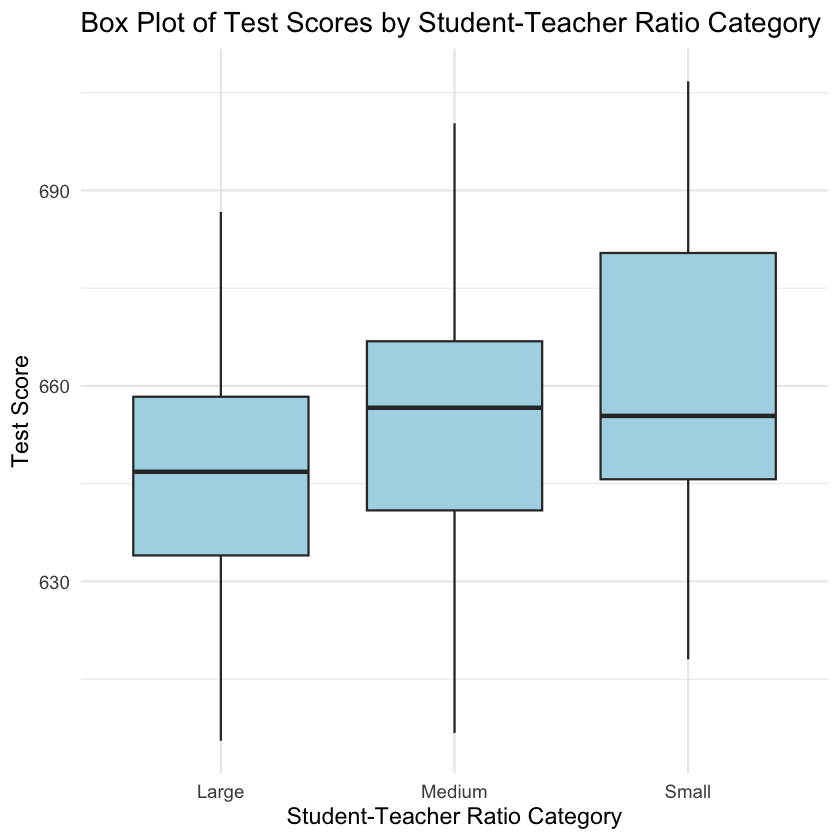
\includegraphics[width=4.375in,height=4.375in]{07_Lab-2_dummy-variable_files/figure-pdf/cell-14-output-1.png}

\subsection{Two-way ANOVA test}\label{two-way-anova-test}

The two-way ANOVA test is used to compare the fits of two regression
models.

\begin{itemize}
\item
  Test for Improvement: It tests whether adding more predictors
  (variables) to a model significantly improves the model's ability to
  explain the variability in the response variable.
\item
  Model Selection: Helps in deciding between a simpler model with fewer
  variables and a more complex one with more variables.
\end{itemize}

For instance, consider we have two models:

\begin{itemize}
\tightlist
\item
  Model 1: \(y = \beta_0 + \beta_1 x_{1} + \varepsilon\), and
\item
  Model 2:
  \(y = \beta_0 + \beta_1 x_{1} + \beta_2 x_2 + \beta_3 x_3 + \varepsilon\).
\end{itemize}

We can form a test by comparing the \(R^2\) from the two models.

\[
\begin{aligned}
&\text{H}_0: \beta_2 = \beta_3 = 0 \\
&\text{H}_1: \beta_2 \ne 0 \text{ or } \beta_3\ne 0 ,
\end{aligned}
\] which imposes two exclusion restrictions.

Coming back to our California school TestScore example, we can use the
two-way ANOVA test to see if the multiple regression model with
additional control variables (Model 2) significantly improves the
model's ability to explain the variability in TestScore compared to the
simple regression model (Model 1).

\begin{Shaded}
\begin{Highlighting}[]
\NormalTok{anova\_result2 }\OtherTok{\textless{}{-}} \FunctionTok{anova}\NormalTok{(dummy\_model\_slr, dummy\_model\_mlr)}
\NormalTok{anova\_result2}
\end{Highlighting}
\end{Shaded}

A anova: 2 × 6

\begin{longtable}[]{@{}
  >{\raggedright\arraybackslash}p{(\linewidth - 12\tabcolsep) * \real{0.1429}}
  >{\raggedright\arraybackslash}p{(\linewidth - 12\tabcolsep) * \real{0.1429}}
  >{\raggedright\arraybackslash}p{(\linewidth - 12\tabcolsep) * \real{0.1429}}
  >{\raggedright\arraybackslash}p{(\linewidth - 12\tabcolsep) * \real{0.1429}}
  >{\raggedright\arraybackslash}p{(\linewidth - 12\tabcolsep) * \real{0.1429}}
  >{\raggedright\arraybackslash}p{(\linewidth - 12\tabcolsep) * \real{0.1429}}
  >{\raggedright\arraybackslash}p{(\linewidth - 12\tabcolsep) * \real{0.1429}}@{}}
\toprule\noalign{}
\begin{minipage}[b]{\linewidth}\raggedright
\end{minipage} & \begin{minipage}[b]{\linewidth}\raggedright
Res.Df \textless dbl\textgreater{}
\end{minipage} & \begin{minipage}[b]{\linewidth}\raggedright
RSS \textless dbl\textgreater{}
\end{minipage} & \begin{minipage}[b]{\linewidth}\raggedright
Df \textless dbl\textgreater{}
\end{minipage} & \begin{minipage}[b]{\linewidth}\raggedright
Sum of Sq \textless dbl\textgreater{}
\end{minipage} & \begin{minipage}[b]{\linewidth}\raggedright
F \textless dbl\textgreater{}
\end{minipage} & \begin{minipage}[b]{\linewidth}\raggedright
Pr(\textgreater F) \textless dbl\textgreater{}
\end{minipage} \\
\midrule\noalign{}
\endhead
\bottomrule\noalign{}
\endlastfoot
1 & 418 & 146815.42 & NA & NA & NA & NA \\
2 & 415 & 34940.45 & 3 & 111875 & 442.9261 & 6.146085e-129 \\
\end{longtable}

The p-value is way less than 0.05, indicating that we reject the null
hypothesis and conclude that adding the control variables
(\texttt{computer}, \texttt{english}, and \texttt{lunch}) significantly
improves the model's ability to explain the variability in TestScore.

\chapter{Interactions of Binary
Variables}\label{interactions-of-binary-variables}

\begin{tcolorbox}[enhanced jigsaw, colframe=quarto-callout-note-color-frame, colback=white, opacityback=0, breakable, toprule=.15mm, arc=.35mm, leftrule=.75mm, rightrule=.15mm, left=2mm, bottomrule=.15mm]


\includegraphics[width=\linewidth,height=1em,keepaspectratio]{filters/emoji/1f3af.png}
\textbf{Study Objectives}

\begin{itemize}
\tightlist
\item
  Interpret interaction terms of two binary variables in regression
  models.
\item
  Understand the importance of controlling for changes in interacting
  variables when interpreting coefficients.
\item
  Conduct and interpret a two-way ANOVA to compare nested regression
  models.
\item
  Interpret interaction terms between a binary variable and a continuous
  variable in regression models.
\item
  Visualize interaction effects using regression lines.
\end{itemize}

\end{tcolorbox}

For this section of the course, we will be working with the
\texttt{Boston} dataset, which contains 506 observations on housing
values in various suburbs of Boston. This dataset provides detailed
information on factors such as crime rates, property age, locations
(proximity to the Charles River), and other socioeconomic variables.

We will use this data to \textbf{explore and analyze the determinants of
housing prices}, applying regression techniques to understand how
different factors influence the value of homes.

\begin{Shaded}
\begin{Highlighting}[]
\CommentTok{\# load packages and dataset}
\NormalTok{pkgs }\OtherTok{\textless{}{-}} \FunctionTok{c}\NormalTok{(}\StringTok{"tidyverse"}\NormalTok{, }\StringTok{"MASS"}\NormalTok{, }\StringTok{"data.table"}\NormalTok{, }\StringTok{"stargazer"}\NormalTok{, }\StringTok{"cowplot"}\NormalTok{)}
\NormalTok{missing }\OtherTok{\textless{}{-}} \FunctionTok{setdiff}\NormalTok{(pkgs, }\FunctionTok{rownames}\NormalTok{(}\FunctionTok{installed.packages}\NormalTok{()))}
\ControlFlowTok{if}\NormalTok{ (}\FunctionTok{length}\NormalTok{(missing) }\SpecialCharTok{\textgreater{}} \DecValTok{0}\NormalTok{) }\FunctionTok{install.packages}\NormalTok{(missing)}
\FunctionTok{invisible}\NormalTok{(}\FunctionTok{lapply}\NormalTok{(pkgs, }\ControlFlowTok{function}\NormalTok{(pkg) }\FunctionTok{suppressPackageStartupMessages}\NormalTok{(}\FunctionTok{library}\NormalTok{(pkg, }\AttributeTok{character.only =} \ConstantTok{TRUE}\NormalTok{))))}
\FunctionTok{data}\NormalTok{(Boston) }\CommentTok{\# Boston housing data}
\end{Highlighting}
\end{Shaded}

Use \texttt{?Boston} to see the description of the dataset.

Here are some variables in the dataset which we are going to use in this
session.

\begin{longtable}[]{@{}
  >{\raggedright\arraybackslash}p{(\linewidth - 2\tabcolsep) * \real{0.1304}}
  >{\raggedright\arraybackslash}p{(\linewidth - 2\tabcolsep) * \real{0.8696}}@{}}
\toprule\noalign{}
\begin{minipage}[b]{\linewidth}\raggedright
Variables
\end{minipage} & \begin{minipage}[b]{\linewidth}\raggedright
Definitions
\end{minipage} \\
\midrule\noalign{}
\endhead
\bottomrule\noalign{}
\endlastfoot
\texttt{medv} & median value of owner-occupied homes in \$1000s. \\
\texttt{lstat} & the percentage of individuals with low socioeconomic
status \\
\texttt{indus} & proportion of non-retail business acres per town;
industrial, office, or commercial land not directly serving
consumers. \\
\texttt{age} & proportion of owner-occupied units built prior to
1940. \\
\texttt{crim} & per capita crime rate by town. \\
\texttt{chas} & A dummy variable. Takes the value 1 if the Charles River
(a short river in the proximity of Boston) passes through the suburb and
is 0 otherwise. \\
\end{longtable}

\section{Interactions of Two Binary
Variables}\label{interactions-of-two-binary-variables}

Consider the following regression model

\begin{equation}\phantomsection\label{eq-binary-interaction}{
medv_i = \beta_0 + \beta_1\, chas_i + \beta_2\, old_i + \beta_3\, (chas_i \times old_i) + u_i
}\end{equation}

where \(chas_i\) and \(old_i\) are dummy variables defined as follows:

\[
\begin{aligned}
chas_i &= \begin{cases}
1 & \text{if the suburb is next to the Charles River} \\
0 & \text{otherwise}
\end{cases} \\
old_i &= \begin{cases}
1 & \text{if } age_i \ge 95 \\
0 & \text{otherwise}
\end{cases}
\end{aligned}
\]

where \(agi_i\) being the proportion of owner-occupied units built prior
to 1940.

\textbf{Instructions:}

\begin{itemize}
\tightlist
\item
  Generate and append the binary variable \(old\) to the dataset Boston.
\item
  Conduct the regression stated above and assign the result to
  \texttt{mod\_bb}.
\item
  Obtain a robust coefficient summary of the model. How do you interpret
  the results?
\end{itemize}

\begin{Shaded}
\begin{Highlighting}[]
\NormalTok{Boston }\OtherTok{\textless{}{-}}\NormalTok{ Boston }\SpecialCharTok{\%\textgreater{}\%}
    \FunctionTok{mutate}\NormalTok{(}\AttributeTok{old =} \FunctionTok{ifelse}\NormalTok{(age }\SpecialCharTok{\textgreater{}=} \DecValTok{95}\NormalTok{, }\DecValTok{1}\NormalTok{, }\DecValTok{0}\NormalTok{))}
\NormalTok{mod\_bb }\OtherTok{\textless{}{-}} \FunctionTok{lm}\NormalTok{(medv }\SpecialCharTok{\textasciitilde{}}\NormalTok{ chas}\SpecialCharTok{*}\NormalTok{old, }\AttributeTok{data =}\NormalTok{ Boston)}
\FunctionTok{summary}\NormalTok{(mod\_bb)}
\end{Highlighting}
\end{Shaded}

\begin{verbatim}

Call:
lm(formula = medv ~ chas * old, data = Boston)

Residuals:
    Min      1Q  Median      3Q     Max 
-17.771  -4.765  -1.683   2.776  33.433 

Coefficients:
            Estimate Std. Error t value Pr(>|t|)    
(Intercept)  23.6989     0.4503  52.624  < 2e-16 ***
chas          4.0582     1.6872   2.405   0.0165 *  
old          -7.1319     0.9493  -7.513 2.67e-13 ***
chas:old     10.5462     3.7577   2.807   0.0052 ** 
---
Signif. codes:  0 '***' 0.001 '**' 0.01 '*' 0.05 '.' 0.1 ' ' 1

Residual standard error: 8.604 on 502 degrees of freedom
Multiple R-squared:  0.1301,    Adjusted R-squared:  0.1249 
F-statistic: 25.02 on 3 and 502 DF,  p-value: 4.244e-15
\end{verbatim}

The estimated regression model is given by

\[
\widehat{medv}_i = 23.70 + 4.06\, chas_i - 7.13\, old_i + 10.55\, (chas_i \times old_i)
\]

{\textbf{Interpretation of the coefficients}}

We start with listing all possible combinations of the binary variables
\(chas_i\) and \(old_i\).

\begin{longtable}[]{@{}
  >{\raggedright\arraybackslash}p{(\linewidth - 6\tabcolsep) * \real{0.0435}}
  >{\raggedright\arraybackslash}p{(\linewidth - 6\tabcolsep) * \real{0.1159}}
  >{\raggedright\arraybackslash}p{(\linewidth - 6\tabcolsep) * \real{0.1014}}
  >{\raggedright\arraybackslash}p{(\linewidth - 6\tabcolsep) * \real{0.7391}}@{}}
\toprule\noalign{}
\begin{minipage}[b]{\linewidth}\raggedright
Scenario
\end{minipage} & \begin{minipage}[b]{\linewidth}\raggedright
\(chas_i\)
\end{minipage} & \begin{minipage}[b]{\linewidth}\raggedright
\(old_i\)
\end{minipage} & \begin{minipage}[b]{\linewidth}\raggedright
Interpretation
\end{minipage} \\
\midrule\noalign{}
\endhead
\bottomrule\noalign{}
\endlastfoot
\textbf{1} & 0 & 0 & Suburb not next to Charles River and new \\
\textbf{2} & 0 & 1 & Suburb not next to Charles River and old \\
\textbf{3} & 1 & 0 & Suburb next to Charles River and new \\
\textbf{4} & 1 & 1 & Suburb next to Charles River and old \\
\end{longtable}

Based on the estimated regression model, we can compute the expected
value of \texttt{medv} for each of the four groups.

\begin{longtable}[]{@{}
  >{\centering\arraybackslash}p{(\linewidth - 8\tabcolsep) * \real{0.0704}}
  >{\centering\arraybackslash}p{(\linewidth - 8\tabcolsep) * \real{0.0704}}
  >{\centering\arraybackslash}p{(\linewidth - 8\tabcolsep) * \real{0.0634}}
  >{\centering\arraybackslash}p{(\linewidth - 8\tabcolsep) * \real{0.1620}}
  >{\raggedright\arraybackslash}p{(\linewidth - 8\tabcolsep) * \real{0.6338}}@{}}
\toprule\noalign{}
\begin{minipage}[b]{\linewidth}\centering
Scenario
\end{minipage} & \begin{minipage}[b]{\linewidth}\centering
\(chas_i\)
\end{minipage} & \begin{minipage}[b]{\linewidth}\centering
\(old_i\)
\end{minipage} & \begin{minipage}[b]{\linewidth}\centering
\(chas_i \times old_i\)
\end{minipage} & \begin{minipage}[b]{\linewidth}\raggedright
Expected value of \texttt{medv}
\end{minipage} \\
\midrule\noalign{}
\endhead
\bottomrule\noalign{}
\endlastfoot
\textbf{1} & 0 & 0 & 0 &
\(\color[HTML]{0099FF}{\hat{\beta}_0} = 23.70\) \\
\textbf{2} & 0 & 1 & 0 &
\({\color[HTML]{0099FF}\hat{\beta}_0} + {\color[HTML]{00CC66}\hat{\beta}_2} = {\color[HTML]{0099FF}23.70} + {\color[HTML]{00CC66}(- 7.13)} = 16.57\) \\
\textbf{3} & 1 & 0 & 0 &
\({\color[HTML]{0099FF}\hat{\beta}_0} + {\color[HTML]{fb5b89}\hat{\beta}_1} = {\color[HTML]{0099FF}23.70} + {\color[HTML]{fb5b89}4.06} = 27.76\) \\
\textbf{4} & 1 & 1 & 1 &
\({\color[HTML]{0099FF}\hat{\beta}_0} + {\color[HTML]{fb5b89}\hat{\beta}_1} + {\color[HTML]{00CC66}\hat{\beta}_2} + {\color{orange}\hat{\beta}_3} = {\color[HTML]{0099FF}23.70} + {\color[HTML]{fb5b89}4.06} + {\color[HTML]{00CC66}(-7.13)} + {\color{orange}(10.55)} = 31.18\) \\
\end{longtable}

From the table above, we can interpret the coefficients as follows:

\begin{itemize}
\item
  \(\color[HTML]{0099FF}{\hat{\beta}_0} = 23.70\) is the expected value
  of \texttt{medv} for suburbs that are not next to the Charles River
  and are new (i.e., \texttt{old\ =\ 0}).
\item
  Comparing scenario 2 with 1:
  \(\color[HTML]{00CC66}{\hat{\beta}_2} = -7.13\) is the difference in
  expected value of \texttt{medv} between new and old suburbs that are
  \textbf{NOT next to the Charles River}.

  In other words, old suburbs that are not next to the Charles River
  have an expected \texttt{medv} that is 7.13 lower than new suburbs
  that are \textbf{NOT next to the Charles River}.
\item
  Comparing scenario 3 with 1:
  \(\color[HTML]{fb5b89}{\hat{\beta}_1} = 4.06\) is the difference in
  expected value of \texttt{medv} between suburbs that are next to the
  Charles River and those that are not, among \textbf{new} suburbs
  (i.e., \texttt{old\ =\ 0}).

  In other words, \textbf{new} suburbs that are next to the Charles
  River have an expected \texttt{medv} that is 4.06 higher than new
  suburbs that are not next to the Charles River.
\item
  \(\color{orange}{\hat{\beta}_3} = 10.55\) has two interpretations:

  \begin{itemize}
  \item
    If we compare scenario 4 with scenario 2, the difference in expected
    value of \texttt{medv} is given by
    \({\color[HTML]{fb5b89}\hat{\beta}_1} + {\color{orange}\hat{\beta}_3} = 4.06 + 10.55 = 14.61.\)

    This means that \textbf{old} suburbs that are next to the Charles
    River have an expected \texttt{medv} that is 14.61 higher than
    \textbf{old} suburbs that are not next to the Charles River.

    → \(\color{orange}{\hat{\beta}_3}\) can be interpreted as the
    difference in the effect of being next to the Charles River between
    old and new suburbs.
  \item
    If we compare scenario 4 with scenario 3, the difference in expected
    value of \texttt{medv} is given by
    \({\color[HTML]{00CC66}\hat{\beta}_2} + {\color{orange}\hat{\beta}_3} = -7.13 + 10.55 = 3.42.\)

    This means that old suburbs that are \textbf{next to the Charles
    River} have an expected \texttt{medv} that is 3.42 higher than new
    suburbs that are \textbf{next to the Charles River}.

    → \(\color{orange}{\hat{\beta}_3}\) can be interpreted as the
    difference in the effect of being old between suburbs that are next
    to the Charles River and those that are not.
  \end{itemize}
\end{itemize}

\begin{tcolorbox}[enhanced jigsaw, colframe=quarto-callout-tip-color-frame, colback=white, opacityback=0, breakable, coltitle=black, opacitybacktitle=0.6, toptitle=1mm, colbacktitle=quarto-callout-tip-color!10!white, arc=.35mm, bottomtitle=1mm, titlerule=0mm, toprule=.15mm, title=\textcolor{quarto-callout-tip-color}{\faLightbulb}\hspace{0.5em}{Tip}, leftrule=.75mm, rightrule=.15mm, left=2mm, bottomrule=.15mm]

{\textbf{Controlling for changes in the interacting variables}} is
essential when interpreting the coefficient of interaction terms.

A common approach is to substitute specific values for the interacting
variables and compute the expected value of the dependent variable under
different scenarios. This allows for a clearer interpretation of the
coefficients by comparing how the expected value of the dependent
variable varies across these scenarios.

\end{tcolorbox}

\subsection{Add More Controls
Variables}\label{add-more-controls-variables}

We can also add more control variables to
Equation~\ref{eq-binary-interaction} to improve the model fit (Adjusted
\(R^2 = 12\%\) as of now). For example, we can add \texttt{lstat} and
\texttt{crim} as additional control variables.

\begin{equation}\phantomsection\label{eq-binary-interaction-more-controls}{
medv_i = \beta_0 + \beta_1\, chas_i + \beta_2\, old_i + \beta_3\, (chas_i \times old_i) + \beta_4\, lstat_i + \beta_5\, crim_i + u_i
}\end{equation}

We estimate the above regression model as follows.

\begin{Shaded}
\begin{Highlighting}[]
\NormalTok{mod\_bb2 }\OtherTok{\textless{}{-}} \FunctionTok{lm}\NormalTok{(medv }\SpecialCharTok{\textasciitilde{}}\NormalTok{ chas }\SpecialCharTok{*}\NormalTok{ old }\SpecialCharTok{+}\NormalTok{ lstat }\SpecialCharTok{+}\NormalTok{ crim, }\AttributeTok{data =}\NormalTok{ Boston)}
\CommentTok{\# reorder the variables for stargazer output}
\NormalTok{vars.order }\OtherTok{\textless{}{-}} \FunctionTok{c}\NormalTok{(}\StringTok{"chas"}\NormalTok{, }\StringTok{"old"}\NormalTok{, }\StringTok{"chas:old"}\NormalTok{, }\StringTok{"lstat"}\NormalTok{, }\StringTok{"crim"}\NormalTok{)}
\FunctionTok{stargazer}\NormalTok{(mod\_bb, mod\_bb2,}
    \AttributeTok{type =} \StringTok{"text"}\NormalTok{,}
    \AttributeTok{column.labels =} \FunctionTok{c}\NormalTok{(}\StringTok{"Restricted"}\NormalTok{, }\StringTok{"Unrestricted"}\NormalTok{),}
    \AttributeTok{order =} \FunctionTok{paste0}\NormalTok{(}\StringTok{"\^{}"}\NormalTok{, vars.order, }\StringTok{"$"}\NormalTok{)}
\NormalTok{)}
\end{Highlighting}
\end{Shaded}

\begin{verbatim}

====================================================================
                                  Dependent variable:               
                    ------------------------------------------------
                                          medv                      
                          Restricted              Unrestricted      
                              (1)                     (2)           
--------------------------------------------------------------------
chas                        4.058**                 4.000***        
                            (1.687)                 (1.183)         
                                                                    
old                        -7.132***                1.748**         
                            (0.949)                 (0.776)         
                                                                    
chas:old                   10.546***                 4.008          
                            (3.758)                 (2.651)         
                                                                    
lstat                                              -0.949***        
                                                    (0.046)         
                                                                    
crim                                                -0.079**        
                                                    (0.036)         
                                                                    
Constant                   23.699***               34.106***        
                            (0.450)                 (0.573)         
                                                                    
--------------------------------------------------------------------
Observations                  506                     506           
R2                           0.130                   0.574          
Adjusted R2                  0.125                   0.570          
Residual Std. Error    8.604 (df = 502)         6.033 (df = 500)    
F Statistic         25.017*** (df = 3; 502) 134.705*** (df = 5; 500)
====================================================================
Note:                                    *p<0.1; **p<0.05; ***p<0.01
\end{verbatim}

\textbf{Comparing the two models:}

\begin{itemize}
\tightlist
\item
  The coefficient of \texttt{old} reversed signs, from negative
  (\(-7.13\)) to positive (\(1.75\)), suggesting that after accounting
  for crime and low socioeconomic status, older suburbs have slightly
  higher values.
\item
  Negative coefficients for \texttt{lstat} (\(-0.95\)) and \texttt{crim}
  (\(-0.079\)) indicate that higher poverty and crime reduce house
  values.
\end{itemize}

Plot \texttt{lstat} and \texttt{crim} group by \texttt{old} to see how
the distribution of these two variables differ between new and old
suburbs.

\begin{Shaded}
\begin{Highlighting}[]
\NormalTok{p1 }\OtherTok{\textless{}{-}} \FunctionTok{ggplot}\NormalTok{(Boston, }\FunctionTok{aes}\NormalTok{(}\AttributeTok{x =} \FunctionTok{factor}\NormalTok{(old), }\AttributeTok{y =}\NormalTok{ lstat)) }\SpecialCharTok{+}
    \FunctionTok{geom\_boxplot}\NormalTok{(}\AttributeTok{fill =} \StringTok{"lightblue"}\NormalTok{)}
\NormalTok{p2 }\OtherTok{\textless{}{-}} \FunctionTok{ggplot}\NormalTok{(Boston, }\FunctionTok{aes}\NormalTok{(}\AttributeTok{x =} \FunctionTok{factor}\NormalTok{(old), }\AttributeTok{y =}\NormalTok{ crim)) }\SpecialCharTok{+}
    \FunctionTok{geom\_boxplot}\NormalTok{(}\AttributeTok{fill =} \StringTok{"lightblue"}\NormalTok{)}
\FunctionTok{plot\_grid}\NormalTok{(p1, p2, }\AttributeTok{labels =} \FunctionTok{c}\NormalTok{(}\StringTok{"A"}\NormalTok{, }\StringTok{"B"}\NormalTok{), }\AttributeTok{ncol =} \DecValTok{2}\NormalTok{)}
\end{Highlighting}
\end{Shaded}

\pandocbounded{
\includegraphics[keepaspectratio]{08_Interactions_files/figure-pdf/unnamed-chunk-4-1.pdf}}

We see that old suburbs tend to have higher \texttt{lstat} and
\texttt{crim} values compared to new suburbs. This suggests that
controlling for these variables is important when examining the
relationship between \texttt{medv}, \texttt{chas}, and \texttt{old}.

\subsection{Two-Way ANOVA Mathematical
Formulation}\label{two-way-anova-mathematical-formulation}

We now conduct a two-way ANOVA to formally compare the two models
\texttt{mod\_bb} and \texttt{mod\_bb2}.

\begin{Shaded}
\begin{Highlighting}[]
\FunctionTok{anova}\NormalTok{(mod\_bb, mod\_bb2)}
\end{Highlighting}
\end{Shaded}

\begin{verbatim}
Analysis of Variance Table

Model 1: medv ~ chas * old
Model 2: medv ~ chas * old + lstat + crim
  Res.Df   RSS Df Sum of Sq      F    Pr(>F)    
1    502 37161                                  
2    500 18200  2     18961 260.45 < 2.2e-16 ***
---
Signif. codes:  0 '***' 0.001 '**' 0.01 '*' 0.05 '.' 0.1 ' ' 1
\end{verbatim}

\begin{enumerate}
\def\labelenumi{\arabic{enumi}.}
\item
  State the null and alternative hypotheses. \[
  \begin{aligned}
  H_0 &: \beta_4 = 0 \text{ and } \beta_5 = 0 \\
  H_1 &: \beta_4 \ne 0 \text{ or } \beta_5 \ne 0
  \end{aligned}
  \]

  In plain language:

  \begin{itemize}
  \tightlist
  \item
    \(H_0\): The additional variables \texttt{lstat} and \texttt{crim}
    do not improve the model fit.
  \item
    \(H_1\): At least one of the additional variables \texttt{lstat} or
    \texttt{crim} improves the model fit.
  \end{itemize}
\item
  Calculate the F-statistic.

  The F-statistic is based on the \(R^2\) of the two regressions: \[
  F = \left(\frac{n - k_U -1}{p}\right) \left(\frac{R_U^2-R_R^2}{1-R_U^2}\right) \sim F(p, n-k_U-1) .
  \]

  where

  \begin{itemize}
  \tightlist
  \item
    \(n = 506\) is the number of observations;
  \item
    \(k_U = 5\) is the number of predictors in the unrestricted model
    (where \(H_1\) is allowed to be true), excluding the intercept;
  \item
    \(p = 2\) is the number of restrictions (i.e., the number of
    additional variables in the unrestricted model);
  \item
    \(R_U^2 = 0.574\) is the \(R^2\) of the unrestricted model;
  \item
    \(R_R^2 = 0.130\) is the \(R^2\) of the restricted model.
  \end{itemize}

  Plug in the numbers, we get \[
  F = \left(\frac{506-5-1}{2}\right) \left(\frac{0.574-0.130}{1-0.574}\right) = 260.56
  \]
\item
  Find the critical value

  The F-statistic follows an \(F(2, 502)\) distribution under the null
  hypothesis. At 5\% significance level, we use the the critical value
  \(F_{2,\infty}=3.00.\)
\item
  Decision rule.

  Since the calculated F-statistic (\(260.56\)) is much larger than the
  critical value (\(3.00\)), we reject the null hypothesis.

  This suggests that at least one of \texttt{lstat} and \texttt{crim}
  significantly improves the model fit.
\item
  Conclusion.

  We conclude that model (2) with additional control variables
  \texttt{lstat} and \texttt{crim} provides a significantly better fit
  to the data compared to model (1) without these controls.
\end{enumerate}

\section{Interactions of a Binary Variable and a Continuous
Variable}\label{interactions-of-a-binary-variable-and-a-continuous-variable}

An interaction between a binary variable and a continuous variable shows
how the effect of the continuous variable changes depending on the
group. This helps us see differences that a simple line wouldn't
capture. For example, the effect of business area on house prices might
be different in new versus old suburbs.

Now consider the regression model

\[
medv_i = \beta_0 + \beta_1 \times indus_i + \beta_2 \times old_i + \beta_3 \times (indus_i\times old_i) + u_i
\]

where \(indus_i\) being the proportion of non-retail business acres in
suburb \(i\); \(old_i\) is the same binary variable as defined above,
indicating if the suburb is new.

\textbf{Instructions:}

\begin{itemize}
\tightlist
\item
  Estimate the above regression model and assign the result to
  \texttt{mod\_bc}.
\item
  What is the relationship between \texttt{medv} and \texttt{indus} for
  new suburbs? What about old suburbs?
\item
  Is the effect of \texttt{indus} on \texttt{medv} statistically
  different between new and old suburbs?
\item
  Plot \texttt{medv} against \texttt{indus} and add the regression lines
  for both states of the binary variable \texttt{old}.
\end{itemize}

\begin{Shaded}
\begin{Highlighting}[]
\NormalTok{mod\_bc }\OtherTok{\textless{}{-}} \FunctionTok{lm}\NormalTok{(medv }\SpecialCharTok{\textasciitilde{}}\NormalTok{ indus }\SpecialCharTok{*}\NormalTok{ old, }\AttributeTok{data =}\NormalTok{ Boston)}
\FunctionTok{summary}\NormalTok{(mod\_bc)}
\end{Highlighting}
\end{Shaded}

\begin{verbatim}

Call:
lm(formula = medv ~ indus * old, data = Boston)

Residuals:
    Min      1Q  Median      3Q     Max 
-12.379  -5.066  -1.588   3.015  33.046 

Coefficients:
            Estimate Std. Error t value Pr(>|t|)    
(Intercept) 30.06350    0.72882  41.250   <2e-16 ***
indus       -0.65844    0.06569 -10.024   <2e-16 ***
old         -7.48438    3.07918  -2.431   0.0154 *  
indus:old    0.37115    0.17558   2.114   0.0350 *  
---
Signif. codes:  0 '***' 0.001 '**' 0.01 '*' 0.05 '.' 0.1 ' ' 1

Residual standard error: 8.024 on 502 degrees of freedom
Multiple R-squared:  0.2434,    Adjusted R-squared:  0.2389 
F-statistic: 53.83 on 3 and 502 DF,  p-value: < 2.2e-16
\end{verbatim}

The estimated regression model is given by

\[
\widehat{medv}_i = 30.06 - 0.66 \times indus_i - 7.48 \times old_i + 0.37 \times (indus_i \cdot old_i)
\]

{\textbf{Interpretation of the coefficients}}

\begin{itemize}
\item
  For new suburbs (i.e., \texttt{old\ =\ 0}), the relationship between
  \texttt{medv} and \texttt{indus} is given by

  \[
  E(medv_i | old_i = 0) = \hat{\beta}_0 + \hat{\beta}_1 \times indus_i = 30.06 - 0.66 \times indus_i
  \]

  Thus, for new suburbs, a one-unit increase in \texttt{indus} is
  associated with a decrease in the expected value of \texttt{medv} by
  0.66.
\item
  For old suburbs (i.e., \texttt{old\ =\ 1}), the relationship between
  \texttt{medv} and \texttt{indus} is given by

  \[
  \begin{split}
  E(medv_i | old_i = 1) &= (\hat{\beta}_0 + \hat{\beta}_2) + (\hat{\beta}_1 + \hat{\beta}_3) \times indus_i \\
  &= (30.06 - 7.48) + (-0.66 + 0.37) \times indus_i \\
  &= 22.58 - 0.29 \times indus_i
  \end{split}
  \]

  Thus, for old suburbs, a one-unit increase in \texttt{indus} is
  associated with a decrease in the expected value of \texttt{medv} by
  0.29. The negative effect is smaller in old suburbs due to the
  positive interaction term (\(\hat{\beta}_3 = 0.37\)).
\item
  The effect of \texttt{indus} on \texttt{medv} is statistically
  different between new and old suburbs at 5\% significance level given
  that the coefficient of the interaction term (\(\hat{\beta}_3\)) is
  statistically significant.
\end{itemize}

\textbf{Visualization}

Now we plot \texttt{medv} against \texttt{indus} with regression lines
for both states of the binary variable \texttt{old}.

\begin{Shaded}
\begin{Highlighting}[]
\FunctionTok{ggplot}\NormalTok{(Boston, }\FunctionTok{aes}\NormalTok{(}\AttributeTok{x =}\NormalTok{ indus, }\AttributeTok{y =}\NormalTok{ medv, }\AttributeTok{color =} \FunctionTok{factor}\NormalTok{(old))) }\SpecialCharTok{+}
    \FunctionTok{geom\_point}\NormalTok{(}\AttributeTok{alpha =} \FloatTok{0.6}\NormalTok{) }\SpecialCharTok{+}
    \FunctionTok{geom\_smooth}\NormalTok{(}\AttributeTok{method =} \StringTok{"lm"}\NormalTok{, }\AttributeTok{formula =}\NormalTok{ y }\SpecialCharTok{\textasciitilde{}}\NormalTok{ x, }\AttributeTok{se =} \ConstantTok{FALSE}\NormalTok{) }\SpecialCharTok{+}
    \FunctionTok{labs}\NormalTok{(}
        \AttributeTok{x =} \StringTok{"Proportion of Non{-}Retail Business Acres (indus)"}\NormalTok{,}
        \AttributeTok{y =} \StringTok{"Median Home Value (medv)"}\NormalTok{,}
        \AttributeTok{color =} \StringTok{"Old Suburb (old)"}
\NormalTok{    ) }\SpecialCharTok{+}
    \FunctionTok{scale\_color\_manual}\NormalTok{(}\AttributeTok{values =} \FunctionTok{c}\NormalTok{(}\StringTok{"0"} \OtherTok{=} \StringTok{"blue"}\NormalTok{, }\StringTok{"1"} \OtherTok{=} \StringTok{"red"}\NormalTok{), }\AttributeTok{labels =} \FunctionTok{c}\NormalTok{(}\StringTok{"New Suburb"}\NormalTok{, }\StringTok{"Old Suburb"}\NormalTok{)) }\SpecialCharTok{+}
    \FunctionTok{theme\_minimal}\NormalTok{(}\AttributeTok{base\_size =} \DecValTok{14}\NormalTok{) }\SpecialCharTok{+}
    \FunctionTok{theme}\NormalTok{(}
        \AttributeTok{legend.title =} \FunctionTok{element\_blank}\NormalTok{(),}
        \AttributeTok{legend.text =} \FunctionTok{element\_text}\NormalTok{(}\AttributeTok{size =} \DecValTok{14}\NormalTok{),}
        \AttributeTok{legend.position =} \FunctionTok{c}\NormalTok{(}\FloatTok{0.8}\NormalTok{, }\FloatTok{0.9}\NormalTok{)}
\NormalTok{    )}
\end{Highlighting}
\end{Shaded}

\pandocbounded{
\includegraphics[keepaspectratio]{08_Interactions_files/figure-pdf/unnamed-chunk-7-1.pdf}}

We see that the slope of the regression line for new suburbs (blue) is
steeper than that for old suburbs (red), indicating a stronger negative
relationship between \texttt{medv} and \texttt{indus} in new suburbs
compared to old suburbs. This visual representation aligns with our
earlier interpretation of the regression coefficients.

\chapter{Regression with a Binary Dependent
Variable}\label{regression-with-a-binary-dependent-variable}

\begin{tcolorbox}[enhanced jigsaw, colframe=quarto-callout-note-color-frame, colback=white, opacityback=0, breakable, toprule=.15mm, arc=.35mm, leftrule=.75mm, rightrule=.15mm, left=2mm, bottomrule=.15mm]


\includegraphics[width=\linewidth,height=1em,keepaspectratio]{filters/emoji/1f3af.png}
\textbf{Study Objectives}

\begin{itemize}
\tightlist
\item
  Understand why linear regression is inappropriate for binary dependent
  variables.
\item
  Learn the logit and probit models for analyzing binary outcomes.
\item
  Interpret coefficients in logistic regressions.
\item
  Apply logit/probit models using real-world data (HMDA mortgage
  application dataset).
\item
  Understand the concept of predicted probabilities.
\item
  Compare linear probability model (LPM), logit, and probit approaches.
\end{itemize}

\end{tcolorbox}

\section{Why Binary Dependent Variables Require Special
Treatment}\label{why-binary-dependent-variables-require-special-treatment}

In many economic and financial applications, the dependent variable is
\textbf{binary} (takes only two values: 0 or 1). Examples include:

\begin{itemize}
\tightlist
\item
  \textbf{Mortgage approval}: Did the bank approve the mortgage
  application? (Yes = 1, No = 0)
\item
  \textbf{Labor force participation}: Is the individual employed? (Yes =
  1, No = 0)
\item
  \textbf{Default risk}: Did the borrower default on the loan? (Yes = 1,
  No = 0)
\item
  \textbf{Market entry}: Does the firm enter the market? (Yes = 1, No =
  0)
\item
  \textbf{Product choice}: Does the consumer purchase the product? (Yes
  = 1, No = 0)
\end{itemize}

\subsection{Why Linear Regression
Fails}\label{why-linear-regression-fails}

If we try to use ordinary linear regression (OLS) with a binary
dependent variable \(Y_i \in \{0,1\}\):

\[
Y_i = \beta_0 + \beta_1 X_{1i} + \beta_2 X_{2i} + \cdots + \beta_k X_{ki} + u_i
\]

This approach is called the \textbf{Linear Probability Model (LPM)}
because it estimates the probability that \(Y_i = 1\) as a linear
function of the predictors.

\textbf{Problems with LPM:}

\begin{enumerate}
\def\labelenumi{\arabic{enumi}.}
\item
  \textbf{Predicted probabilities outside {[}0,1{]}}: OLS can produce
  fitted values \(\hat{Y}_i < 0\) or \(\hat{Y}_i > 1\), which makes no
  sense for probabilities.
\item
  \textbf{Heteroskedasticity}: The error term variance depends on \(X\),
  violating the homoskedasticity assumption. This means standard errors
  are incorrect.
\item
  \textbf{Nonlinear relationship}: The effect of \(X\) on the
  probability of \(Y=1\) is unlikely to be constant across all values of
  \(X\). For example, increasing income from \textbackslash\$20,000 to
  \textbackslash\$30,000 likely has a different effect on mortgage
  approval than increasing from \textbackslash\$200,000 to
  \textbackslash\$210,000.
\end{enumerate}

\subsection{The Solution: Logit and Probit
Models}\label{the-solution-logit-and-probit-models}

To address these problems, we use \textbf{nonlinear models} that ensure
predicted probabilities stay within {[}0,1{]}:

\begin{itemize}
\tightlist
\item
  \textbf{Logit model}: Uses the logistic cumulative distribution
  function (CDF)
\item
  \textbf{Probit model}: Uses the standard normal cumulative
  distribution function (CDF)
\end{itemize}

\section{The HMDA Dataset: Mortgage Lending
Discrimination}\label{the-hmda-dataset-mortgage-lending-discrimination}

We will use data from the \textbf{Federal Reserve Bank of Boston}
collected under the \textbf{Home Mortgage Disclosure Act (HMDA)}. The
dataset contains information on mortgage applications in the Boston area
in 1990. The dataset contains 2380 observations with 14 variables.

\textbf{Research Question:} Do banks discriminate against minority
applicants when making mortgage lending decisions, after controlling for
economic factors?

\subsection{Load the Data}\label{load-the-data}

\begin{Shaded}
\begin{Highlighting}[]
\CommentTok{\# Load required packages}
\NormalTok{pkgs }\OtherTok{\textless{}{-}} \FunctionTok{c}\NormalTok{(}\StringTok{"AER"}\NormalTok{, }\StringTok{"tidyverse"}\NormalTok{, }\StringTok{"stargazer"}\NormalTok{, }\StringTok{"margins"}\NormalTok{, }\StringTok{"data.table"}\NormalTok{)}
\NormalTok{missing }\OtherTok{\textless{}{-}} \FunctionTok{setdiff}\NormalTok{(pkgs, }\FunctionTok{rownames}\NormalTok{(}\FunctionTok{installed.packages}\NormalTok{()))}
\ControlFlowTok{if}\NormalTok{ (}\FunctionTok{length}\NormalTok{(missing) }\SpecialCharTok{\textgreater{}} \DecValTok{0}\NormalTok{) }\FunctionTok{install.packages}\NormalTok{(missing)}
\FunctionTok{invisible}\NormalTok{(}\FunctionTok{lapply}\NormalTok{(pkgs, }\ControlFlowTok{function}\NormalTok{(pkg) }\FunctionTok{suppressPackageStartupMessages}\NormalTok{(}\FunctionTok{library}\NormalTok{(pkg, }\AttributeTok{character.only =} \ConstantTok{TRUE}\NormalTok{))))}

\CommentTok{\# Load HMDA data}
\FunctionTok{data}\NormalTok{(}\StringTok{"HMDA"}\NormalTok{)}

\CommentTok{\# Preview the data}
\FunctionTok{data.table}\NormalTok{(HMDA)}
\end{Highlighting}
\end{Shaded}

\begin{verbatim}
        deny pirat hirat     lvrat  chist  mhist  phist unemp selfemp insurance
      <fctr> <num> <num>     <num> <fctr> <fctr> <fctr> <num>  <fctr>    <fctr>
   1:     no 0.221 0.221 0.8000000      5      2     no   3.9      no        no
   2:     no 0.265 0.265 0.9218750      2      2     no   3.2      no        no
   3:     no 0.372 0.248 0.9203980      1      2     no   3.2      no        no
   4:     no 0.320 0.250 0.8604651      1      2     no   4.3      no        no
   5:     no 0.360 0.350 0.6000000      1      1     no   3.2      no        no
  ---                                                                          
2376:     no 0.310 0.250 0.8000000      1      1     no   3.2     yes        no
2377:     no 0.300 0.300 0.7770492      1      2     no   3.2      no        no
2378:     no 0.260 0.200 0.5267606      2      1     no   3.1      no        no
2379:    yes 0.320 0.260 0.7538462      6      1    yes   3.1      no        no
2380:    yes 0.350 0.260 0.8135593      2      2     no   4.3      no        no
      condomin   afam single hschool
        <fctr> <fctr> <fctr>  <fctr>
   1:       no     no     no     yes
   2:       no     no    yes     yes
   3:       no     no     no     yes
   4:       no     no     no     yes
   5:       no     no     no     yes
  ---                               
2376:       no     no     no     yes
2377:      yes     no    yes     yes
2378:       no     no     no     yes
2379:      yes    yes    yes     yes
2380:      yes     no    yes     yes
\end{verbatim}

\subsection{Variable Definitions}\label{variable-definitions}

The key variables in the HMDA dataset are:

\begin{itemize}
\tightlist
\item
  We will mainly use \texttt{deny}, \texttt{pirat}, and \texttt{afam} in
  our analysis.
\end{itemize}

\begin{longtable}[]{@{}
  >{\raggedright\arraybackslash}p{(\linewidth - 2\tabcolsep) * \real{0.4545}}
  >{\raggedright\arraybackslash}p{(\linewidth - 2\tabcolsep) * \real{0.5455}}@{}}
\toprule\noalign{}
\begin{minipage}[b]{\linewidth}\raggedright
Variable
\end{minipage} & \begin{minipage}[b]{\linewidth}\raggedright
Definition
\end{minipage} \\
\midrule\noalign{}
\endhead
\bottomrule\noalign{}
\endlastfoot
{\texttt{deny}} & Was the mortgage application denied? (yes/no) ---
\textbf{dependent variable} \\
{\texttt{pirat}} & Payments-to-income ratio (monthly loan payments /
monthly income) \\
{\texttt{afam}} & Is the applicant African American? (yes/no) \\
\texttt{hirat} & Housing expense-to-income ratio (monthly housing
expenses / monthly income) \\
\texttt{lvrat} & Loan-to-value ratio (loan amount / assessed property
value) \\
\texttt{chist} & Credit history: consumer credit score \\
\texttt{mhist} & Mortgage history: mortgage credit score \\
\texttt{phist} & Public record history: coded as ``no'' or ``yes'' (any
bankruptcies, tax liens, etc.) \\
\texttt{insurance} & Was mortgage insurance denied? (yes/no) \\
\texttt{selfemp} & Is the applicant self-employed? (yes/no) \\
\texttt{single} & Is the applicant single? (yes/no) \\
\texttt{hschool} & Does the applicant have high school education?
(yes/no) \\
\texttt{unemp} & 1989 Massachusetts unemployment rate in applicant's
industry (\%). \\
\texttt{condominium} & Is the property a condominium? (yes/no) \\
\end{longtable}

\subsection{Data Exploration}\label{data-exploration}

\subsubsection{Frequency Tables and Contingency
Tables}\label{frequency-tables-and-contingency-tables}

\textbf{Let's examine the denial rates overall and by race.}

We first look at the overall denial counts and rates.

\begin{Shaded}
\begin{Highlighting}[]
\CommentTok{\# Overall denial counts}
\FunctionTok{cat}\NormalTok{(}\StringTok{"Overall Denial Counts:}\SpecialCharTok{\textbackslash{}n}\StringTok{"}\NormalTok{)}
\FunctionTok{with}\NormalTok{(HMDA, }\FunctionTok{table}\NormalTok{(deny))}

\CommentTok{\# Overall denial rate}
\FunctionTok{cat}\NormalTok{(}\StringTok{"===========================}\SpecialCharTok{\textbackslash{}n}\StringTok{"}\NormalTok{)}
\FunctionTok{cat}\NormalTok{(}\StringTok{"Overall Denial Rate:}\SpecialCharTok{\textbackslash{}n}\StringTok{"}\NormalTok{)}
\FunctionTok{with}\NormalTok{(HMDA, }\FunctionTok{prop.table}\NormalTok{(}\FunctionTok{table}\NormalTok{(deny))) }\SpecialCharTok{\%\textgreater{}\%} \FunctionTok{round}\NormalTok{(}\DecValTok{3}\NormalTok{)}
\end{Highlighting}
\end{Shaded}

\begin{verbatim}
Overall Denial Counts:
deny
  no  yes 
2095  285 
===========================
Overall Denial Rate:
deny
  no  yes 
0.88 0.12 
\end{verbatim}

The table shows that about 12\% of mortgage applications were denied
overall. The majority of applications (88\%) were approved.

Next, we examine denial counts and rates by race.

A {\textbf{contingency table}} is an effective method to see the
association between two categorical variables. It counts the number of
observations in each of the four possible scenarios. When dealing with
just one categorical variable, this is referred to as a
\textbf{frequency table}, which count the number of observations for
each category.

The following gives a 2x2 contingency table for mortgage denial by
African-American or not.

\begin{Shaded}
\begin{Highlighting}[]
\CommentTok{\# Denial rate by race}
\FunctionTok{cat}\NormalTok{(}\StringTok{"Denail counts by race:}\SpecialCharTok{\textbackslash{}n}\StringTok{"}\NormalTok{)}
\FunctionTok{with}\NormalTok{(HMDA, }\FunctionTok{table}\NormalTok{(deny, afam))}
\FunctionTok{cat}\NormalTok{(}\StringTok{"===========================}\SpecialCharTok{\textbackslash{}n}\StringTok{"}\NormalTok{)}
\FunctionTok{cat}\NormalTok{(}\StringTok{"Denial rate by race:}\SpecialCharTok{\textbackslash{}n}\StringTok{"}\NormalTok{)}
\FunctionTok{with}\NormalTok{(HMDA, }\FunctionTok{prop.table}\NormalTok{(}\FunctionTok{table}\NormalTok{(deny, afam), }\AttributeTok{margin =} \DecValTok{2}\NormalTok{)) }\SpecialCharTok{\%\textgreater{}\%} \FunctionTok{round}\NormalTok{(}\DecValTok{3}\NormalTok{)}
\end{Highlighting}
\end{Shaded}

\begin{verbatim}
Denail counts by race:
     afam
deny    no  yes
  no  1852  243
  yes  189   96
===========================
Denial rate by race:
     afam
deny     no   yes
  no  0.907 0.717
  yes 0.093 0.283
\end{verbatim}

Some observations from the table:

\begin{itemize}
\tightlist
\item
  The majority of applicants are non-African American.
\item
  African American applicants have a higher denial rate (about 28\%)
  compared to non-African American applicants (about 9\%).
\end{itemize}

\begin{tcolorbox}[enhanced jigsaw, colframe=quarto-callout-note-color-frame, colback=white, opacityback=0, breakable, toprule=.15mm, arc=.35mm, leftrule=.75mm, rightrule=.15mm, left=2mm, bottomrule=.15mm]

This descriptive evidence suggests that \emph{the likelihood of denial
may be systematically higher for African American applicants}. However,
these simple proportions do not control for other relevant factors such
as income, credit history, or loan-to-value ratio. Logistic regression
will allow us to model this relationship more rigorously while
accounting for these additional variables.

\end{tcolorbox}

\subsubsection{Summary Statistics}\label{summary-statistics-2}

\begin{Shaded}
\begin{Highlighting}[]
\FunctionTok{summary}\NormalTok{(HMDA)}
\end{Highlighting}
\end{Shaded}

\begin{verbatim}
  deny          pirat            hirat            lvrat        chist   
 no :2095   Min.   :0.0000   Min.   :0.0000   Min.   :0.0200   1:1353  
 yes: 285   1st Qu.:0.2800   1st Qu.:0.2140   1st Qu.:0.6527   2: 441  
            Median :0.3300   Median :0.2600   Median :0.7795   3: 126  
            Mean   :0.3308   Mean   :0.2553   Mean   :0.7378   4:  77  
            3rd Qu.:0.3700   3rd Qu.:0.2988   3rd Qu.:0.8685   5: 182  
            Max.   :3.0000   Max.   :3.0000   Max.   :1.9500   6: 201  
 mhist    phist          unemp        selfemp    insurance  condomin  
 1: 747   no :2205   Min.   : 1.800   no :2103   no :2332   no :1694  
 2:1571   yes: 175   1st Qu.: 3.100   yes: 277   yes:  48   yes: 686  
 3:  41              Median : 3.200                                   
 4:  21              Mean   : 3.774                                   
                     3rd Qu.: 3.900                                   
                     Max.   :10.600                                   
  afam      single     hschool   
 no :2041   no :1444   no :  39  
 yes: 339   yes: 936   yes:2341  
                                 
                                 
                                 
                                 
\end{verbatim}

Summary statistics by race.

\begin{Shaded}
\begin{Highlighting}[]
\CommentTok{\# Summary statistics by race}
\NormalTok{HMDA }\SpecialCharTok{\%\textgreater{}\%}
    \FunctionTok{group\_by}\NormalTok{(afam) }\SpecialCharTok{\%\textgreater{}\%}
    \FunctionTok{summarise}\NormalTok{(}
        \AttributeTok{n =} \FunctionTok{n}\NormalTok{(),}
        \AttributeTok{denial\_rate =} \FunctionTok{mean}\NormalTok{(deny }\SpecialCharTok{==} \StringTok{"yes"}\NormalTok{),}
        \AttributeTok{mean\_pirat =} \FunctionTok{mean}\NormalTok{(pirat),}
        \AttributeTok{mean\_lvrat =} \FunctionTok{mean}\NormalTok{(lvrat)}
\NormalTok{    )}
\end{Highlighting}
\end{Shaded}

\begin{verbatim}
# A tibble: 2 x 5
  afam      n denial_rate mean_pirat mean_lvrat
  <fct> <int>       <dbl>      <dbl>      <dbl>
1 no     2041      0.0926      0.327      0.726
2 yes     339      0.283       0.351      0.809
\end{verbatim}

\subsection{Visualizing the Contingency
Table}\label{visualizing-the-contingency-table}

We can visualize the contingency table using a \textbf{Stacked Bar
Plot}.

\pandocbounded{
\includegraphics[keepaspectratio]{09_Logistic_Regression_files/figure-pdf/unnamed-chunk-6-1.pdf}}

The stacked bar graph shows:

\begin{itemize}
\tightlist
\item
  The sample sizes of African American and non-African American
  applicants
\item
  The distribution of approved vs.~denied applications within each
  racial group
\item
  African American applicants appear to have a higher proportion of
  denials
\end{itemize}

Issue: When the groups have very different sizes, it can be hard to
compare proportions using absolute frequencies.

Remedy: Use a \textbf{mosaic plot} to visualize \textbf{relative
frequencies}.

\subsubsection{Mosaic Plot}\label{mosaic-plot}

A mosaic plot replaces absolute frequencies with relative frequencies,
making it easier to compare proportions across groups.

\pandocbounded{
\includegraphics[keepaspectratio]{09_Logistic_Regression_files/figure-pdf/unnamed-chunk-7-1.pdf}}

\textbf{Interpretation:}

\begin{itemize}
\tightlist
\item
  The widths of the boxes are proportional to the percentage of each
  racial group in the sample.
\item
  The heights represent the denial rates within each group.
\item
  We can see that the ``Denied'' box for African American applicants is
  taller than for non-African American applicants, indicating a higher
  denial rate.
\end{itemize}

\subsection{Measures of Risk and Association for Binary
Outcomes}\label{measures-of-risk-and-association-for-binary-outcomes}

To quantify the difference in mortgage denial rates between racial
groups, we can calculate several measures of risk and association.

\begin{Shaded}
\begin{Highlighting}[]
\CommentTok{\# Calculate risk (denial rate) for each group}
\NormalTok{risk\_table }\OtherTok{\textless{}{-}}\NormalTok{ contingency\_table }\SpecialCharTok{\%\textgreater{}\%}
    \FunctionTok{prop.table}\NormalTok{(}\AttributeTok{margin =} \DecValTok{2}\NormalTok{) }\SpecialCharTok{\%\textgreater{}\%}
    \FunctionTok{as.data.frame.matrix}\NormalTok{()}
\NormalTok{risk\_table }\SpecialCharTok{\%\textgreater{}\%} \FunctionTok{round}\NormalTok{(}\DecValTok{3}\NormalTok{)}
\CommentTok{\# Extract probabilities}
\NormalTok{p\_non\_afam }\OtherTok{\textless{}{-}}\NormalTok{ risk\_table[}\StringTok{"Denied"}\NormalTok{, }\StringTok{"Non{-}African American"}\NormalTok{] }\CommentTok{\# P(deny=1 | afam=0)}
\NormalTok{p\_afam }\OtherTok{\textless{}{-}}\NormalTok{ risk\_table[}\StringTok{"Denied"}\NormalTok{, }\StringTok{"African American"}\NormalTok{] }\CommentTok{\# P(deny=1 | afam=1)}

\FunctionTok{cat}\NormalTok{(}\StringTok{"}\SpecialCharTok{\textbackslash{}n}\StringTok{Risk (Denial Rate) by Race:}\SpecialCharTok{\textbackslash{}n}\StringTok{"}\NormalTok{)}
\FunctionTok{cat}\NormalTok{(}\StringTok{"===========================}\SpecialCharTok{\textbackslash{}n}\StringTok{"}\NormalTok{)}
\FunctionTok{cat}\NormalTok{(}\FunctionTok{sprintf}\NormalTok{(}\StringTok{"Non{-}African American: \%.4f (\%.2f\%\%)}\SpecialCharTok{\textbackslash{}n}\StringTok{"}\NormalTok{, p\_non\_afam, p\_non\_afam }\SpecialCharTok{*} \DecValTok{100}\NormalTok{))}
\FunctionTok{cat}\NormalTok{(}\FunctionTok{sprintf}\NormalTok{(}\StringTok{"African American:     \%.4f (\%.2f\%\%)}\SpecialCharTok{\textbackslash{}n}\StringTok{"}\NormalTok{, p\_afam, p\_afam }\SpecialCharTok{*} \DecValTok{100}\NormalTok{))}
\end{Highlighting}
\end{Shaded}

\begin{verbatim}
         Non-African American African American
Approved                0.907            0.717
Denied                  0.093            0.283

Risk (Denial Rate) by Race:
===========================
Non-African American: 0.0926 (9.26%)
African American:     0.2832 (28.32%)
\end{verbatim}

\begin{enumerate}
\def\labelenumi{\arabic{enumi}.}
\item
  \textbf{Risk Difference (Excess Risk)}

  The \textbf{risk difference} or \textbf{excess risk} (ER) is the
  difference in denial rates between the two groups:

  \[
  ER = P(\text{deny}=1|\text{afam}=1) - P(\text{deny}=1|\text{afam}=0)
  \]

\begin{Shaded}
\begin{Highlighting}[]
\NormalTok{ER }\OtherTok{\textless{}{-}}\NormalTok{ p\_afam }\SpecialCharTok{{-}}\NormalTok{ p\_non\_afam}
\FunctionTok{cat}\NormalTok{(}\StringTok{"}\SpecialCharTok{\textbackslash{}n}\StringTok{Risk Difference (Excess Risk):}\SpecialCharTok{\textbackslash{}n}\StringTok{"}\NormalTok{)}
\FunctionTok{cat}\NormalTok{(}\StringTok{"==============================}\SpecialCharTok{\textbackslash{}n}\StringTok{"}\NormalTok{)}
\FunctionTok{cat}\NormalTok{(}\FunctionTok{sprintf}\NormalTok{(}\StringTok{"ER = \%.4f {-} \%.4f = \%.4f (\%.2f percentage points)}\SpecialCharTok{\textbackslash{}n}\StringTok{"}\NormalTok{, p\_afam, p\_non\_afam, ER, ER }\SpecialCharTok{*} \DecValTok{100}\NormalTok{))}
\end{Highlighting}
\end{Shaded}

\begin{verbatim}

Risk Difference (Excess Risk):
==============================
ER = 0.2832 - 0.0926 = 0.1906 (19.06 percentage points)
\end{verbatim}

  \textbf{Interpretation:} African American applicants have a denial
  rate that is 19.06 percentage points higher than non-African American
  applicants.

  \begin{itemize}
  \item
    If \(ER = 0\): no difference in risk between groups
  \item
    If \(ER > 0\): higher risk for the {treatment group} (African
    Americans, \texttt{afam=1})

    By contrast, the {control group} is non-African Americans
    (\texttt{afam=0}).
  \item
    If \(ER < 0\): lower risk for the treatment group
  \end{itemize}
\item
  \textbf{Risk Ratio (Relative Risk)}

  The \textbf{risk ratio} or \textbf{relative risk} (RR) is the ratio of
  denial rates:

  \[
  RR = \frac{P(\text{deny}=1|\text{afam}=1)}{P(\text{deny}=1|\text{afam}=0)}
  \]

\begin{Shaded}
\begin{Highlighting}[]
\NormalTok{RR }\OtherTok{\textless{}{-}}\NormalTok{ p\_afam }\SpecialCharTok{/}\NormalTok{ p\_non\_afam}
\FunctionTok{cat}\NormalTok{(}\StringTok{"}\SpecialCharTok{\textbackslash{}n}\StringTok{Risk Ratio (Relative Risk):}\SpecialCharTok{\textbackslash{}n}\StringTok{"}\NormalTok{)}
\FunctionTok{cat}\NormalTok{(}\StringTok{"===========================}\SpecialCharTok{\textbackslash{}n}\StringTok{"}\NormalTok{)}
\FunctionTok{cat}\NormalTok{(}\FunctionTok{sprintf}\NormalTok{(}\StringTok{"RR = \%.4f / \%.4f = \%.4f}\SpecialCharTok{\textbackslash{}n}\StringTok{"}\NormalTok{, p\_afam, p\_non\_afam, RR))}
\end{Highlighting}
\end{Shaded}

\begin{verbatim}

Risk Ratio (Relative Risk):
===========================
RR = 0.2832 / 0.0926 = 3.0581
\end{verbatim}

  \textbf{Interpretation:} African American applicants have a denial
  rate that is 3.06 times higher than non-African American applicants.

  \begin{itemize}
  \tightlist
  \item
    If \(RR = 1\): no difference in risk
  \item
    If \(RR > 1\): higher risk for the treatment group (African
    Americans, \texttt{afam=1})
  \item
    If \(RR < 1\): lower risk for the treatment group
  \end{itemize}
\item
  \textbf{Odds Ratio}

  The \textbf{odds ratio} (OR) compares the odds of denial between the
  two groups.

  First, calculate the odds for each group:

  \[
  \text{odds} = \frac{P(\text{deny}=1)}{P(\text{deny}=0)} = \frac{P(\text{deny}=1)}{1 - P(\text{deny}=1)}
  \]

\begin{Shaded}
\begin{Highlighting}[]
\CommentTok{\# Calculate odds for each group}
\NormalTok{odds\_non\_afam }\OtherTok{\textless{}{-}}\NormalTok{ p\_non\_afam }\SpecialCharTok{/}\NormalTok{ (}\DecValTok{1} \SpecialCharTok{{-}}\NormalTok{ p\_non\_afam)}
\NormalTok{odds\_afam }\OtherTok{\textless{}{-}}\NormalTok{ p\_afam }\SpecialCharTok{/}\NormalTok{ (}\DecValTok{1} \SpecialCharTok{{-}}\NormalTok{ p\_afam)}

\FunctionTok{cat}\NormalTok{(}\StringTok{"}\SpecialCharTok{\textbackslash{}n}\StringTok{Odds by Race:}\SpecialCharTok{\textbackslash{}n}\StringTok{"}\NormalTok{)}
\FunctionTok{cat}\NormalTok{(}\StringTok{"=============}\SpecialCharTok{\textbackslash{}n}\StringTok{"}\NormalTok{)}
\FunctionTok{cat}\NormalTok{(}\FunctionTok{sprintf}\NormalTok{(}\StringTok{"Non{-}African American: \%.4f}\SpecialCharTok{\textbackslash{}n}\StringTok{"}\NormalTok{, odds\_non\_afam))}
\FunctionTok{cat}\NormalTok{(}\FunctionTok{sprintf}\NormalTok{(}\StringTok{"African American:     \%.4f}\SpecialCharTok{\textbackslash{}n}\StringTok{"}\NormalTok{, odds\_afam))}
\end{Highlighting}
\end{Shaded}

\begin{verbatim}

Odds by Race:
=============
Non-African American: 0.1021
African American:     0.3951
\end{verbatim}

  This means that the odds of being denied a mortgage are approximately
  \textbf{0.10 for non--African American applicants} and \textbf{0.40
  for African American applicants}.

  The {\textbf{odds ratio}} is:

  \[
  OR = \frac{\text{odds}(\text{afam}=1)}{\text{odds}(\text{afam}=0)} = \frac{P(\text{deny}=1|\text{afam}=1)/[1-P(\text{deny}=1|\text{afam}=1)]}{P(\text{deny}=1|\text{afam}=0)/[1-P(\text{deny}=1|\text{afam}=0)]}
  \]

\begin{Shaded}
\begin{Highlighting}[]
\NormalTok{OR }\OtherTok{\textless{}{-}}\NormalTok{ odds\_afam }\SpecialCharTok{/}\NormalTok{ odds\_non\_afam}
\FunctionTok{cat}\NormalTok{(}\StringTok{"}\SpecialCharTok{\textbackslash{}n}\StringTok{Odds Ratio:}\SpecialCharTok{\textbackslash{}n}\StringTok{"}\NormalTok{)}
\FunctionTok{cat}\NormalTok{(}\StringTok{"===========}\SpecialCharTok{\textbackslash{}n}\StringTok{"}\NormalTok{)}
\FunctionTok{cat}\NormalTok{(}\FunctionTok{sprintf}\NormalTok{(}\StringTok{"OR = \%.4f/\%.4f = \%.4f}\SpecialCharTok{\textbackslash{}n}\StringTok{"}\NormalTok{, odds\_afam, odds\_non\_afam, OR))}
\end{Highlighting}
\end{Shaded}

\begin{verbatim}

Odds Ratio:
===========
OR = 0.3951/0.1021 = 3.8712
\end{verbatim}

  \textbf{Interpretation:} The odds of mortgage denial for African
  American applicants are 3.87 times higher than the odds for
  non-African American applicants.

  \begin{itemize}
  \tightlist
  \item
    If \(OR = 1\): no difference in odds
  \item
    If \(OR > 1\): higher odds for the treatment group (African
    Americans, \texttt{afam=1})
  \item
    If \(OR < 1\): lower odds for the treatment group
  \end{itemize}
\end{enumerate}

\begin{tcolorbox}[enhanced jigsaw, colframe=quarto-callout-note-color-frame, colback=white, opacityback=0, breakable, coltitle=black, opacitybacktitle=0.6, toptitle=1mm, colbacktitle=quarto-callout-note-color!10!white, arc=.35mm, bottomtitle=1mm, titlerule=0mm, toprule=.15mm, title=\textcolor{quarto-callout-note-color}{\faInfo}\hspace{0.5em}{Important Distinction}, leftrule=.75mm, rightrule=.15mm, left=2mm, bottomrule=.15mm]

\begin{itemize}
\item
  \textbf{Risk difference} measures the absolute difference in
  probabilities (additive scale)
\item
  \textbf{Risk ratio} and \textbf{odds ratio} measure relative
  differences (multiplicative scale)
\item
  The odds ratio is particularly useful because {it directly relates to
  the coefficient in logistic regression}:

  When we estimate a logistic model with \texttt{afam} as the predictor,
  \(e^{\beta_{\text{afam}}}\) will approximately equal the odds ratio we
  calculated here.
\end{itemize}

\end{tcolorbox}

\section{Model Specification: The Boston Mortgage
Example}\label{model-specification-the-boston-mortgage-example}

We want to model the probability that a mortgage application is denied
as a function of applicant characteristics.

\subsection{Preparing the Data}\label{preparing-the-data}

First, we create a binary numeric variable for denial (1 = denied, 0 =
approved) and recode some factors:

\begin{Shaded}
\begin{Highlighting}[]
\CommentTok{\# Create binary dependent variable}
\NormalTok{HMDA}\SpecialCharTok{$}\NormalTok{deny\_binary }\OtherTok{\textless{}{-}} \FunctionTok{ifelse}\NormalTok{(HMDA}\SpecialCharTok{$}\NormalTok{deny }\SpecialCharTok{==} \StringTok{"yes"}\NormalTok{, }\DecValTok{1}\NormalTok{, }\DecValTok{0}\NormalTok{)}

\CommentTok{\# Create binary variable for African American}
\NormalTok{HMDA}\SpecialCharTok{$}\NormalTok{afam\_binary }\OtherTok{\textless{}{-}} \FunctionTok{ifelse}\NormalTok{(HMDA}\SpecialCharTok{$}\NormalTok{afam }\SpecialCharTok{==} \StringTok{"yes"}\NormalTok{, }\DecValTok{1}\NormalTok{, }\DecValTok{0}\NormalTok{)}

\CommentTok{\# Check the variables}
\FunctionTok{head}\NormalTok{(HMDA[, }\FunctionTok{c}\NormalTok{(}\StringTok{"deny"}\NormalTok{, }\StringTok{"deny\_binary"}\NormalTok{, }\StringTok{"pirat"}\NormalTok{, }\StringTok{"afam"}\NormalTok{, }\StringTok{"afam\_binary"}\NormalTok{)])}
\end{Highlighting}
\end{Shaded}

\begin{verbatim}
  deny deny_binary pirat afam afam_binary
1   no           0 0.221   no           0
2   no           0 0.265   no           0
3   no           0 0.372   no           0
4   no           0 0.320   no           0
5   no           0 0.360   no           0
6   no           0 0.240   no           0
\end{verbatim}

\subsection{Model 1: Linear Probability
Model}\label{model-1-linear-probability-model}

Let's start with a simple linear regression to see its limitations.

The OLS regression of the binary dependent variable, \(deny\) against
the payment-to-income ratio (\texttt{pirat}), is estimated as:

\[
deny = \beta_0 + \beta_1 \cdot pirat + \varepsilon
\]

\begin{Shaded}
\begin{Highlighting}[]
\NormalTok{lpm\_simple }\OtherTok{\textless{}{-}} \FunctionTok{lm}\NormalTok{(deny\_binary }\SpecialCharTok{\textasciitilde{}}\NormalTok{ pirat, }\AttributeTok{data =}\NormalTok{ HMDA)}
\FunctionTok{coeftest}\NormalTok{(lpm\_simple, }\AttributeTok{vcov. =}\NormalTok{ vcovHC, }\AttributeTok{type =} \StringTok{"HC1"}\NormalTok{)}
\end{Highlighting}
\end{Shaded}

\begin{verbatim}

t test of coefficients:

             Estimate Std. Error t value  Pr(>|t|)    
(Intercept) -0.079910   0.031967 -2.4998   0.01249 *  
pirat        0.603535   0.098483  6.1283 1.036e-09 ***
---
Signif. codes:  0 '***' 0.001 '**' 0.01 '*' 0.05 '.' 0.1 ' ' 1
\end{verbatim}

\[
\widehat{deny} = -0.080 + 0.604 \cdot pirat
\]

The estimated coefficient on P/I ratio is positive, and the population
coefficient is statistically significantly different from 0 at the 1\%
level (the t-statistic is 6.12). If P/I ratio increases by 0.1, the
probability of denial increases by approximately
\(0.604\times 0.1 \approx 0.060,\) that is, by 6 percentage points. Thus
applicants with higher debt payments as a fraction of income are more
likely to have their application denied.

Now we plot the data and the regression line to visualize the model.

\begin{figure}

\centering{

\pandocbounded{
\includegraphics[keepaspectratio]{09_Logistic_Regression_files/figure-pdf/fig-linear-1.pdf}}

}

\caption{\label{fig-linear}}

\end{figure}%

\begin{tcolorbox}[enhanced jigsaw, colframe=quarto-callout-warning-color-frame, colback=white, opacityback=0, breakable, coltitle=black, opacitybacktitle=0.6, toptitle=1mm, colbacktitle=quarto-callout-warning-color!10!white, arc=.35mm, bottomtitle=1mm, titlerule=0mm, toprule=.15mm, title={Shortcomings with the linear probability model}, leftrule=.75mm, rightrule=.15mm, left=2mm, bottomrule=.15mm]

\begin{enumerate}
\def\labelenumi{\arabic{enumi}.}
\item
  The linear probability model can predict probabilities outside the
  \([0,1]\) range. For example, for high values of P/I ratio
  (\texttt{pirat}), the predicted probability exceeds 1. However,
  probabilities must lie between 0 and 1.
\item
  The relationship between P/I ratio and the probability of denial may
  NOT be linear in reality.

  It is reasonable to expect the marginal effects of P/I ratio on denial
  probability to diminish as P/I ratio increases.

  Although a change in P/I ratio from 0.3 to 0.4 might have a large
  effect on the probability of denial, once the P/I ratio is already
  very high (e.g., 0.9 to 1.0), increasing P/I ratio further will have
  litte effect.
\item
  The error term in the linear probability model is
  \emph{heteroskedastic}, violating OLS assumptions.

  This means that standard errors and hypothesis tests based on OLS are
  invalid. → This issue can be addressed using heteroskedasticity robust
  standard errors.
\end{enumerate}

\end{tcolorbox}

\subsection{Model 2: Logit Regression with a single
predictor}\label{model-2-logit-regression-with-a-single-predictor}

The estimated model is \[
\mathrm P(deny_i = 1 | pirat_i) = F(\beta_0 + \beta_1 \cdot pirat_i) = \frac{1}{1 + e^{-(\beta_0 + \beta_1 \cdot pirat_i)}} ,
\]

where \(F\) is the logistic distribution function.

Note that the left-hand side is the probability that the \(i\)-th
mortgage application is denied (\(deny_i = 1\)), given the
payment-to-income ratio (\(pirat_i\)).

The strength of the logit model is that {it ensures predicted
probabilities are always between 0 and 1}.

\begin{Shaded}
\begin{Highlighting}[]
\CommentTok{\# Estimate logit model}
\NormalTok{logit\_simple }\OtherTok{\textless{}{-}} \FunctionTok{glm}\NormalTok{(deny\_binary }\SpecialCharTok{\textasciitilde{}}\NormalTok{ pirat,}
    \AttributeTok{family =} \FunctionTok{binomial}\NormalTok{(}\AttributeTok{link =} \StringTok{"logit"}\NormalTok{),}
    \AttributeTok{data =}\NormalTok{ HMDA}
\NormalTok{)}
\FunctionTok{coeftest}\NormalTok{(logit\_simple, }\AttributeTok{vcov. =}\NormalTok{ vcovHC, }\AttributeTok{type =} \StringTok{"HC1"}\NormalTok{)}
\end{Highlighting}
\end{Shaded}

\begin{verbatim}

z test of coefficients:

            Estimate Std. Error  z value  Pr(>|z|)    
(Intercept) -4.02843    0.35898 -11.2218 < 2.2e-16 ***
pirat        5.88450    1.00015   5.8836 4.014e-09 ***
---
Signif. codes:  0 '***' 0.001 '**' 0.01 '*' 0.05 '.' 0.1 ' ' 1
\end{verbatim}

\[
\widehat{\mathrm P}(deny_i = 1 | pirat_i) = F(-4.02 + 5.88 \cdot pirat_i)= \frac{1}{1 + e^{-(-4.02 + 5.88 \cdot pirat_i)}}
\]

Visualizing the logit model:

\begin{figure}

\centering{

\pandocbounded{
\includegraphics[keepaspectratio]{09_Logistic_Regression_files/figure-pdf/fig-logit-1.pdf}}

}

\caption{\label{fig-logit}The logit model uses the logistic distribution
function to model the probability of denial as a function of the
payment-to-income ratio. Unlike the linear probability model, the logit
model ensures predicted probabilities remain within the {[}0,1{]}
range.}

\end{figure}%

The estimated logit regression function has a stretched ``S'' shape: It
is nearly 0 and flat for small values of P/I ratio, it turns and
increases for intermediate values, and it flattens out again and is
nearly 1 for large values.

\begin{example}[]\protect\hypertarget{exm-1}{}\label{exm-1}

\textbf{Predicted probability.}

What is the probability of denial given a P/I ratio of 0.3? What about
for P/I ratio being 0.4 and 0.5?

\end{example}

Solution

\begin{refsolution}
For P/I ratio of 0.3, the estimated probability of denial based on the
estimated logit model is: \[
\widehat{P}(deny = 1 | pirat = 0.3) = \frac{1}{1 + e^{-(-4.02 + 5.88 \cdot 0.3)}} \approx 9.4\%
\] That is, the probability of denial is approximately 9.4\%.

For P/I ratio of 0.4: \[
\widehat{P}(deny = 1 | pirat = 0.4) = \frac{1}{1 + e^{-(-4.02 + 5.88 \cdot 0.4)}} \approx 15.7\%
\] That is, the probability of denial is approximately 15.7\%.

For P/I ratio of 0.5: \[
\widehat{P}(deny = 1 | pirat = 0.5) = \frac{1}{1 + e^{-(-4.02 + 5.88 \cdot 0.5)}} \approx 25.2\%
\]

\textbf{Main takeaway:} As P/I ratio increases, the probability of
denial increases, but not linearly.

\label{sol-1}

\end{refsolution}

{\textbf{Interpretation on the logit coefficients:}}

The estimated model is

\[
\widehat{P}(deny_i = 1 \mid pirat_i) = \frac{1}{1 + e^{-(-4.02 + 5.88 \cdot pirat_i)}}
\]

which can be written in \textbf{log-odds form} as

\[
\log\left(\frac{P(deny_i = 1)}{1 - P(deny_i = 1)}\right) = -4.02 + 5.88 \cdot pirat_i
\]

\begin{enumerate}
\def\labelenumi{\arabic{enumi}.}
\item
  \textbf{Interpreting coefficients (log-odds scale):}

  The slope coefficient, \(\hat{\beta}_1 = 5.88\), means that a
  \textbf{one-unit increase} in \texttt{pirat} increases the
  \textbf{log-odds} of mortgage denial by \textbf{5.88}, holding all
  else constant.
\item
  \textbf{Interpreting odds ratios (exponentiating coefficients):}

  To obtain a more intuitive interpretation, we exponentiate the
  coefficient: \[
  e^{\hat{\beta}_1} = e^{5.88} \approx 357.7
  \] This means that for a \textbf{one-unit increase} in the
  payment-to-income ratio, the \textbf{odds} of mortgage denial are
  about \textbf{357.7 times larger}.

  \begin{itemize}
  \tightlist
  \item
    Because a one-unit increase in \texttt{pirat} is very large in
    practice, it is often more meaningful to interpret smaller changes.
  \end{itemize}

  For example, for a \textbf{0.1 increase} in \texttt{pirat}: \[
  e^{5.88 \times 0.1} \approx 1.80
  \] This means that a 0.1 increase in the payment-to-income ratio
  increases the \textbf{odds of denial by about 80\%}.
\end{enumerate}

\textbf{Hypothesis Testing:}

Using the normal distribution of parameter estimates, we can use the
standard normal table rather than the \(t\) table for critical points to
test hypotheses about the coefficients.

The \(z\)-statistic for testing \(H_0: \beta_1 = 0\) is:

\[
z = \frac{\hat{\beta}_1 - 0}{SE(\hat{\beta}_1)} = \frac{5.88 - 0}{1} \approx 5.88
\]

Since \(z > 1.96\), we reject the null hypothesis at the 5\%
significance level and conclude that there is a statistically
significant positive relationship between payment-to-income ratio and
the probability of mortgage denial.

\subsection{Model 3: Linear Probability Model with Multiple
Predictors}\label{model-3-linear-probability-model-with-multiple-predictors}

\[
deny_i = \beta_0 + \beta_1 \cdot pirat_i + \beta_2 \cdot afam_i
\]

\begin{Shaded}
\begin{Highlighting}[]
\CommentTok{\# Estimate LPM}
\NormalTok{lpm\_multi }\OtherTok{\textless{}{-}} \FunctionTok{lm}\NormalTok{(deny\_binary }\SpecialCharTok{\textasciitilde{}}\NormalTok{ pirat }\SpecialCharTok{+}\NormalTok{ afam\_binary, }\AttributeTok{data =}\NormalTok{ HMDA)}
\FunctionTok{summary}\NormalTok{(lpm\_multi)}
\end{Highlighting}
\end{Shaded}

\begin{verbatim}

Call:
lm(formula = deny_binary ~ pirat + afam_binary, data = HMDA)

Residuals:
     Min       1Q   Median       3Q      Max 
-0.62526 -0.11772 -0.09293 -0.05488  1.06815 

Coefficients:
            Estimate Std. Error t value Pr(>|t|)    
(Intercept) -0.09051    0.02079  -4.354 1.39e-05 ***
pirat        0.55919    0.05987   9.340  < 2e-16 ***
afam_binary  0.17743    0.01837   9.659  < 2e-16 ***
---
Signif. codes:  0 '***' 0.001 '**' 0.01 '*' 0.05 '.' 0.1 ' ' 1

Residual standard error: 0.3123 on 2377 degrees of freedom
Multiple R-squared:  0.076, Adjusted R-squared:  0.07523 
F-statistic: 97.76 on 2 and 2377 DF,  p-value: < 2.2e-16
\end{verbatim}

\textbf{Interpretation:}

\begin{itemize}
\tightlist
\item
  \(\hat{\beta}_1\): A one-unit increase in the payment-to-income ratio
  increases the probability of denial by approximately
  \(\hat{\beta}_1\).
\item
  \(\hat{\beta}_2\): African American applicants have a probability of
  denial that is \(\hat{\beta}_2\) percentage points higher than
  non-African American applicants, holding \texttt{pirat} constant.
\end{itemize}

\subsection{Model 4: Logit Model with Multiple
Predictors}\label{model-4-logit-model-with-multiple-predictors}

Now we estimate a logit model including both P/I ratio (\texttt{pirat})
and African-American binary (\texttt{afam\_binary}) as predictors:

\[
P(deny_i = 1 | pirat_i, afam_i) = F(\beta_0 + \beta_1 \cdot pirat_i + \beta_2 \cdot afam_i) = \frac{1}{1 + e^{-(\beta_0 + \beta_1 \cdot pirat_i + \beta_2 \cdot afam_i)}} .
\]

\begin{Shaded}
\begin{Highlighting}[]
\CommentTok{\# Estimate logit model}
\NormalTok{logit\_multi }\OtherTok{\textless{}{-}} \FunctionTok{glm}\NormalTok{(deny\_binary }\SpecialCharTok{\textasciitilde{}}\NormalTok{ pirat }\SpecialCharTok{+}\NormalTok{ afam\_binary,}
    \AttributeTok{family =} \FunctionTok{binomial}\NormalTok{(}\AttributeTok{link =} \StringTok{"logit"}\NormalTok{),}
    \AttributeTok{data =}\NormalTok{ HMDA}
\NormalTok{)}
\FunctionTok{coeftest}\NormalTok{(logit\_multi, }\AttributeTok{vcov. =}\NormalTok{ vcovHC, }\AttributeTok{type =} \StringTok{"HC1"}\NormalTok{)}
\end{Highlighting}
\end{Shaded}

\begin{verbatim}

z test of coefficients:

            Estimate Std. Error  z value  Pr(>|z|)    
(Intercept) -4.12556    0.34597 -11.9245 < 2.2e-16 ***
pirat        5.37036    0.96376   5.5723 2.514e-08 ***
afam_binary  1.27278    0.14616   8.7081 < 2.2e-16 ***
---
Signif. codes:  0 '***' 0.001 '**' 0.01 '*' 0.05 '.' 0.1 ' ' 1
\end{verbatim}

The estimated logit model is: \[
\begin{split}
\widehat{P}(deny_i = 1 | pirat_i, afam_i) &= F(-4.13 + 5.37 \cdot pirat_i + 1.27 \cdot afam_i) \\
&= \frac{1}{1 + e^{-(-4.13 + 5.37 \cdot pirat_i + 1.27 \cdot afam_i)}}
\end{split}
\]

{\textbf{Interpretation of Logit Coefficients}}

The coefficients in a logit model represent the change in the
\textbf{log-odds} of denial:

\[
\log\left(\frac{P(deny = 1)}{1 - P(deny = 1)}\right) = -4.13 + 5.37 \cdot pirat_i + 1.27 \cdot afam_i
\]

\textbf{1. Interpreting coefficients (log-odds scale):}

\begin{itemize}
\tightlist
\item
  \(\hat{\beta}_1 > 0\): A one-unit increase in \texttt{pirat} increases
  the log-odds of denial by \(\hat{\beta}_1\), holding other variables
  constant.
\item
  \(\hat{\beta}_2 > 0\): Being African American increases the log-odds
  of denial by \(\hat{\beta}_2\) compared to non-African Americans,
  holding other variables constant.
\end{itemize}

\textbf{2. Interpreting odds ratios (exponentiating coefficients):}

Alternatively, we can interpret the \textbf{odds ratio} by taking the
exponential of the coefficients:

\begin{itemize}
\item
  \textbf{For \texttt{pirat}}: \(e^{\hat{\beta}_1}\) represents the
  \textbf{multiplicative change in odds} for a one-unit increase in the
  payment-to-income ratio.

  For example, if the P/I ratio increases by 0.2, then
  \(e^{5.37\times 0.2} = 2.93\), that is, the odds of mortgage denial
  are approximately 2.94 times higher, holding \texttt{afam} constant.
\item
  \textbf{For \texttt{afam}}: \(e^{\hat{\beta}_2}\) is the \textbf{odds
  ratio comparing African American applicants to non-African American
  applicants}.

  Based on the estimates, \(e^{1.2} = 3.56\), that is, African American
  applicants have odds of denial that are 3.56 times higher than
  non-African American applicants, holding \texttt{pirat} constant.
\end{itemize}

\begin{example}[]\protect\hypertarget{exm-2}{}\label{exm-2}

Suppose we have:

\begin{itemize}
\tightlist
\item
  Odds of denial for a non-African American applicant with
  \texttt{pirat\ =\ 0.3} is 0.15
\item
  The odds ratio for African Americans compared to non-African American
  is \(e^{\hat{\beta}_2} = 3.56\)
\end{itemize}

Calculate the \textbf{expected odds} for an African American applicant
with the same \texttt{pirat\ =\ 0.3}.

\end{example}

Solution

\begin{refsolution}
\[
\text{odds}(\text{afam}=1) = \text{odds}(\text{afam}=0) \times e^{\hat{\beta}_2} = 0.15 \times 3.56 = 0.534
\] The \textbf{expected odds} of denial for an African American
applicant with \texttt{pirat\ =\ 0.3} is 0.534.

\label{sol-2}

\end{refsolution}

\subsection{Model 5: Probit Model}\label{model-5-probit-model}

In contrast to the logit model, which uses the logistic CDF, the probit
model uses the {standard normal} distribution function to model the
probability of denial. \[
P(deny_i = 1 | X_i) = \Phi(\beta_0 + \beta_1 \cdot pirat_i + \beta_2 \cdot afam_i)
\]

where \(\Phi(\cdot)\) is the standard normal CDF.

\begin{Shaded}
\begin{Highlighting}[]
\CommentTok{\# Estimate probit model}
\NormalTok{probit\_multi }\OtherTok{\textless{}{-}} \FunctionTok{glm}\NormalTok{(deny\_binary }\SpecialCharTok{\textasciitilde{}}\NormalTok{ pirat }\SpecialCharTok{+}\NormalTok{ afam\_binary,}
    \AttributeTok{family =} \FunctionTok{binomial}\NormalTok{(}\AttributeTok{link =} \StringTok{"probit"}\NormalTok{),}
    \AttributeTok{data =}\NormalTok{ HMDA}
\NormalTok{)}
\FunctionTok{coeftest}\NormalTok{(probit\_multi, }\AttributeTok{vcov. =}\NormalTok{ vcovHC, }\AttributeTok{type =} \StringTok{"HC1"}\NormalTok{)}
\end{Highlighting}
\end{Shaded}

\begin{verbatim}

z test of coefficients:

             Estimate Std. Error  z value  Pr(>|z|)    
(Intercept) -2.258787   0.176608 -12.7898 < 2.2e-16 ***
pirat        2.741779   0.497673   5.5092 3.605e-08 ***
afam_binary  0.708155   0.083091   8.5227 < 2.2e-16 ***
---
Signif. codes:  0 '***' 0.001 '**' 0.01 '*' 0.05 '.' 0.1 ' ' 1
\end{verbatim}

\subsection{Comparison: Logit, and
Probit}\label{comparison-logit-and-probit}

\pandocbounded{
\includegraphics[keepaspectratio]{09_Logistic_Regression_files/figure-pdf/unnamed-chunk-20-1.pdf}}

\textbf{Practical Recommendation:}

\begin{itemize}
\tightlist
\item
  Logit and probit typically give very similar results.
\item
  Logit is more common in economics and finance due to the convenient
  odds ratio interpretation.
\end{itemize}

\subsection{Predicted Probabilities}\label{predicted-probabilities}

To compare effects across models, we calculate \textbf{predicted
probabilities} at specific values of the predictors.

\begin{example}[]\protect\hypertarget{exm-3}{}\label{exm-3}

For the three multivariate models (models 3--5), what is the predicted
probability of denial for:

\begin{itemize}
\tightlist
\item
  An African American applicant with \texttt{pirat\ =\ 0.3}?
\item
  A non-African American applicant with \texttt{pirat\ =\ 0.3}?
\end{itemize}

\end{example}

Solution

\begin{refsolution}
~

\textbf{For linear probability model (LPM):}

\begin{itemize}
\tightlist
\item
  African American applicant (\texttt{afam\_binary\ =\ 1}): \[
  \widehat{deny} = -0.09 + 0.56 \times 0.3 + 0.18 \times 1 = 0.258 
  \]
\item
  Non-African American applicant (\texttt{afam\_binary\ =\ 0}): \[
  \widehat{deny} = -0.09 + 0.56 \times 0.3 + 0.18 \times 0 = 0.078
  \]
\end{itemize}

\textbf{For logit model:}

\begin{itemize}
\tightlist
\item
  African American applicant: \[
  \widehat{P}(deny = 1 | pirat = 0.3, afam = 1) = \frac{1}{1 + e^{-(-4.13 + 5.37 \times 0.3 + 1.27 \times 1)}} \approx 0.22
  \]
\item
  Non-African American applicant: \[
  \widehat{P}(deny = 1 | pirat = 0.3, afam = 1) = \frac{1}{1 + e^{-(-4.13 + 5.37 \times 0.3 + 1.27 \times 0)}} \approx 0.07
  \]
\end{itemize}

\textbf{For probit model:}

\begin{itemize}
\tightlist
\item
  African American applicant: \[
  \widehat{P}(deny = 1 | pirat = 0.3, afam = 1) = \Phi(-2.26 + 2.74 \times 0.3 + 0.71 \times 1) = \Phi(-0.728)
  \] Refer to the standard normal table for
  \(\Phi(-0.728) \approx 0.23\).
\item
  Non-African American applicant: \[
  \widehat{P}(deny = 1 | pirat = 0.3, afam = 0) = \Phi(-2.26 + 2.74 \times 0.3 + 0.71 \times 0) \approx 0.075
  \] Refer to the standard normal table for
  \(\Phi(-1.438) \approx 0.075\).
\end{itemize}

\label{sol-3}

\end{refsolution}

\section{Summary: Logit vs.~Probit
vs.~LPM}\label{summary-logit-vs.-probit-vs.-lpm}

\begin{longtable}[]{@{}
  >{\raggedright\arraybackslash}p{(\linewidth - 6\tabcolsep) * \real{0.3103}}
  >{\raggedright\arraybackslash}p{(\linewidth - 6\tabcolsep) * \real{0.1724}}
  >{\raggedright\arraybackslash}p{(\linewidth - 6\tabcolsep) * \real{0.2414}}
  >{\raggedright\arraybackslash}p{(\linewidth - 6\tabcolsep) * \real{0.2759}}@{}}
\toprule\noalign{}
\begin{minipage}[b]{\linewidth}\raggedright
\end{minipage} & \begin{minipage}[b]{\linewidth}\raggedright
Linear
\end{minipage} & \begin{minipage}[b]{\linewidth}\raggedright
Logit
\end{minipage} & \begin{minipage}[b]{\linewidth}\raggedright
Probit
\end{minipage} \\
\midrule\noalign{}
\endhead
\bottomrule\noalign{}
\endlastfoot
\textbf{Function} & Linear & Logistic CDF & Normal CDF \\
\textbf{Predicted probabilities} & Can be outside {[}0,1{]} & Always in
{[}0,1{]} & Always in {[}0,1{]} \\
\textbf{Interpretation} & Direct (probability) & Log-odds / Odds ratio &
Z-score \\
\textbf{Heteroskedasticity} & Always present & Accounted for & Accounted
for \\
\textbf{When to use} & Quick approximation & Preferred for most
applications & Similar to logit; standard in some fields \\
\end{longtable}


\backmatter


\end{document}
